% Options for packages loaded elsewhere
\PassOptionsToPackage{unicode}{hyperref}
\PassOptionsToPackage{hyphens}{url}
\documentclass[
]{article}
\usepackage{xcolor}
\usepackage[margin=1in]{geometry}
\usepackage{amsmath,amssymb}
\setcounter{secnumdepth}{-\maxdimen} % remove section numbering
\usepackage{iftex}
\ifPDFTeX
  \usepackage[T1]{fontenc}
  \usepackage[utf8]{inputenc}
  \usepackage{textcomp} % provide euro and other symbols
\else % if luatex or xetex
  \usepackage{unicode-math} % this also loads fontspec
  \defaultfontfeatures{Scale=MatchLowercase}
  \defaultfontfeatures[\rmfamily]{Ligatures=TeX,Scale=1}
\fi
\usepackage{lmodern}
\ifPDFTeX\else
  % xetex/luatex font selection
\fi
% Use upquote if available, for straight quotes in verbatim environments
\IfFileExists{upquote.sty}{\usepackage{upquote}}{}
\IfFileExists{microtype.sty}{% use microtype if available
  \usepackage[]{microtype}
  \UseMicrotypeSet[protrusion]{basicmath} % disable protrusion for tt fonts
}{}
\makeatletter
\@ifundefined{KOMAClassName}{% if non-KOMA class
  \IfFileExists{parskip.sty}{%
    \usepackage{parskip}
  }{% else
    \setlength{\parindent}{0pt}
    \setlength{\parskip}{6pt plus 2pt minus 1pt}}
}{% if KOMA class
  \KOMAoptions{parskip=half}}
\makeatother
\usepackage{color}
\usepackage{fancyvrb}
\newcommand{\VerbBar}{|}
\newcommand{\VERB}{\Verb[commandchars=\\\{\}]}
\DefineVerbatimEnvironment{Highlighting}{Verbatim}{commandchars=\\\{\}}
% Add ',fontsize=\small' for more characters per line
\usepackage{framed}
\definecolor{shadecolor}{RGB}{248,248,248}
\newenvironment{Shaded}{\begin{snugshade}}{\end{snugshade}}
\newcommand{\AlertTok}[1]{\textcolor[rgb]{0.94,0.16,0.16}{#1}}
\newcommand{\AnnotationTok}[1]{\textcolor[rgb]{0.56,0.35,0.01}{\textbf{\textit{#1}}}}
\newcommand{\AttributeTok}[1]{\textcolor[rgb]{0.13,0.29,0.53}{#1}}
\newcommand{\BaseNTok}[1]{\textcolor[rgb]{0.00,0.00,0.81}{#1}}
\newcommand{\BuiltInTok}[1]{#1}
\newcommand{\CharTok}[1]{\textcolor[rgb]{0.31,0.60,0.02}{#1}}
\newcommand{\CommentTok}[1]{\textcolor[rgb]{0.56,0.35,0.01}{\textit{#1}}}
\newcommand{\CommentVarTok}[1]{\textcolor[rgb]{0.56,0.35,0.01}{\textbf{\textit{#1}}}}
\newcommand{\ConstantTok}[1]{\textcolor[rgb]{0.56,0.35,0.01}{#1}}
\newcommand{\ControlFlowTok}[1]{\textcolor[rgb]{0.13,0.29,0.53}{\textbf{#1}}}
\newcommand{\DataTypeTok}[1]{\textcolor[rgb]{0.13,0.29,0.53}{#1}}
\newcommand{\DecValTok}[1]{\textcolor[rgb]{0.00,0.00,0.81}{#1}}
\newcommand{\DocumentationTok}[1]{\textcolor[rgb]{0.56,0.35,0.01}{\textbf{\textit{#1}}}}
\newcommand{\ErrorTok}[1]{\textcolor[rgb]{0.64,0.00,0.00}{\textbf{#1}}}
\newcommand{\ExtensionTok}[1]{#1}
\newcommand{\FloatTok}[1]{\textcolor[rgb]{0.00,0.00,0.81}{#1}}
\newcommand{\FunctionTok}[1]{\textcolor[rgb]{0.13,0.29,0.53}{\textbf{#1}}}
\newcommand{\ImportTok}[1]{#1}
\newcommand{\InformationTok}[1]{\textcolor[rgb]{0.56,0.35,0.01}{\textbf{\textit{#1}}}}
\newcommand{\KeywordTok}[1]{\textcolor[rgb]{0.13,0.29,0.53}{\textbf{#1}}}
\newcommand{\NormalTok}[1]{#1}
\newcommand{\OperatorTok}[1]{\textcolor[rgb]{0.81,0.36,0.00}{\textbf{#1}}}
\newcommand{\OtherTok}[1]{\textcolor[rgb]{0.56,0.35,0.01}{#1}}
\newcommand{\PreprocessorTok}[1]{\textcolor[rgb]{0.56,0.35,0.01}{\textit{#1}}}
\newcommand{\RegionMarkerTok}[1]{#1}
\newcommand{\SpecialCharTok}[1]{\textcolor[rgb]{0.81,0.36,0.00}{\textbf{#1}}}
\newcommand{\SpecialStringTok}[1]{\textcolor[rgb]{0.31,0.60,0.02}{#1}}
\newcommand{\StringTok}[1]{\textcolor[rgb]{0.31,0.60,0.02}{#1}}
\newcommand{\VariableTok}[1]{\textcolor[rgb]{0.00,0.00,0.00}{#1}}
\newcommand{\VerbatimStringTok}[1]{\textcolor[rgb]{0.31,0.60,0.02}{#1}}
\newcommand{\WarningTok}[1]{\textcolor[rgb]{0.56,0.35,0.01}{\textbf{\textit{#1}}}}
\usepackage{graphicx}
\makeatletter
\newsavebox\pandoc@box
\newcommand*\pandocbounded[1]{% scales image to fit in text height/width
  \sbox\pandoc@box{#1}%
  \Gscale@div\@tempa{\textheight}{\dimexpr\ht\pandoc@box+\dp\pandoc@box\relax}%
  \Gscale@div\@tempb{\linewidth}{\wd\pandoc@box}%
  \ifdim\@tempb\p@<\@tempa\p@\let\@tempa\@tempb\fi% select the smaller of both
  \ifdim\@tempa\p@<\p@\scalebox{\@tempa}{\usebox\pandoc@box}%
  \else\usebox{\pandoc@box}%
  \fi%
}
% Set default figure placement to htbp
\def\fps@figure{htbp}
\makeatother
\setlength{\emergencystretch}{3em} % prevent overfull lines
\providecommand{\tightlist}{%
  \setlength{\itemsep}{0pt}\setlength{\parskip}{0pt}}
\usepackage{bookmark}
\IfFileExists{xurl.sty}{\usepackage{xurl}}{} % add URL line breaks if available
\urlstyle{same}
\hypersetup{
  pdftitle={ch1\_glm\_clean},
  hidelinks,
  pdfcreator={LaTeX via pandoc}}

\title{ch1\_glm\_clean}
\author{}
\date{\vspace{-2.5em}}

\begin{document}
\maketitle

\section{Predicted path diagram}\label{predicted-path-diagram}

\pandocbounded{
\includegraphics[keepaspectratio]{images/pathDiagramOutline.jpg}}

\section{Load and clean data}\label{load-and-clean-data}

\begin{Shaded}
\begin{Highlighting}[]
\CommentTok{\#load packages}
\FunctionTok{library}\NormalTok{(tidyverse)   }\CommentTok{\#data manipulation, visualization etc. (dplyr, ggplot2, tidyr)}
\end{Highlighting}
\end{Shaded}

\begin{verbatim}
## -- Attaching core tidyverse packages ------------------------ tidyverse 2.0.0 --
## v dplyr     1.1.4     v readr     2.1.5
## v forcats   1.0.0     v stringr   1.5.1
## v ggplot2   3.5.2     v tibble    3.3.0
## v lubridate 1.9.4     v tidyr     1.3.1
## v purrr     1.0.4     
## -- Conflicts ------------------------------------------ tidyverse_conflicts() --
## x dplyr::filter() masks stats::filter()
## x dplyr::lag()    masks stats::lag()
## i Use the conflicted package (<http://conflicted.r-lib.org/>) to force all conflicts to become errors
\end{verbatim}

\begin{Shaded}
\begin{Highlighting}[]
\FunctionTok{library}\NormalTok{(DHARMa)      }\CommentTok{\#diagnostic tools for mixed regression models}
\end{Highlighting}
\end{Shaded}

\begin{verbatim}
## This is DHARMa 0.4.7. For overview type '?DHARMa'. For recent changes, type news(package = 'DHARMa')
\end{verbatim}

\begin{Shaded}
\begin{Highlighting}[]
\FunctionTok{library}\NormalTok{(ordinal)     }\CommentTok{\#models for ordinal outcomes (e.g., cumulative link models)}
\end{Highlighting}
\end{Shaded}

\begin{verbatim}
## 
## Attaching package: 'ordinal'
## 
## The following object is masked from 'package:dplyr':
## 
##     slice
\end{verbatim}

\begin{Shaded}
\begin{Highlighting}[]
\FunctionTok{library}\NormalTok{(MASS)        }\CommentTok{\#polr}
\end{Highlighting}
\end{Shaded}

\begin{verbatim}
## 
## Attaching package: 'MASS'
## 
## The following object is masked from 'package:dplyr':
## 
##     select
\end{verbatim}

\begin{Shaded}
\begin{Highlighting}[]
\FunctionTok{library}\NormalTok{(glmmTMB)     }\CommentTok{\#fits generalized linear mixed models, including zero{-}inflated and overdispersed models}
\FunctionTok{library}\NormalTok{(car)         }\CommentTok{\#tools for regression diagnostics and hypothesis tests}
\end{Highlighting}
\end{Shaded}

\begin{verbatim}
## Loading required package: carData
## 
## Attaching package: 'car'
## 
## The following object is masked from 'package:dplyr':
## 
##     recode
## 
## The following object is masked from 'package:purrr':
## 
##     some
\end{verbatim}

\begin{Shaded}
\begin{Highlighting}[]
\FunctionTok{library}\NormalTok{(emmeans)     }\CommentTok{\#calculates predicted results from models}
\end{Highlighting}
\end{Shaded}

\begin{verbatim}
## Welcome to emmeans.
## Caution: You lose important information if you filter this package's results.
## See '? untidy'
\end{verbatim}

\begin{Shaded}
\begin{Highlighting}[]
\CommentTok{\#read in data}
\NormalTok{data }\OtherTok{\textless{}{-}} \FunctionTok{read.csv}\NormalTok{(}\StringTok{"06\_cleandata/combined\_plot\_data.csv"}\NormalTok{)}

\CommentTok{\#change character columns to factors}
\NormalTok{surveys }\OtherTok{\textless{}{-}}\NormalTok{ data }\SpecialCharTok{\%\textgreater{}\%}
   \FunctionTok{mutate}\NormalTok{(}
     \AttributeTok{site\_id =} \FunctionTok{as.factor}\NormalTok{(site\_id),}
     \AttributeTok{round =} \FunctionTok{as.factor}\NormalTok{(round),}
     \AttributeTok{plot\_id =} \FunctionTok{as.factor}\NormalTok{(plot\_id),}
     \AttributeTok{bee\_date =} \FunctionTok{as.Date}\NormalTok{(bee\_date),}
     \AttributeTok{bee\_season\_type =} \FunctionTok{as.factor}\NormalTok{(bee\_season\_type),}
     \AttributeTok{area =} \FunctionTok{as.factor}\NormalTok{(area),}
     \AttributeTok{cover\_type =} \FunctionTok{as.factor}\NormalTok{(cover\_type))}

\CommentTok{\#scale continuous predictors}
\NormalTok{surveys}\SpecialCharTok{$}\NormalTok{julian.date\_scaled }\OtherTok{\textless{}{-}} \FunctionTok{as.numeric}\NormalTok{(}\FunctionTok{scale}\NormalTok{(surveys}\SpecialCharTok{$}\NormalTok{julian.date))}
\NormalTok{surveys}\SpecialCharTok{$}\NormalTok{bare\_perc\_scaled }\OtherTok{\textless{}{-}} \FunctionTok{as.numeric}\NormalTok{(}\FunctionTok{scale}\NormalTok{(surveys}\SpecialCharTok{$}\NormalTok{bare\_perc))}
\NormalTok{surveys}\SpecialCharTok{$}\NormalTok{grass\_perc\_scaled }\OtherTok{\textless{}{-}} \FunctionTok{as.numeric}\NormalTok{(}\FunctionTok{scale}\NormalTok{(surveys}\SpecialCharTok{$}\NormalTok{grass\_perc))}
\NormalTok{surveys}\SpecialCharTok{$}\NormalTok{forb\_perc\_scaled }\OtherTok{\textless{}{-}} \FunctionTok{as.numeric}\NormalTok{(}\FunctionTok{scale}\NormalTok{(surveys}\SpecialCharTok{$}\NormalTok{forb\_perc))}
\NormalTok{surveys}\SpecialCharTok{$}\NormalTok{grass\_forb\_perc\_scaled }\OtherTok{\textless{}{-}} \FunctionTok{as.numeric}\NormalTok{(}\FunctionTok{scale}\NormalTok{(surveys}\SpecialCharTok{$}\NormalTok{grass\_forb\_perc))}
\NormalTok{surveys}\SpecialCharTok{$}\NormalTok{grass\_h\_scaled }\OtherTok{\textless{}{-}} \FunctionTok{as.numeric}\NormalTok{(}\FunctionTok{scale}\NormalTok{(surveys}\SpecialCharTok{$}\NormalTok{grass\_h))}
\NormalTok{surveys}\SpecialCharTok{$}\NormalTok{forb\_h\_scaled }\OtherTok{\textless{}{-}} \FunctionTok{as.numeric}\NormalTok{(}\FunctionTok{scale}\NormalTok{(surveys}\SpecialCharTok{$}\NormalTok{forb\_h))}
\NormalTok{surveys}\SpecialCharTok{$}\NormalTok{floral\_perc\_scaled }\OtherTok{\textless{}{-}} \FunctionTok{as.numeric}\NormalTok{(}\FunctionTok{scale}\NormalTok{(surveys}\SpecialCharTok{$}\NormalTok{floral\_perc))}
\NormalTok{surveys}\SpecialCharTok{$}\NormalTok{grass\_forb\_floral\_perc\_scaled }\OtherTok{\textless{}{-}} \FunctionTok{as.numeric}\NormalTok{(}\FunctionTok{scale}\NormalTok{(surveys}\SpecialCharTok{$}\NormalTok{grass\_forb\_floral\_perc))}
\NormalTok{surveys}\SpecialCharTok{$}\NormalTok{bombus\_floral\_perc\_scaled }\OtherTok{\textless{}{-}} \FunctionTok{as.numeric}\NormalTok{(}\FunctionTok{scale}\NormalTok{(surveys}\SpecialCharTok{$}\NormalTok{bombus\_floral\_perc))}
\NormalTok{surveys}\SpecialCharTok{$}\NormalTok{flood\_perc\_scaled }\OtherTok{\textless{}{-}} \FunctionTok{as.numeric}\NormalTok{(}\FunctionTok{scale}\NormalTok{(surveys}\SpecialCharTok{$}\NormalTok{flood\_perc))}
\NormalTok{surveys}\SpecialCharTok{$}\NormalTok{dry\_root\_perc\_scaled }\OtherTok{\textless{}{-}} \FunctionTok{as.numeric}\NormalTok{(}\FunctionTok{scale}\NormalTok{(surveys}\SpecialCharTok{$}\NormalTok{dry\_root\_perc))}
\NormalTok{surveys}\SpecialCharTok{$}\NormalTok{bryo\_perc\_scaled }\OtherTok{\textless{}{-}} \FunctionTok{as.numeric}\NormalTok{(}\FunctionTok{scale}\NormalTok{(surveys}\SpecialCharTok{$}\NormalTok{bryo\_perc))}
\NormalTok{surveys}\SpecialCharTok{$}\NormalTok{bare\_flood\_dry\_bryo\_perc\_scaled }\OtherTok{\textless{}{-}} \FunctionTok{as.numeric}\NormalTok{(}\FunctionTok{scale}\NormalTok{(surveys}\SpecialCharTok{$}\NormalTok{bare\_flood\_dry\_bryo\_perc))}
\NormalTok{surveys}\SpecialCharTok{$}\NormalTok{floral\_richness\_scaled }\OtherTok{\textless{}{-}} \FunctionTok{as.numeric}\NormalTok{(}\FunctionTok{scale}\NormalTok{(surveys}\SpecialCharTok{$}\NormalTok{floral\_richness))}
\NormalTok{surveys}\SpecialCharTok{$}\NormalTok{bombus\_floral\_richness\_scaled }\OtherTok{\textless{}{-}} \FunctionTok{as.numeric}\NormalTok{(}\FunctionTok{scale}\NormalTok{(surveys}\SpecialCharTok{$}\NormalTok{bombus\_floral\_richness))}
\NormalTok{surveys}\SpecialCharTok{$}\NormalTok{bombus\_floral\_abun\_scaled }\OtherTok{\textless{}{-}} \FunctionTok{as.numeric}\NormalTok{(}\FunctionTok{scale}\NormalTok{(surveys}\SpecialCharTok{$}\NormalTok{bombus\_floral\_abun))}
\NormalTok{surveys}\SpecialCharTok{$}\NormalTok{bombus\_floral\_abun\_nv\_scaled }\OtherTok{\textless{}{-}} \FunctionTok{as.numeric}\NormalTok{(}\FunctionTok{scale}\NormalTok{(surveys}\SpecialCharTok{$}\NormalTok{bombus\_floral\_abun\_nv))}
\NormalTok{surveys}\SpecialCharTok{$}\NormalTok{nest\_searching\_queens\_scaled }\OtherTok{\textless{}{-}} \FunctionTok{as.numeric}\NormalTok{(}\FunctionTok{scale}\NormalTok{(surveys}\SpecialCharTok{$}\NormalTok{nest\_searching\_queens))}
\NormalTok{surveys}\SpecialCharTok{$}\NormalTok{workers\_scaled }\OtherTok{\textless{}{-}} \FunctionTok{as.numeric}\NormalTok{(}\FunctionTok{scale}\NormalTok{(surveys}\SpecialCharTok{$}\NormalTok{workers))}
\NormalTok{surveys}\SpecialCharTok{$}\NormalTok{forage\_vaco\_scaled }\OtherTok{\textless{}{-}} \FunctionTok{as.numeric}\NormalTok{(}\FunctionTok{scale}\NormalTok{(surveys}\SpecialCharTok{$}\NormalTok{forage\_vaco))}
\NormalTok{surveys}\SpecialCharTok{$}\NormalTok{num\_burrows\_scaled }\OtherTok{\textless{}{-}} \FunctionTok{as.numeric}\NormalTok{(}\FunctionTok{scale}\NormalTok{(surveys}\SpecialCharTok{$}\NormalTok{num\_burrows))}
\NormalTok{surveys}\SpecialCharTok{$}\NormalTok{num\_active\_burrows\_scaled }\OtherTok{\textless{}{-}} \FunctionTok{as.numeric}\NormalTok{(}\FunctionTok{scale}\NormalTok{(surveys}\SpecialCharTok{$}\NormalTok{num\_active\_burrows))}
\NormalTok{surveys}\SpecialCharTok{$}\NormalTok{num\_inactive\_burrows\_scaled }\OtherTok{\textless{}{-}} \FunctionTok{as.numeric}\NormalTok{(}\FunctionTok{scale}\NormalTok{(surveys}\SpecialCharTok{$}\NormalTok{num\_inactive\_burrows))}
\NormalTok{surveys}\SpecialCharTok{$}\NormalTok{num\_active\_dm\_scaled }\OtherTok{\textless{}{-}} \FunctionTok{as.numeric}\NormalTok{(}\FunctionTok{scale}\NormalTok{(surveys}\SpecialCharTok{$}\NormalTok{num\_active\_dm))}
\NormalTok{surveys}\SpecialCharTok{$}\NormalTok{num\_dm\_size\_scaled }\OtherTok{\textless{}{-}} \FunctionTok{as.numeric}\NormalTok{(}\FunctionTok{scale}\NormalTok{(surveys}\SpecialCharTok{$}\NormalTok{num\_dm\_size))}
\NormalTok{surveys}\SpecialCharTok{$}\NormalTok{num\_inactive\_dm\_scaled }\OtherTok{\textless{}{-}} \FunctionTok{as.numeric}\NormalTok{(}\FunctionTok{scale}\NormalTok{(surveys}\SpecialCharTok{$}\NormalTok{num\_inactive\_dm))}
\NormalTok{surveys}\SpecialCharTok{$}\NormalTok{prop\_inactive\_burrows\_scaled }\OtherTok{\textless{}{-}} \FunctionTok{as.numeric}\NormalTok{(}\FunctionTok{scale}\NormalTok{(surveys}\SpecialCharTok{$}\NormalTok{prop\_inactive\_burrows))}
\NormalTok{surveys}\SpecialCharTok{$}\NormalTok{num\_runway\_burrows\_scaled }\OtherTok{\textless{}{-}} \FunctionTok{as.numeric}\NormalTok{(}\FunctionTok{scale}\NormalTok{(surveys}\SpecialCharTok{$}\NormalTok{num\_runway\_burrows))}

\CommentTok{\#create variable for proportion of vacant burrows (\# inactive / total)}
\NormalTok{surveys}\SpecialCharTok{$}\NormalTok{prop\_inactive }\OtherTok{\textless{}{-}}\NormalTok{ surveys}\SpecialCharTok{$}\NormalTok{num\_inactive\_burrows }\SpecialCharTok{/}\NormalTok{ (surveys}\SpecialCharTok{$}\NormalTok{num\_inactive\_burrows }\SpecialCharTok{+}\NormalTok{ surveys}\SpecialCharTok{$}\NormalTok{num\_active\_burrows)}
\CommentTok{\#scale}
\NormalTok{surveys}\SpecialCharTok{$}\NormalTok{prop\_inactive\_scaled }\OtherTok{\textless{}{-}} \FunctionTok{as.numeric}\NormalTok{(}\FunctionTok{scale}\NormalTok{(surveys}\SpecialCharTok{$}\NormalTok{prop\_inactive))}
\CommentTok{\#check correlation}
\FunctionTok{cor}\NormalTok{(}
\NormalTok{  surveys}\SpecialCharTok{$}\NormalTok{prop\_inactive,}
\NormalTok{  surveys}\SpecialCharTok{$}\NormalTok{num\_burrows,}
  \AttributeTok{use =} \StringTok{"complete.obs"}
\NormalTok{)}
\end{Highlighting}
\end{Shaded}

\begin{verbatim}
## [1] 0.06838928
\end{verbatim}

\begin{Shaded}
\begin{Highlighting}[]
\DocumentationTok{\#\#r = 0.06. This means that the vacancy probability and rodent burrow abundance are largely independent. This means we can include both in our models.}

\CommentTok{\#filter to only include field data}
\NormalTok{field\_data }\OtherTok{\textless{}{-}}\NormalTok{ surveys }\SpecialCharTok{\%\textgreater{}\%}
  \FunctionTok{filter}\NormalTok{(plot\_id }\SpecialCharTok{!=} \StringTok{"d"}\NormalTok{)}
\end{Highlighting}
\end{Shaded}

\section{Rodent burrows vs field management
(\%grass+forb)}\label{rodent-burrows-vs-field-management-grassforb}

Since the number of rodent burrows was count data, I knew I had to use
either a poisson or negative binomial GLM family. I started with the
simplest family (poisson) first. I didn't include julian.date as a
covariate in this model since I assumed that the number of rodent
burrows remains relatively consistent over the course of a season (hence
why I only sampled each farm once).

\subsection{Steps}\label{steps}

\begin{enumerate}
\def\labelenumi{\arabic{enumi})}
\tightlist
\item
  Try different random effect structures in the poisson. Compare
  alternative random effect structures using maximum likelihood (ML) via
  AIC. I did not include plot as a random effect structure since there
  was only one observation per plot for rodent burrow data.
\end{enumerate}

\begin{itemize}
\tightlist
\item
  best fit = 1\textbar site\_id --\textgreater{} \textbf{area not
  included}
\end{itemize}

\begin{Shaded}
\begin{Highlighting}[]
\NormalTok{burrows\_full }\OtherTok{\textless{}{-}} \FunctionTok{glmmTMB}\NormalTok{(num\_burrows }\SpecialCharTok{\textasciitilde{}}\NormalTok{ grass\_forb\_perc\_scaled }\SpecialCharTok{+} 
\NormalTok{                             (}\DecValTok{1}\SpecialCharTok{|}\NormalTok{area}\SpecialCharTok{/}\NormalTok{site\_id),}
                           \AttributeTok{family =}\NormalTok{ poisson, }
                           \AttributeTok{data =}\NormalTok{ field\_data)}

\NormalTok{burrows\_siteOnly }\OtherTok{\textless{}{-}} \FunctionTok{glmmTMB}\NormalTok{(num\_burrows }\SpecialCharTok{\textasciitilde{}}\NormalTok{ grass\_forb\_perc\_scaled }\SpecialCharTok{+} 
\NormalTok{                             (}\DecValTok{1}\SpecialCharTok{|}\NormalTok{site\_id),}
                           \AttributeTok{family =}\NormalTok{ poisson, }
                           \AttributeTok{data =}\NormalTok{ field\_data)}

\NormalTok{burrows\_areaOnly }\OtherTok{\textless{}{-}} \FunctionTok{glmmTMB}\NormalTok{(num\_burrows }\SpecialCharTok{\textasciitilde{}}\NormalTok{ grass\_forb\_perc\_scaled }\SpecialCharTok{+} 
\NormalTok{                             (}\DecValTok{1}\SpecialCharTok{|}\NormalTok{area),}
                           \AttributeTok{family =}\NormalTok{ poisson, }
                           \AttributeTok{data =}\NormalTok{ field\_data)}


\CommentTok{\#compare models using maximum likelihood test}
\FunctionTok{anova}\NormalTok{(burrows\_full, burrows\_siteOnly, burrows\_areaOnly)}
\end{Highlighting}
\end{Shaded}

\begin{verbatim}
## Data: field_data
## Models:
## burrows_siteOnly: num_burrows ~ grass_forb_perc_scaled + (1 | site_id), zi=~0, disp=~1
## burrows_areaOnly: num_burrows ~ grass_forb_perc_scaled + (1 | area), zi=~0, disp=~1
## burrows_full: num_burrows ~ grass_forb_perc_scaled + (1 | area/site_id), zi=~0, disp=~1
##                  Df    AIC    BIC   logLik deviance  Chisq Chi Df Pr(>Chisq)
## burrows_siteOnly  3 1670.5 1679.3  -832.25   1664.5                         
## burrows_areaOnly  3 3306.4 3315.2 -1650.18   3300.4    0.0      0          1
## burrows_full      4 1672.1 1683.9  -832.05   1664.1 1636.3      1     <2e-16
##                     
## burrows_siteOnly    
## burrows_areaOnly    
## burrows_full     ***
## ---
## Signif. codes:  0 '***' 0.001 '**' 0.01 '*' 0.05 '.' 0.1 ' ' 1
\end{verbatim}

\begin{Shaded}
\begin{Highlighting}[]
\DocumentationTok{\#\#results tells us the burrows\_siteOnly is best model (lowest AIC)}
\end{Highlighting}
\end{Shaded}

\begin{enumerate}
\def\labelenumi{\arabic{enumi})}
\setcounter{enumi}{1}
\tightlist
\item
  Check diagnostics of the model using DHARMa package.
\end{enumerate}

\begin{itemize}
\tightlist
\item
  Combined adjusted quantile test significant
\end{itemize}

\begin{Shaded}
\begin{Highlighting}[]
\CommentTok{\#simulate residuals}
\NormalTok{residuals\_burrows\_siteOnly }\OtherTok{\textless{}{-}} \FunctionTok{simulateResiduals}\NormalTok{(}\AttributeTok{fittedModel =}\NormalTok{ burrows\_siteOnly, }\AttributeTok{plot =} \ConstantTok{TRUE}\NormalTok{)}
\end{Highlighting}
\end{Shaded}

\pandocbounded{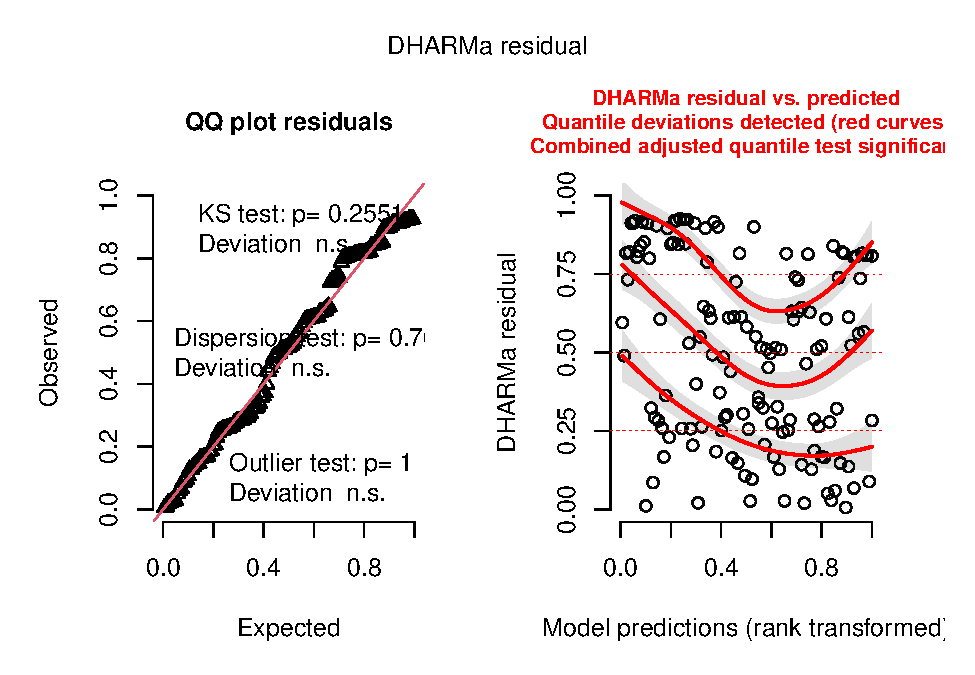
\includegraphics[keepaspectratio]{ch1_glm_clean_files/figure-latex/unnamed-chunk-3-1.pdf}}

\begin{enumerate}
\def\labelenumi{\arabic{enumi})}
\setcounter{enumi}{2}
\tightlist
\item
  Try negative binomial instead and check diagnostics.
\end{enumerate}

\begin{itemize}
\tightlist
\item
  Combined adjusted quantile test still significant.
\end{itemize}

\begin{Shaded}
\begin{Highlighting}[]
\NormalTok{burrows\_siteOnly\_negBin }\OtherTok{\textless{}{-}} \FunctionTok{glmmTMB}\NormalTok{(num\_burrows }\SpecialCharTok{\textasciitilde{}}\NormalTok{ grass\_forb\_perc\_scaled }\SpecialCharTok{+} 
\NormalTok{                             (}\DecValTok{1}\SpecialCharTok{|}\NormalTok{site\_id),}
                           \AttributeTok{family =}\NormalTok{ nbinom2, }
                           \AttributeTok{data =}\NormalTok{ field\_data)}

\CommentTok{\#simulate residuals}
\NormalTok{residuals\_burrows\_siteOnly\_negBin }\OtherTok{\textless{}{-}} \FunctionTok{simulateResiduals}\NormalTok{(}\AttributeTok{fittedModel =}\NormalTok{ burrows\_siteOnly\_negBin, }\AttributeTok{plot =} \ConstantTok{TRUE}\NormalTok{)}
\end{Highlighting}
\end{Shaded}

\pandocbounded{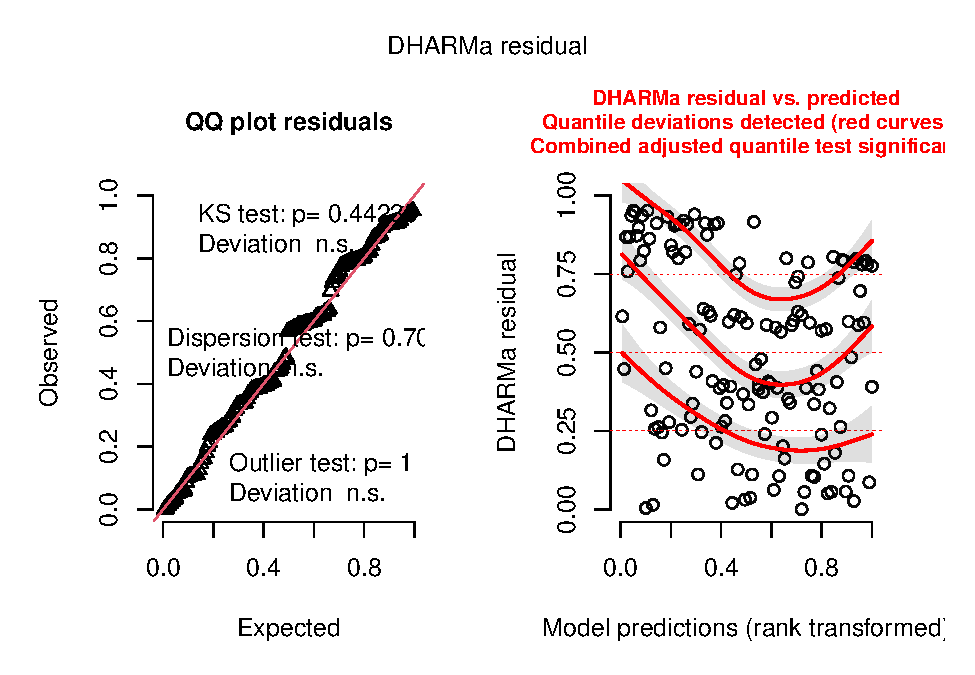
\includegraphics[keepaspectratio]{ch1_glm_clean_files/figure-latex/unnamed-chunk-4-1.pdf}}

\begin{enumerate}
\def\labelenumi{\arabic{enumi})}
\setcounter{enumi}{3}
\tightlist
\item
  Try zero-inflated poisson and check diagnostics.
\end{enumerate}

\begin{itemize}
\tightlist
\item
  combined adjusted quantile test still significant.
\end{itemize}

\begin{Shaded}
\begin{Highlighting}[]
\NormalTok{burrows\_zi\_pois }\OtherTok{\textless{}{-}} \FunctionTok{glmmTMB}\NormalTok{(num\_burrows }\SpecialCharTok{\textasciitilde{}}\NormalTok{ grass\_forb\_perc\_scaled }\SpecialCharTok{+} 
\NormalTok{                             (}\DecValTok{1}\SpecialCharTok{|}\NormalTok{site\_id),}
                           \AttributeTok{ziformula =} \SpecialCharTok{\textasciitilde{}}\NormalTok{ grass\_forb\_perc\_scaled }\SpecialCharTok{+} 
\NormalTok{                             (}\DecValTok{1}\SpecialCharTok{|}\NormalTok{site\_id),}
                           \AttributeTok{family =}\NormalTok{ poisson, }
                           \AttributeTok{data =}\NormalTok{ field\_data)}

\CommentTok{\#simulate residuals}
\NormalTok{residuals\_burrows\_zi }\OtherTok{\textless{}{-}} \FunctionTok{simulateResiduals}\NormalTok{(}\AttributeTok{fittedModel =}\NormalTok{ burrows\_zi\_pois, }\AttributeTok{plot =} \ConstantTok{TRUE}\NormalTok{)}
\end{Highlighting}
\end{Shaded}

\pandocbounded{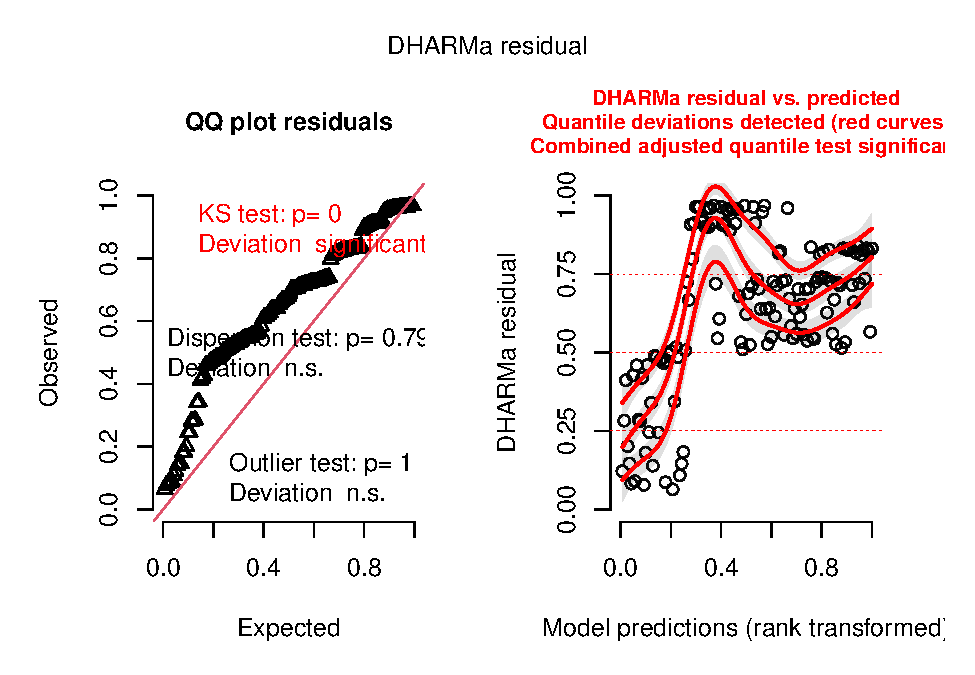
\includegraphics[keepaspectratio]{ch1_glm_clean_files/figure-latex/unnamed-chunk-5-1.pdf}}

\begin{enumerate}
\def\labelenumi{\arabic{enumi})}
\setcounter{enumi}{4}
\tightlist
\item
  Try zero-inflated negative binomial and check diagnostics.
\end{enumerate}

\begin{itemize}
\tightlist
\item
  combined adjusted quantile test still significant.
\end{itemize}

\begin{Shaded}
\begin{Highlighting}[]
\NormalTok{burrows\_zi\_nbin }\OtherTok{\textless{}{-}} \FunctionTok{glmmTMB}\NormalTok{(num\_burrows }\SpecialCharTok{\textasciitilde{}}\NormalTok{ grass\_forb\_perc\_scaled }\SpecialCharTok{+} 
\NormalTok{                             (}\DecValTok{1}\SpecialCharTok{|}\NormalTok{site\_id),}
                           \AttributeTok{ziformula =} \SpecialCharTok{\textasciitilde{}}\NormalTok{ grass\_forb\_perc\_scaled }\SpecialCharTok{+} 
\NormalTok{                             (}\DecValTok{1}\SpecialCharTok{|}\NormalTok{site\_id),}
                           \AttributeTok{family =}\NormalTok{ nbinom2, }
                           \AttributeTok{data =}\NormalTok{ field\_data)}

\CommentTok{\#simulate residuals}
\NormalTok{residuals\_burrows\_zi\_nbin }\OtherTok{\textless{}{-}} \FunctionTok{simulateResiduals}\NormalTok{(}\AttributeTok{fittedModel =}\NormalTok{ burrows\_zi\_nbin, }\AttributeTok{plot =} \ConstantTok{TRUE}\NormalTok{)}
\end{Highlighting}
\end{Shaded}

\begin{verbatim}
## Warning in newton(lsp = lsp, X = G$X, y = G$y, Eb = G$Eb, UrS = G$UrS, L = G$L,
## : Fitting terminated with step failure - check results carefully
\end{verbatim}

\pandocbounded{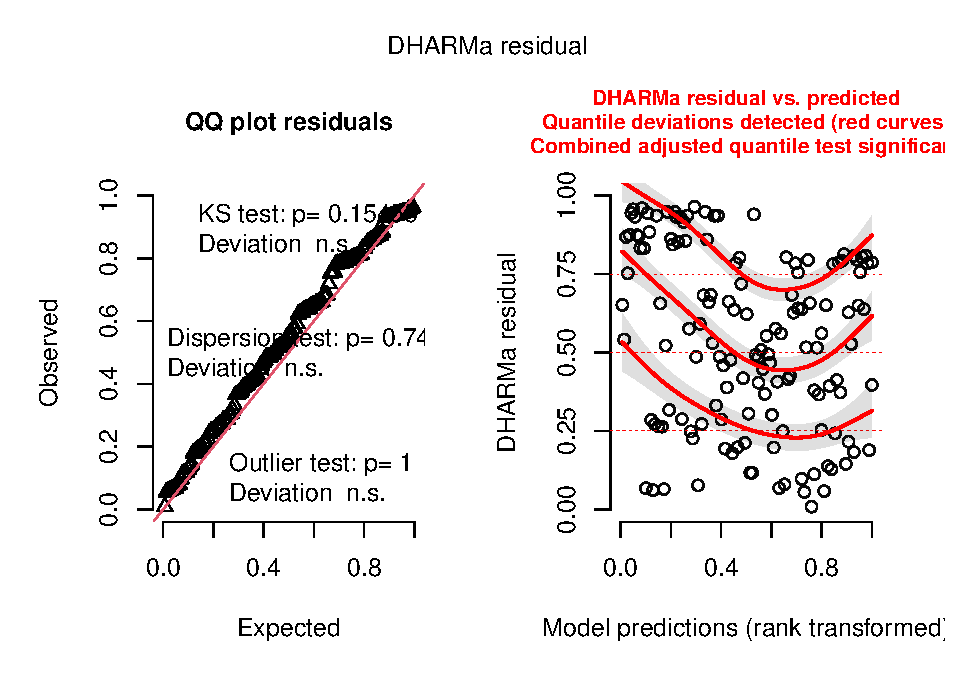
\includegraphics[keepaspectratio]{ch1_glm_clean_files/figure-latex/unnamed-chunk-6-1.pdf}}

\begin{Shaded}
\begin{Highlighting}[]
\CommentTok{\#signficant KS test and combined adjusted quantile test}
\end{Highlighting}
\end{Shaded}

\begin{enumerate}
\def\labelenumi{\arabic{enumi})}
\setcounter{enumi}{5}
\tightlist
\item
  Stick with poisson but try using categorical cover\_type as predictor
  instead of \% grass/forb cover and try different random effect
  structures.
\end{enumerate}

\begin{itemize}
\tightlist
\item
  models using continuous percent grass/forb cover as a predictor showed
  poor fit and significant residual patterns, likely due to the small
  sample size (n = 24). Because sites were grouped into two distinct
  habitat types---grassy plots with high vegetation cover and bare plots
  with little or no cover---the variable was reclassified as a
  categorical factor (``grass'' vs.~``bare''). This simplified model
  structure improved residual diagnostics and provided a clearer
  ecological interpretation of differences in burrow abundance between
  habitat types.
\end{itemize}

\begin{Shaded}
\begin{Highlighting}[]
\NormalTok{burrows\_cover\_full }\OtherTok{\textless{}{-}} \FunctionTok{glmmTMB}\NormalTok{(num\_burrows }\SpecialCharTok{\textasciitilde{}}\NormalTok{ cover\_type }\SpecialCharTok{+} 
\NormalTok{                             (}\DecValTok{1}\SpecialCharTok{|}\NormalTok{area}\SpecialCharTok{/}\NormalTok{site\_id),}
                           \AttributeTok{family =}\NormalTok{ poisson, }
                           \AttributeTok{data =}\NormalTok{ field\_data)}

\NormalTok{burrows\_cover\_siteOnly }\OtherTok{\textless{}{-}} \FunctionTok{glmmTMB}\NormalTok{(num\_burrows }\SpecialCharTok{\textasciitilde{}}\NormalTok{ cover\_type }\SpecialCharTok{+} 
\NormalTok{                             (}\DecValTok{1}\SpecialCharTok{|}\NormalTok{site\_id),}
                           \AttributeTok{family =}\NormalTok{ poisson, }
                           \AttributeTok{data =}\NormalTok{ field\_data)}

\NormalTok{burrows\_cover\_areaOnly }\OtherTok{\textless{}{-}} \FunctionTok{glmmTMB}\NormalTok{(num\_burrows }\SpecialCharTok{\textasciitilde{}}\NormalTok{ cover\_type }\SpecialCharTok{+} 
\NormalTok{                             (}\DecValTok{1}\SpecialCharTok{|}\NormalTok{area),}
                           \AttributeTok{family =}\NormalTok{ poisson, }
                           \AttributeTok{data =}\NormalTok{ field\_data)}


\CommentTok{\#compare models using maximum likelihood test}
\FunctionTok{anova}\NormalTok{(burrows\_cover\_full, burrows\_cover\_siteOnly, burrows\_cover\_areaOnly)}
\end{Highlighting}
\end{Shaded}

\begin{verbatim}
## Data: field_data
## Models:
## burrows_cover_siteOnly: num_burrows ~ cover_type + (1 | site_id), zi=~0, disp=~1
## burrows_cover_areaOnly: num_burrows ~ cover_type + (1 | area), zi=~0, disp=~1
## burrows_cover_full: num_burrows ~ cover_type + (1 | area/site_id), zi=~0, disp=~1
##                        Df    AIC    BIC   logLik deviance  Chisq Chi Df
## burrows_cover_siteOnly  3 1668.2 1677.0  -831.11   1662.2              
## burrows_cover_areaOnly  3 2664.6 2673.4 -1329.28   2658.6   0.00      0
## burrows_cover_full      4 1667.7 1679.5  -829.87   1659.7 998.81      1
##                        Pr(>Chisq)    
## burrows_cover_siteOnly               
## burrows_cover_areaOnly          1    
## burrows_cover_full         <2e-16 ***
## ---
## Signif. codes:  0 '***' 0.001 '**' 0.01 '*' 0.05 '.' 0.1 ' ' 1
\end{verbatim}

\begin{Shaded}
\begin{Highlighting}[]
\DocumentationTok{\#\#full model is best (lowest AIC)}
\end{Highlighting}
\end{Shaded}

\begin{enumerate}
\def\labelenumi{\arabic{enumi}.}
\setcounter{enumi}{6}
\tightlist
\item
  Check diagnostics
\end{enumerate}

\begin{itemize}
\tightlist
\item
  significant within-group deviations from uniformity
\end{itemize}

\begin{Shaded}
\begin{Highlighting}[]
\CommentTok{\#simulate residuals}
\NormalTok{residuals\_burrows\_cover\_full }\OtherTok{\textless{}{-}} \FunctionTok{simulateResiduals}\NormalTok{(}\AttributeTok{fittedModel =}\NormalTok{ burrows\_cover\_full, }\AttributeTok{plot =} \ConstantTok{TRUE}\NormalTok{)}
\end{Highlighting}
\end{Shaded}

\pandocbounded{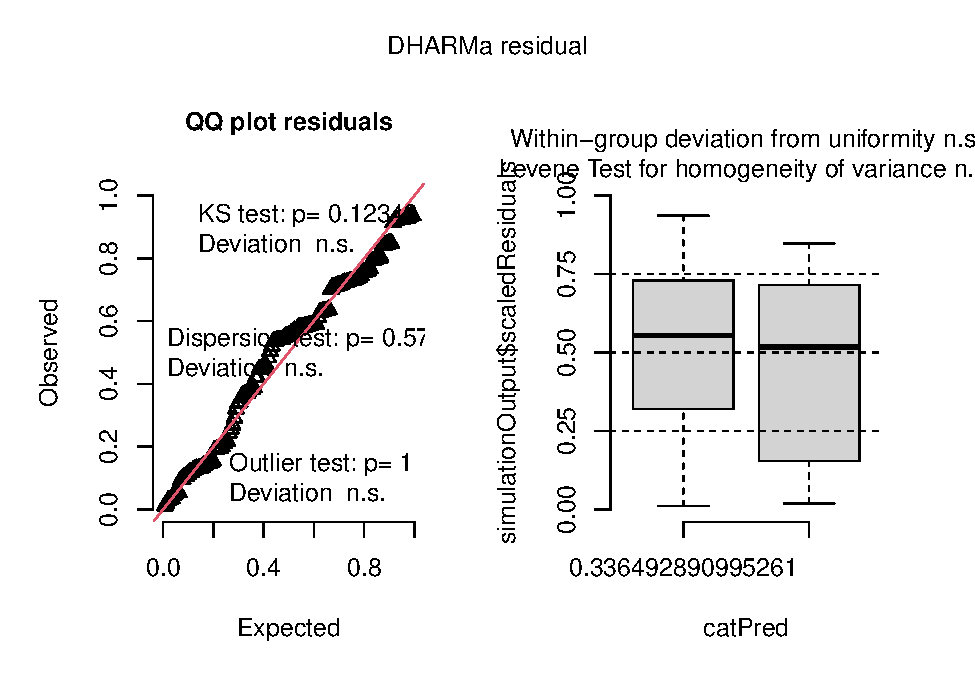
\includegraphics[keepaspectratio]{ch1_glm_clean_files/figure-latex/unnamed-chunk-8-1.pdf}}

\begin{enumerate}
\def\labelenumi{\arabic{enumi}.}
\setcounter{enumi}{7}
\tightlist
\item
  Try simpler random effect structure (site-only) and re-check
  diagnostics
\end{enumerate}

\begin{itemize}
\tightlist
\item
  No significant problems detected.
\end{itemize}

\begin{Shaded}
\begin{Highlighting}[]
\CommentTok{\#simulate residuals}
\NormalTok{residuals\_burrows\_cover\_siteOnly }\OtherTok{\textless{}{-}} \FunctionTok{simulateResiduals}\NormalTok{(}\AttributeTok{fittedModel =}\NormalTok{ burrows\_cover\_siteOnly, }\AttributeTok{plot =} \ConstantTok{TRUE}\NormalTok{)}
\end{Highlighting}
\end{Shaded}

\pandocbounded{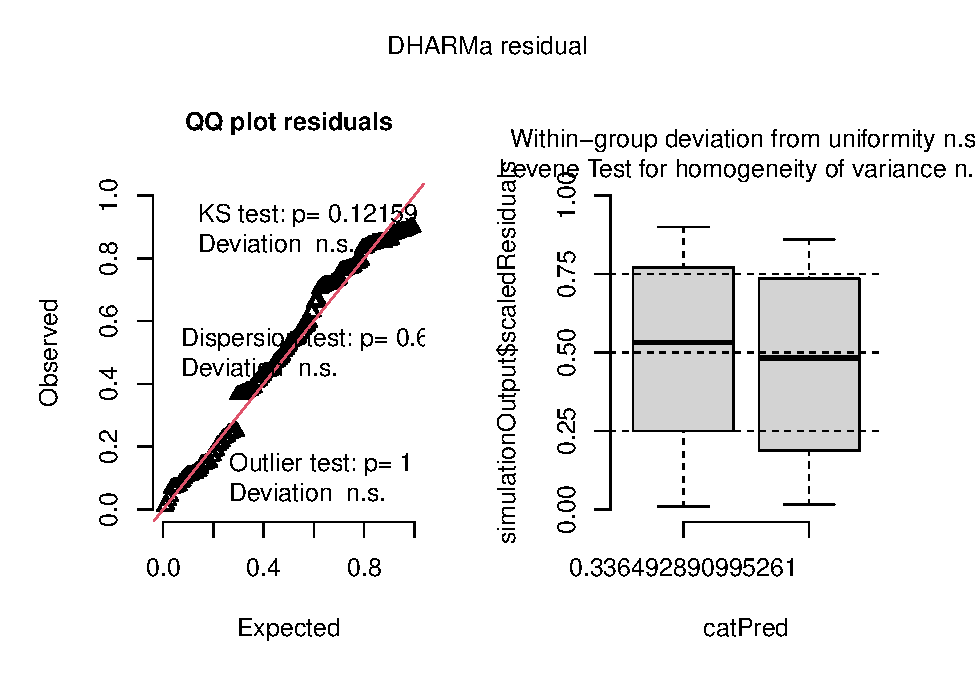
\includegraphics[keepaspectratio]{ch1_glm_clean_files/figure-latex/unnamed-chunk-9-1.pdf}}

\begin{enumerate}
\def\labelenumi{\arabic{enumi}.}
\setcounter{enumi}{8}
\tightlist
\item
  Plot results
\end{enumerate}

\begin{Shaded}
\begin{Highlighting}[]
\FunctionTok{summary}\NormalTok{(burrows\_cover\_siteOnly)}
\end{Highlighting}
\end{Shaded}

\begin{verbatim}
##  Family: poisson  ( log )
## Formula:          num_burrows ~ cover_type + (1 | site_id)
## Data: field_data
## 
##       AIC       BIC    logLik -2*log(L)  df.resid 
##    1668.2    1677.0    -831.1    1662.2       137 
## 
## Random effects:
## 
## Conditional model:
##  Groups  Name        Variance Std.Dev.
##  site_id (Intercept) 3.825    1.956   
## Number of obs: 140, groups:  site_id, 12
## 
## Conditional model:
##                 Estimate Std. Error z value Pr(>|z|)  
## (Intercept)       0.6365     0.8271   0.770   0.4415  
## cover_typegrass   1.9894     1.1510   1.728   0.0839 .
## ---
## Signif. codes:  0 '***' 0.001 '**' 0.01 '*' 0.05 '.' 0.1 ' ' 1
\end{verbatim}

\subsection{Plots}\label{plots}

Number of rodent burrows vs cover type

\begin{Shaded}
\begin{Highlighting}[]
\CommentTok{\#create new data grid}
\NormalTok{rodent\_data\_cover}\OtherTok{\textless{}{-}} \FunctionTok{expand.grid}\NormalTok{(}
  \AttributeTok{cover\_type =} \FunctionTok{unique}\NormalTok{(field\_data}\SpecialCharTok{$}\NormalTok{cover\_type)}
\NormalTok{)}

\CommentTok{\# Get predicted probabilities and standard errors}
\NormalTok{pred\_rodent\_cover }\OtherTok{\textless{}{-}} \FunctionTok{predict}\NormalTok{(burrows\_cover\_siteOnly,}
                            \AttributeTok{newdata =}\NormalTok{ rodent\_data\_cover,}
                            \AttributeTok{type =} \StringTok{"link"}\NormalTok{,}
                            \AttributeTok{se.fit =} \ConstantTok{TRUE}\NormalTok{,}
                            \AttributeTok{re.form =} \ConstantTok{NA}\NormalTok{)}

\CommentTok{\# Combine predictions with data frame}
\NormalTok{pred\_rodent\_cover\_df }\OtherTok{\textless{}{-}} \FunctionTok{cbind}\NormalTok{(rodent\_data\_cover,}
                 \AttributeTok{fit\_log =}\NormalTok{ pred\_rodent\_cover}\SpecialCharTok{$}\NormalTok{fit,}
                 \AttributeTok{se\_log =}\NormalTok{ pred\_rodent\_cover}\SpecialCharTok{$}\NormalTok{se.fit)}

\CommentTok{\#calculate predictions and confidence intervals on response scale (not log scale)}
\NormalTok{pred\_rodent\_cover\_df }\OtherTok{\textless{}{-}}\NormalTok{ pred\_rodent\_cover\_df }\SpecialCharTok{\%\textgreater{}\%}
  \FunctionTok{mutate}\NormalTok{(}
    \AttributeTok{fit =} \FunctionTok{exp}\NormalTok{(fit\_log),}
    \AttributeTok{lower =} \FunctionTok{exp}\NormalTok{(fit\_log }\SpecialCharTok{{-}} \FloatTok{1.96} \SpecialCharTok{*}\NormalTok{ se\_log),}
    \AttributeTok{upper =} \FunctionTok{exp}\NormalTok{(fit\_log }\SpecialCharTok{+} \FloatTok{1.96} \SpecialCharTok{*}\NormalTok{ se\_log)}
\NormalTok{  )}


\FunctionTok{ggplot}\NormalTok{(pred\_rodent\_cover\_df, }\FunctionTok{aes}\NormalTok{(}\AttributeTok{x =}\NormalTok{ cover\_type, }\AttributeTok{y =}\NormalTok{ fit)) }\SpecialCharTok{+}
  \FunctionTok{geom\_point}\NormalTok{(}\AttributeTok{size =} \DecValTok{8}\NormalTok{) }\SpecialCharTok{+}
  \FunctionTok{geom\_errorbar}\NormalTok{(}\FunctionTok{aes}\NormalTok{(}\AttributeTok{ymin =}\NormalTok{ lower, }\AttributeTok{ymax =}\NormalTok{ upper), }\AttributeTok{width =} \FloatTok{0.2}\NormalTok{, }\AttributeTok{position =} \FunctionTok{position\_dodge}\NormalTok{(}\FloatTok{0.6}\NormalTok{), }\AttributeTok{linewidth =} \FloatTok{1.5}\NormalTok{) }\SpecialCharTok{+}
  \FunctionTok{labs}\NormalTok{(}\AttributeTok{x =} \StringTok{"Cover type"}\NormalTok{,}
       \AttributeTok{y =} \StringTok{"Predicted burrow count}\SpecialCharTok{\textbackslash{}n}\StringTok{(per plot)"}\NormalTok{) }\SpecialCharTok{+}
  \FunctionTok{theme\_classic}\NormalTok{(}\AttributeTok{base\_size =} \DecValTok{23}\NormalTok{)}
\end{Highlighting}
\end{Shaded}

\pandocbounded{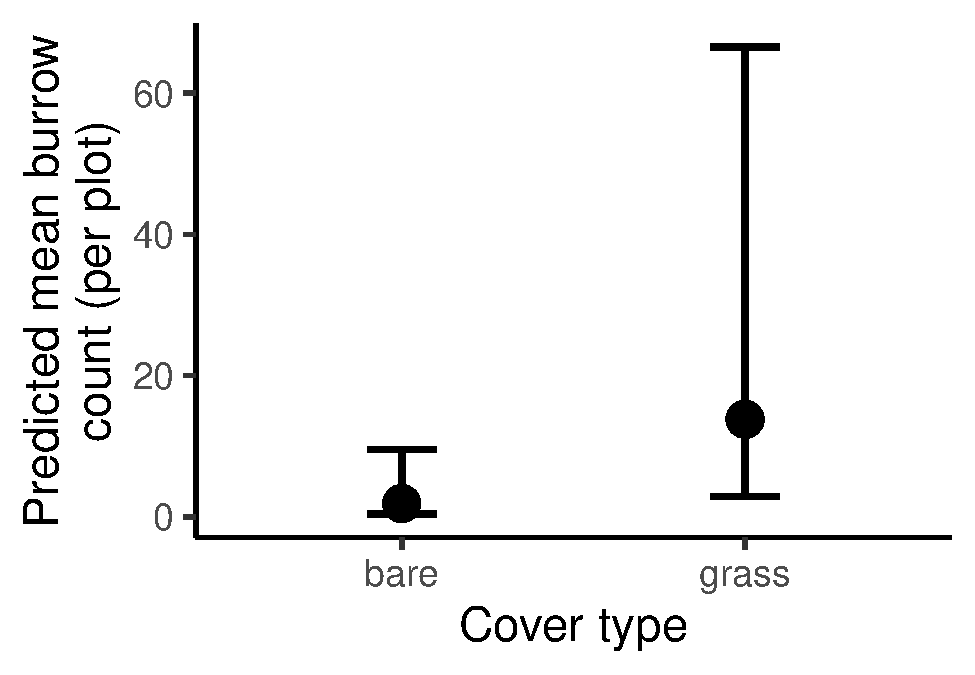
\includegraphics[keepaspectratio]{ch1_glm_clean_files/figure-latex/unnamed-chunk-11-1.pdf}}

\subsection{Findings}\label{findings}

Neither grass + forb \% nor julian date had significant effects on
rodent burrow abundance. However, cover type showed a marginally
insignificant trend (p=0.0839), where grassy sites had a higher
abundance of burrows.

\section{Rodent burrow vacancy
analysis}\label{rodent-burrow-vacancy-analysis}

I want to determine what influences the proportion of burrows that are
inactive (available as nest sites for bumble bees) across my sites.

\subsection{Steps}\label{steps-1}

\begin{enumerate}
\def\labelenumi{\arabic{enumi})}
\item
  Try different random effect structures in a binomial model. Compare
  alternative random effect structures using maximum likelihood (ML) via
  AIC. I did not include plot as a random effect structure since there
  was only one observation per plot for rodent burrow data.

\begin{Shaded}
\begin{Highlighting}[]
\NormalTok{burrows\_vacancy\_full }\OtherTok{\textless{}{-}} \FunctionTok{glmmTMB}\NormalTok{(}
  \FunctionTok{cbind}\NormalTok{(num\_inactive\_burrows, num\_active\_burrows) }\CommentTok{\#tells the model that successes = number of inactive (vacant) burrows and failures = number of active burrows}
  \SpecialCharTok{\textasciitilde{}}\NormalTok{ cover\_type }\SpecialCharTok{+}\NormalTok{ (}\DecValTok{1}\SpecialCharTok{|}\NormalTok{area}\SpecialCharTok{/}\NormalTok{site\_id),}
  \AttributeTok{family =} \FunctionTok{binomial}\NormalTok{(}\AttributeTok{link =} \StringTok{"logit"}\NormalTok{), }
  \AttributeTok{data =}\NormalTok{ field\_data)}

\NormalTok{burrows\_vacancy\_siteOnly }\OtherTok{\textless{}{-}} \FunctionTok{glmmTMB}\NormalTok{(}
  \FunctionTok{cbind}\NormalTok{(num\_inactive\_burrows, num\_active\_burrows) }\CommentTok{\#tells the model that successes = number of inactive (vacant) burrows and failures = number of active burrows}
  \SpecialCharTok{\textasciitilde{}}\NormalTok{ cover\_type }\SpecialCharTok{+}\NormalTok{ (}\DecValTok{1}\SpecialCharTok{|}\NormalTok{site\_id),}
  \AttributeTok{family =} \FunctionTok{binomial}\NormalTok{(}\AttributeTok{link =} \StringTok{"logit"}\NormalTok{), }
  \AttributeTok{data =}\NormalTok{ field\_data)}

\NormalTok{burrows\_vacancy\_areaOnly }\OtherTok{\textless{}{-}} \FunctionTok{glmmTMB}\NormalTok{(}
  \FunctionTok{cbind}\NormalTok{(num\_inactive\_burrows, num\_active\_burrows) }\CommentTok{\#tells the model that successes = number of inactive (vacant) burrows and failures = number of active burrows}
  \SpecialCharTok{\textasciitilde{}}\NormalTok{ cover\_type }\SpecialCharTok{+}\NormalTok{ (}\DecValTok{1}\SpecialCharTok{|}\NormalTok{area),}
  \AttributeTok{family =} \FunctionTok{binomial}\NormalTok{(}\AttributeTok{link =} \StringTok{"logit"}\NormalTok{), }
  \AttributeTok{data =}\NormalTok{ field\_data)}


\CommentTok{\#compare models using maximum likelihood test}
\FunctionTok{anova}\NormalTok{(burrows\_vacancy\_full, burrows\_vacancy\_siteOnly, burrows\_vacancy\_areaOnly)}
\end{Highlighting}
\end{Shaded}

\begin{verbatim}
## Data: field_data
## Models:
## burrows_vacancy_siteOnly: cbind(num_inactive_burrows, num_active_burrows) ~ cover_type + , zi=~0, disp=~1
## burrows_vacancy_siteOnly:     (1 | site_id), zi=~0, disp=~1
## burrows_vacancy_areaOnly: cbind(num_inactive_burrows, num_active_burrows) ~ cover_type + , zi=~0, disp=~1
## burrows_vacancy_areaOnly:     (1 | area), zi=~0, disp=~1
## burrows_vacancy_full: cbind(num_inactive_burrows, num_active_burrows) ~ cover_type + , zi=~0, disp=~1
## burrows_vacancy_full:     (1 | area/site_id), zi=~0, disp=~1
##                          Df    AIC    BIC  logLik deviance  Chisq Chi Df
## burrows_vacancy_siteOnly  3 463.22 472.04 -228.61   457.22              
## burrows_vacancy_areaOnly  3 497.71 506.54 -245.86   491.71  0.000      0
## burrows_vacancy_full      4 465.22 476.98 -228.61   457.22 34.495      1
##                          Pr(>Chisq)    
## burrows_vacancy_siteOnly               
## burrows_vacancy_areaOnly          1    
## burrows_vacancy_full      4.273e-09 ***
## ---
## Signif. codes:  0 '***' 0.001 '**' 0.01 '*' 0.05 '.' 0.1 ' ' 1
\end{verbatim}

\begin{Shaded}
\begin{Highlighting}[]
\DocumentationTok{\#\#results tells us the burrows\_siteOnly is best model (lowest AIC)}
\end{Highlighting}
\end{Shaded}
\item
  Check diagnostics
\end{enumerate}

\begin{itemize}
\tightlist
\item
  The diagnostic plot indicates a significant KS test. The significant
  KS test likely reflects low variability in vacancy probabilities
  across farms, with vacancy rates clustering near 0.5, rather than
  substantive lack of fit. No evidence of overdispersion, zero
  inflation, outliers, or group-level structure was detected.
\end{itemize}

\begin{Shaded}
\begin{Highlighting}[]
\CommentTok{\#simulate residuals }
\NormalTok{residuals\_burrows\_vacancy\_siteOnly }\OtherTok{\textless{}{-}} \FunctionTok{simulateResiduals}\NormalTok{(}\AttributeTok{fittedModel =}\NormalTok{ burrows\_vacancy\_siteOnly, }\AttributeTok{plot =} \ConstantTok{TRUE}\NormalTok{)}
\end{Highlighting}
\end{Shaded}

\pandocbounded{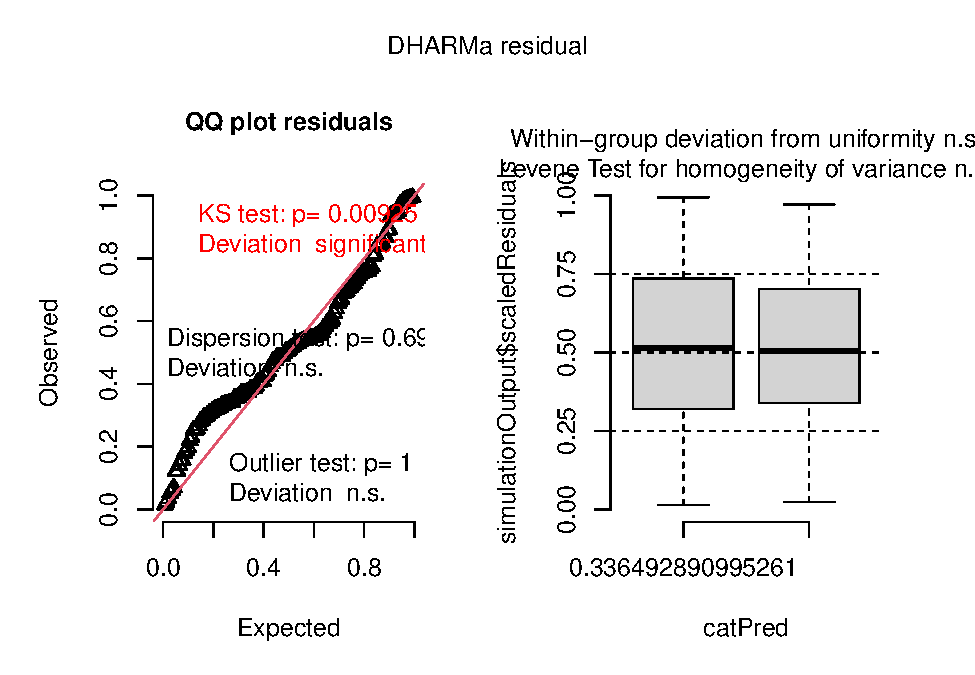
\includegraphics[keepaspectratio]{ch1_glm_clean_files/figure-latex/unnamed-chunk-13-1.pdf}}

\begin{Shaded}
\begin{Highlighting}[]
\DocumentationTok{\#\#KS test significant}
\end{Highlighting}
\end{Shaded}

\begin{enumerate}
\def\labelenumi{\arabic{enumi}.}
\setcounter{enumi}{2}
\tightlist
\item
  Print results
\end{enumerate}

\begin{Shaded}
\begin{Highlighting}[]
\FunctionTok{summary}\NormalTok{(burrows\_vacancy\_siteOnly)}
\end{Highlighting}
\end{Shaded}

\begin{verbatim}
##  Family: binomial  ( logit )
## Formula:          
## cbind(num_inactive_burrows, num_active_burrows) ~ cover_type +  
##     (1 | site_id)
## Data: field_data
## 
##       AIC       BIC    logLik -2*log(L)  df.resid 
##     463.2     472.0    -228.6     457.2       137 
## 
## Random effects:
## 
## Conditional model:
##  Groups  Name        Variance Std.Dev.
##  site_id (Intercept) 1.587    1.26    
## Number of obs: 140, groups:  site_id, 12
## 
## Conditional model:
##                  Estimate Std. Error z value Pr(>|z|)
## (Intercept)      0.006844   0.620445   0.011    0.991
## cover_typegrass -0.358816   0.831890  -0.431    0.666
\end{verbatim}

\subsection{Plots}\label{plots-1}

Proportion of vacant burrows vs cover type

\begin{Shaded}
\begin{Highlighting}[]
\CommentTok{\#create new data grid}
\NormalTok{vacancy\_data\_cover}\OtherTok{\textless{}{-}} \FunctionTok{expand.grid}\NormalTok{(}
  \AttributeTok{cover\_type =} \FunctionTok{unique}\NormalTok{(field\_data}\SpecialCharTok{$}\NormalTok{cover\_type)}
\NormalTok{)}

\CommentTok{\# Get predicted probabilities and standard errors}
\NormalTok{pred\_vacancy\_cover }\OtherTok{\textless{}{-}} \FunctionTok{predict}\NormalTok{(burrows\_vacancy\_siteOnly,}
                            \AttributeTok{newdata =}\NormalTok{ vacancy\_data\_cover,}
                            \AttributeTok{type =} \StringTok{"link"}\NormalTok{,}
                            \AttributeTok{se.fit =} \ConstantTok{TRUE}\NormalTok{,}
                            \AttributeTok{re.form =} \ConstantTok{NA}\NormalTok{)}

\CommentTok{\# Combine predictions with data frame}
\NormalTok{pred\_vacancy\_cover\_df }\OtherTok{\textless{}{-}} \FunctionTok{cbind}\NormalTok{(vacancy\_data\_cover,}
                 \AttributeTok{fit\_logit =}\NormalTok{ pred\_vacancy\_cover}\SpecialCharTok{$}\NormalTok{fit,}
                 \AttributeTok{se\_logit =}\NormalTok{ pred\_vacancy\_cover}\SpecialCharTok{$}\NormalTok{se.fit)}

\CommentTok{\#calculate predictions and confidence intervals on response scale (not logit scale)}
\NormalTok{pred\_vacancy\_cover\_df }\OtherTok{\textless{}{-}}\NormalTok{ pred\_vacancy\_cover\_df }\SpecialCharTok{\%\textgreater{}\%}
  \FunctionTok{mutate}\NormalTok{(}
    \AttributeTok{fit =} \FunctionTok{plogis}\NormalTok{(fit\_logit),}
    \AttributeTok{lower =} \FunctionTok{plogis}\NormalTok{(fit\_logit }\SpecialCharTok{{-}} \FloatTok{1.96} \SpecialCharTok{*}\NormalTok{ se\_logit),}
    \AttributeTok{upper =} \FunctionTok{plogis}\NormalTok{(fit\_logit }\SpecialCharTok{+} \FloatTok{1.96} \SpecialCharTok{*}\NormalTok{ se\_logit)}
\NormalTok{  )}


\FunctionTok{ggplot}\NormalTok{(pred\_vacancy\_cover\_df, }\FunctionTok{aes}\NormalTok{(}\AttributeTok{x =}\NormalTok{ cover\_type, }\AttributeTok{y =}\NormalTok{ fit)) }\SpecialCharTok{+}
  \FunctionTok{geom\_point}\NormalTok{(}\AttributeTok{size =} \DecValTok{8}\NormalTok{) }\SpecialCharTok{+}
  \FunctionTok{geom\_errorbar}\NormalTok{(}\FunctionTok{aes}\NormalTok{(}\AttributeTok{ymin =}\NormalTok{ lower, }\AttributeTok{ymax =}\NormalTok{ upper), }\AttributeTok{width =} \FloatTok{0.2}\NormalTok{, }\AttributeTok{position =} \FunctionTok{position\_dodge}\NormalTok{(}\FloatTok{0.6}\NormalTok{), }\AttributeTok{linewidth =} \FloatTok{1.5}\NormalTok{) }\SpecialCharTok{+}
  \FunctionTok{labs}\NormalTok{(}\AttributeTok{x =} \StringTok{"Cover type"}\NormalTok{,}
       \AttributeTok{y =} \StringTok{"Predicted proportion}\SpecialCharTok{\textbackslash{}n}\StringTok{of vacant burrows}\SpecialCharTok{\textbackslash{}n}\StringTok{(per plot)"}\NormalTok{) }\SpecialCharTok{+}
  \FunctionTok{theme\_classic}\NormalTok{(}\AttributeTok{base\_size =} \DecValTok{23}\NormalTok{)}
\end{Highlighting}
\end{Shaded}

\pandocbounded{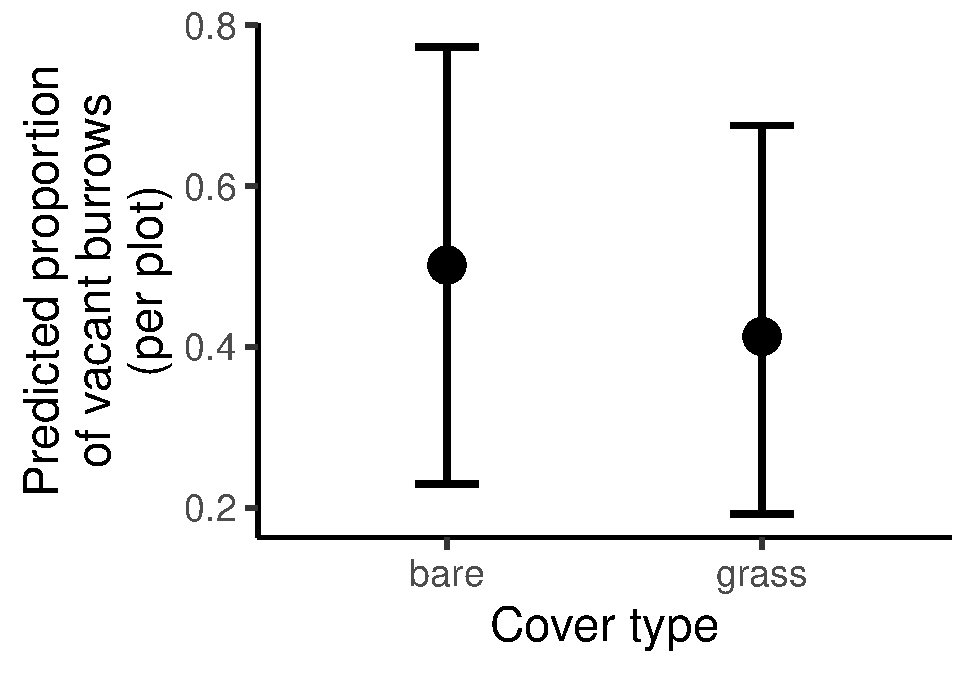
\includegraphics[keepaspectratio]{ch1_glm_clean_files/figure-latex/unnamed-chunk-15-1.pdf}}

\subsection{Findings}\label{findings-1}

There was not a significant difference in burrow vacancy probability
between grassy and bare sites (log-odds difference = --0.36, SE = 0.83,
\emph{p} = 0.67). Burrow vacancy probability was approximately 50\%
across sites, meaning that roughly one in two burrows at blueberry farms
in this study were available as potential nest sites for bumble bees.

\section{Floral abundance vs field management
(\%grass+forb)}\label{floral-abundance-vs-field-management-grassforb}

Use cumulative link model aka ordinal logistic regression because
bombus-relevant floral abundance has:

\begin{itemize}
\item
  discrete levels (0-5 scale) representing binned counts of blooms
\item
  ordered categories (higher numbers represent more blooms)
\item
  unequal intervals between categories
\end{itemize}

\subsection{Steps}\label{steps-2}

\begin{enumerate}
\def\labelenumi{\arabic{enumi})}
\tightlist
\item
  Tried running CLM with different random effect structures (full =
  1\textbar area/site/plot) then compared AIC values to determine best
  model.
\end{enumerate}

\begin{itemize}
\tightlist
\item
  determined that model without random effect had best fit
\end{itemize}

\begin{Shaded}
\begin{Highlighting}[]
\NormalTok{floral\_full }\OtherTok{\textless{}{-}} \FunctionTok{clmm}\NormalTok{(}\FunctionTok{as.factor}\NormalTok{(bombus\_floral\_abun) }\SpecialCharTok{\textasciitilde{}}\NormalTok{ cover\_type }\SpecialCharTok{+}
\NormalTok{                         julian.date\_scaled }\SpecialCharTok{+} 
\NormalTok{                         (}\DecValTok{1}\SpecialCharTok{|}\NormalTok{area}\SpecialCharTok{/}\NormalTok{site\_id}\SpecialCharTok{/}\NormalTok{plot\_id),}
                       \AttributeTok{link =} \StringTok{"logit"}\NormalTok{, }
                       \AttributeTok{data =}\NormalTok{ field\_data)}

\NormalTok{floral\_noArea }\OtherTok{\textless{}{-}} \FunctionTok{clmm}\NormalTok{(}\FunctionTok{as.factor}\NormalTok{(bombus\_floral\_abun) }\SpecialCharTok{\textasciitilde{}}\NormalTok{ cover\_type }\SpecialCharTok{+}
\NormalTok{                         julian.date\_scaled }\SpecialCharTok{+} 
\NormalTok{                         (}\DecValTok{1}\SpecialCharTok{|}\NormalTok{site\_id}\SpecialCharTok{/}\NormalTok{plot\_id),}
                       \AttributeTok{link =} \StringTok{"logit"}\NormalTok{, }
                       \AttributeTok{data =}\NormalTok{ field\_data)}

\CommentTok{\#floral\_plotOnly \textless{}{-} clmm(as.factor(bombus\_floral\_abun) \textasciitilde{} cover\_type +}
 \CommentTok{\#                        julian.date\_scaled + }
  \CommentTok{\#                       (1|plot\_id),}
   \CommentTok{\#                    link = "logit", }
    \CommentTok{\#                   data = field\_data)}
\DocumentationTok{\#\#can\textquotesingle{}t use since there are only 2 levels}

\NormalTok{floral\_siteOnly }\OtherTok{\textless{}{-}} \FunctionTok{clmm}\NormalTok{(}\FunctionTok{as.factor}\NormalTok{(bombus\_floral\_abun) }\SpecialCharTok{\textasciitilde{}}\NormalTok{ cover\_type }\SpecialCharTok{+}
\NormalTok{                         julian.date\_scaled }\SpecialCharTok{+} 
\NormalTok{                         (}\DecValTok{1}\SpecialCharTok{|}\NormalTok{site\_id),}
                       \AttributeTok{link =} \StringTok{"logit"}\NormalTok{, }
                       \AttributeTok{data =}\NormalTok{ field\_data)}

\NormalTok{floral\_AreaPlot }\OtherTok{\textless{}{-}} \FunctionTok{clmm}\NormalTok{(}\FunctionTok{as.factor}\NormalTok{(bombus\_floral\_abun) }\SpecialCharTok{\textasciitilde{}}\NormalTok{ cover\_type }\SpecialCharTok{+}
\NormalTok{                         julian.date\_scaled }\SpecialCharTok{+} 
\NormalTok{                         (}\DecValTok{1}\SpecialCharTok{|}\NormalTok{area}\SpecialCharTok{/}\NormalTok{plot\_id),}
                       \AttributeTok{link =} \StringTok{"logit"}\NormalTok{, }
                       \AttributeTok{data =}\NormalTok{ field\_data)}
\NormalTok{floral\_noRE }\OtherTok{\textless{}{-}} \FunctionTok{polr}\NormalTok{(}\FunctionTok{as.factor}\NormalTok{(bombus\_floral\_abun) }\SpecialCharTok{\textasciitilde{}}\NormalTok{ cover\_type }\SpecialCharTok{+}
\NormalTok{                         julian.date\_scaled,}
                       \AttributeTok{method =} \StringTok{"logistic"}\NormalTok{, }
                       \AttributeTok{data =}\NormalTok{ field\_data)}

\CommentTok{\#compare models AIC}
\FunctionTok{AIC}\NormalTok{(floral\_full, floral\_noArea, floral\_siteOnly, floral\_AreaPlot, floral\_noRE)}
\end{Highlighting}
\end{Shaded}

\begin{verbatim}
##                 df      AIC
## floral_full      9 441.1731
## floral_noArea    8 439.1731
## floral_siteOnly  7 437.1731
## floral_AreaPlot  8 439.1731
## floral_noRE      6 435.1731
\end{verbatim}

\begin{Shaded}
\begin{Highlighting}[]
\DocumentationTok{\#\#shows that model without random effect has best fit}
\end{Highlighting}
\end{Shaded}

\begin{enumerate}
\def\labelenumi{\arabic{enumi}.}
\setcounter{enumi}{1}
\tightlist
\item
  Run final model and look at output
\end{enumerate}

\begin{Shaded}
\begin{Highlighting}[]
\FunctionTok{summary}\NormalTok{(floral\_noRE)}
\end{Highlighting}
\end{Shaded}

\begin{verbatim}
## 
## Re-fitting to get Hessian
\end{verbatim}

\begin{verbatim}
## Call:
## polr(formula = as.factor(bombus_floral_abun) ~ cover_type + julian.date_scaled, 
##     data = field_data, method = "logistic")
## 
## Coefficients:
##                       Value Std. Error  t value
## cover_typegrass     0.02647     0.3041  0.08702
## julian.date_scaled -0.23119     0.1527 -1.51417
## 
## Intercepts:
##     Value   Std. Error t value
## 0|1 -1.3986  0.2610    -5.3585
## 1|2 -0.9291  0.2414    -3.8493
## 2|3 -0.1853  0.2272    -0.8153
## 3|4  0.6192  0.2332     2.6559
## 
## Residual Deviance: 423.1731 
## AIC: 435.1731
\end{verbatim}

\subsection{Plots}\label{plots-2}

Vegetation

\begin{Shaded}
\begin{Highlighting}[]
\NormalTok{floral\_veg\_data }\OtherTok{\textless{}{-}} \FunctionTok{data.frame}\NormalTok{(}
  \AttributeTok{cover\_type =} \FunctionTok{factor}\NormalTok{(}\FunctionTok{c}\NormalTok{(}\StringTok{"bare"}\NormalTok{, }\StringTok{"grass"}\NormalTok{), }\AttributeTok{levels =} \FunctionTok{levels}\NormalTok{(field\_data}\SpecialCharTok{$}\NormalTok{cover\_type)),}
  \AttributeTok{julian.date\_scaled =} \FunctionTok{mean}\NormalTok{(field\_data}\SpecialCharTok{$}\NormalTok{julian.date\_scaled, }\AttributeTok{na.rm =} \ConstantTok{TRUE}\NormalTok{)}
\NormalTok{)}

\CommentTok{\# Get predicted response for cover\_type, holding other variables at their means }
\NormalTok{pred\_floral\_veg }\OtherTok{\textless{}{-}} \FunctionTok{predict}\NormalTok{(floral\_noRE,}
                      \AttributeTok{newdata =}\NormalTok{ floral\_veg\_data,}
                      \AttributeTok{type =} \StringTok{"prob"}\NormalTok{)}


\CommentTok{\# Convert to long dataframe for plotting}

\NormalTok{pred\_floral\_veg\_df }\OtherTok{\textless{}{-}} \FunctionTok{as.data.frame}\NormalTok{(pred\_floral\_veg) }\SpecialCharTok{\%\textgreater{}\%}
  \FunctionTok{mutate}\NormalTok{(}\AttributeTok{cover\_type =} \FunctionTok{rownames}\NormalTok{(pred\_floral\_veg)) }\SpecialCharTok{\%\textgreater{}\%}
  \FunctionTok{pivot\_longer}\NormalTok{(}\AttributeTok{cols =} \SpecialCharTok{{-}}\NormalTok{cover\_type, }\AttributeTok{names\_to =} \StringTok{"response"}\NormalTok{, }\AttributeTok{values\_to =} \StringTok{"prob"}\NormalTok{)}

\CommentTok{\# Convert cover\_type to factor with proper labels}
\NormalTok{pred\_floral\_veg\_df}\SpecialCharTok{$}\NormalTok{cover\_type }\OtherTok{\textless{}{-}} \FunctionTok{factor}\NormalTok{(pred\_floral\_veg\_df}\SpecialCharTok{$}\NormalTok{cover\_type,}
                                   \AttributeTok{levels =} \FunctionTok{c}\NormalTok{(}\DecValTok{1}\NormalTok{, }\DecValTok{2}\NormalTok{),}
                                   \AttributeTok{labels =} \FunctionTok{c}\NormalTok{(}\StringTok{"bare"}\NormalTok{, }\StringTok{"grass"}\NormalTok{))}

\FunctionTok{ggplot}\NormalTok{(pred\_floral\_veg\_df, }\FunctionTok{aes}\NormalTok{(}\AttributeTok{x =}\NormalTok{ cover\_type, }\AttributeTok{y =}\NormalTok{ prob, }\AttributeTok{fill =}\NormalTok{ response)) }\SpecialCharTok{+}
  \FunctionTok{geom\_bar}\NormalTok{(}\AttributeTok{stat =} \StringTok{"identity"}\NormalTok{, }\AttributeTok{position =} \FunctionTok{position\_dodge}\NormalTok{(}\AttributeTok{width =} \FloatTok{0.9}\NormalTok{), }\AttributeTok{width =} \FloatTok{0.8}\NormalTok{) }\SpecialCharTok{+}
  \FunctionTok{labs}\NormalTok{(}
    \AttributeTok{x =} \StringTok{"Cover type"}\NormalTok{,}
    \AttributeTok{y =} \StringTok{"Predicted probability"}\NormalTok{,}
    \AttributeTok{fill =} \StringTok{"Floral}\SpecialCharTok{\textbackslash{}n}\StringTok{abundance}\SpecialCharTok{\textbackslash{}n}\StringTok{category"}
\NormalTok{  ) }\SpecialCharTok{+}
  \FunctionTok{theme\_classic}\NormalTok{(}\AttributeTok{base\_size =} \DecValTok{23}\NormalTok{)}
\end{Highlighting}
\end{Shaded}

\pandocbounded{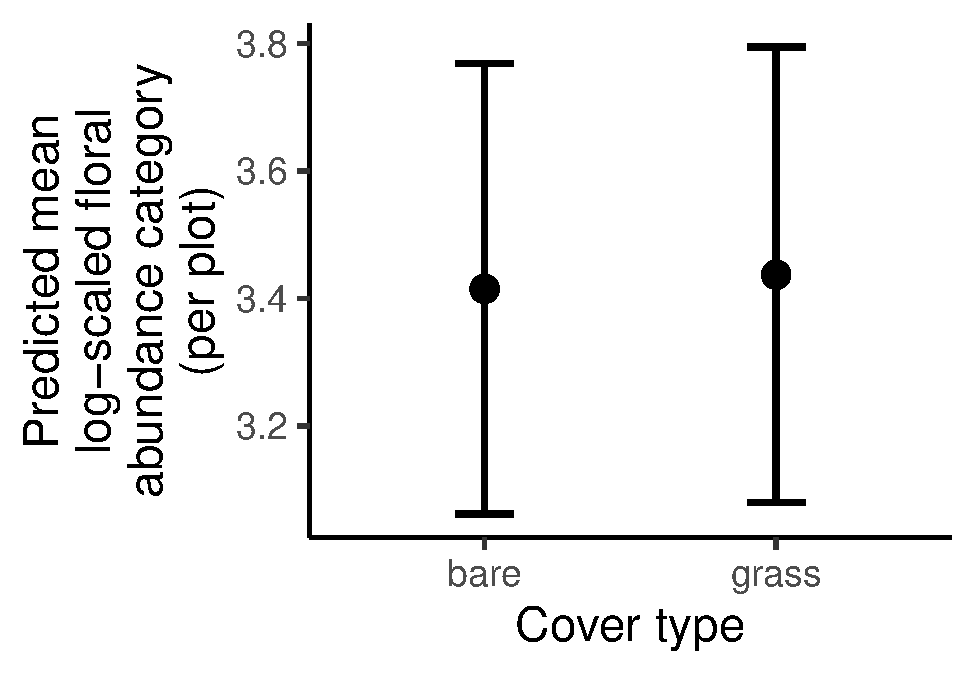
\includegraphics[keepaspectratio]{ch1_glm_clean_files/figure-latex/unnamed-chunk-18-1.pdf}}

Julian date

\begin{Shaded}
\begin{Highlighting}[]
\CommentTok{\# Define a sequence of values for grass\_forb\_perc\_scaled across its observed range}
\NormalTok{date\_seq }\OtherTok{\textless{}{-}} \FunctionTok{seq}\NormalTok{(}
  \AttributeTok{from =} \FunctionTok{min}\NormalTok{(field\_data}\SpecialCharTok{$}\NormalTok{julian.date\_scaled, }\AttributeTok{na.rm =} \ConstantTok{TRUE}\NormalTok{),}
  \AttributeTok{to =} \FunctionTok{max}\NormalTok{(field\_data}\SpecialCharTok{$}\NormalTok{julian.date\_scaled, }\AttributeTok{na.rm =} \ConstantTok{TRUE}\NormalTok{),}
  \AttributeTok{length.out =} \DecValTok{50}
\NormalTok{)}

\NormalTok{floral\_date\_data }\OtherTok{\textless{}{-}} \FunctionTok{data.frame}\NormalTok{(}
  \AttributeTok{cover\_type =} \StringTok{"grass"}\NormalTok{,}
  \AttributeTok{julian.date\_scaled =}\NormalTok{ date\_seq}
\NormalTok{)}

\CommentTok{\# Get predicted response for cover\_type, holding other variables at their means }
\NormalTok{pred\_floral\_date }\OtherTok{\textless{}{-}} \FunctionTok{predict}\NormalTok{(floral\_noRE,}
                      \AttributeTok{newdata =}\NormalTok{ floral\_date\_data,}
                      \AttributeTok{type =} \StringTok{"prob"}\NormalTok{)}


\CommentTok{\# Convert to long dataframe for plotting}
\NormalTok{pred\_floral\_date\_df }\OtherTok{\textless{}{-}} \FunctionTok{as.data.frame}\NormalTok{(pred\_floral\_date) }\SpecialCharTok{\%\textgreater{}\%}
  \FunctionTok{mutate}\NormalTok{(}\AttributeTok{julian.date\_scaled =}\NormalTok{ floral\_date\_data}\SpecialCharTok{$}\NormalTok{julian.date\_scaled) }\SpecialCharTok{\%\textgreater{}\%}
  \FunctionTok{pivot\_longer}\NormalTok{(}
    \AttributeTok{cols =} \DecValTok{0}\SpecialCharTok{:}\DecValTok{5}\NormalTok{,}
    \AttributeTok{names\_to =} \StringTok{"floral\_abun\_cat"}\NormalTok{,}
    \AttributeTok{values\_to =} \StringTok{"prob"}
\NormalTok{  )}

\FunctionTok{ggplot}\NormalTok{(pred\_floral\_date\_df, }\FunctionTok{aes}\NormalTok{(}\AttributeTok{x =}\NormalTok{ julian.date\_scaled, }\AttributeTok{y =}\NormalTok{ prob, }\AttributeTok{color =}\NormalTok{ floral\_abun\_cat)) }\SpecialCharTok{+}
  \FunctionTok{geom\_line}\NormalTok{(}\AttributeTok{linewidth =} \DecValTok{3}\NormalTok{) }\SpecialCharTok{+}
  \FunctionTok{labs}\NormalTok{(}
    \AttributeTok{x =} \StringTok{"Julian date (scaled)"}\NormalTok{,}
    \AttributeTok{y =} \StringTok{"Predicted probability"}\NormalTok{,}
    \AttributeTok{color =} \StringTok{"Floral}\SpecialCharTok{\textbackslash{}n}\StringTok{abundance}\SpecialCharTok{\textbackslash{}n}\StringTok{category"}
\NormalTok{  ) }\SpecialCharTok{+}
  \FunctionTok{theme\_classic}\NormalTok{(}\AttributeTok{base\_size =} \DecValTok{27}\NormalTok{)}
\end{Highlighting}
\end{Shaded}

\pandocbounded{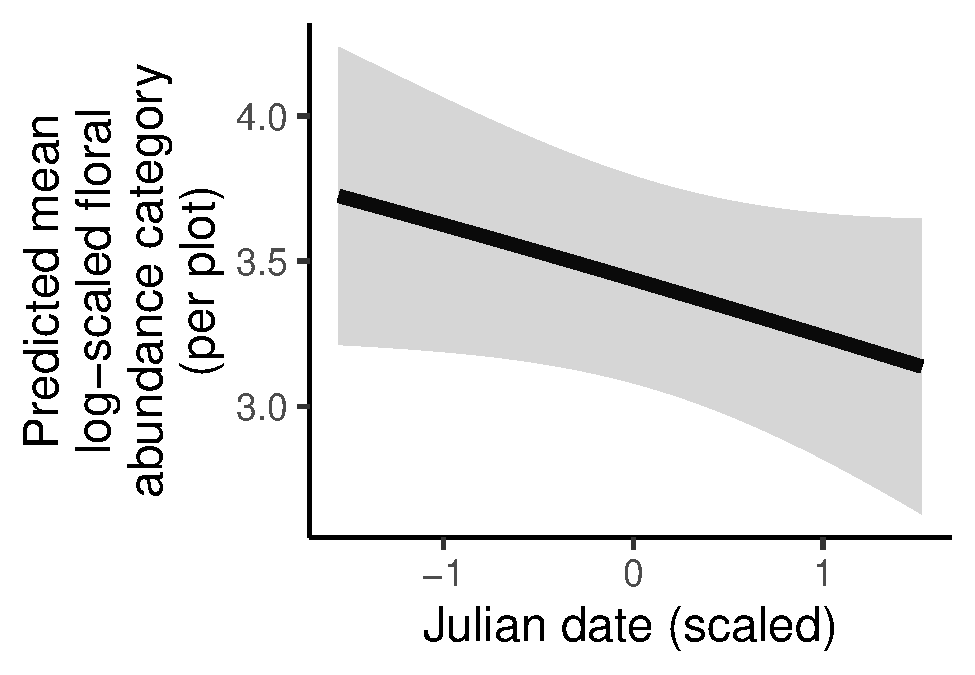
\includegraphics[keepaspectratio]{ch1_glm_clean_files/figure-latex/unnamed-chunk-19-1.pdf}}

\subsection{Findings}\label{findings-2}

No significant effect of either grass+ forb\% or julian date.

\section{Number of nest-searching queens vs flowers, rodents, and field
management
technique}\label{number-of-nest-searching-queens-vs-flowers-rodents-and-field-management-technique}

Start by plotting a zero-inflated poisson, since \# of nest-searching
queens is count data with a lot of zeros. I added bee\_season\_type as a
covariate, since during my exploratory data analyses I saw that there
was only a significant different in nest-searching queens among grassy
vs bare sites during nesting season.

\subsection{Steps}\label{steps-3}

\begin{enumerate}
\def\labelenumi{\arabic{enumi}.}
\tightlist
\item
  Try multiple random effects structures
\end{enumerate}

\begin{itemize}
\tightlist
\item
  best fit = no random effect
\end{itemize}

\begin{Shaded}
\begin{Highlighting}[]
\NormalTok{NSQ\_full }\OtherTok{\textless{}{-}} \FunctionTok{glmmTMB}\NormalTok{(nest\_searching\_queens }\SpecialCharTok{\textasciitilde{}}\NormalTok{ cover\_type }\SpecialCharTok{+} 
\NormalTok{                      bombus\_floral\_abun\_scaled }\SpecialCharTok{+} 
\NormalTok{                      num\_burrows\_scaled }\SpecialCharTok{+} 
\NormalTok{                      prop\_inactive\_scaled }\SpecialCharTok{+}
\NormalTok{                      bee\_season\_type }\SpecialCharTok{+} 
\NormalTok{                      (}\DecValTok{1}\SpecialCharTok{|}\NormalTok{area}\SpecialCharTok{/}\NormalTok{site\_id}\SpecialCharTok{/}\NormalTok{plot\_id),}
                    \AttributeTok{ziformula =} \SpecialCharTok{\textasciitilde{}}\NormalTok{ cover\_type }\SpecialCharTok{+} 
\NormalTok{                      bombus\_floral\_abun\_scaled }\SpecialCharTok{+} 
\NormalTok{                      num\_burrows\_scaled }\SpecialCharTok{+}
\NormalTok{                      prop\_inactive\_scaled }\SpecialCharTok{+}
\NormalTok{                      bee\_season\_type }\SpecialCharTok{+}
\NormalTok{                      (}\DecValTok{1}\SpecialCharTok{|}\NormalTok{area}\SpecialCharTok{/}\NormalTok{site\_id}\SpecialCharTok{/}\NormalTok{plot\_id),}
                    \AttributeTok{family =}\NormalTok{ poisson, }
                    \AttributeTok{data =}\NormalTok{ field\_data)}
\end{Highlighting}
\end{Shaded}

\begin{verbatim}
## Warning in finalizeTMB(TMBStruc, obj, fit, h, data.tmb.old): Model convergence
## problem; non-positive-definite Hessian matrix. See vignette('troubleshooting')
\end{verbatim}

\begin{Shaded}
\begin{Highlighting}[]
\NormalTok{NSQ\_noArea }\OtherTok{\textless{}{-}} \FunctionTok{glmmTMB}\NormalTok{(nest\_searching\_queens }\SpecialCharTok{\textasciitilde{}}\NormalTok{ cover\_type }\SpecialCharTok{+} 
\NormalTok{                        bombus\_floral\_abun\_scaled }\SpecialCharTok{+} 
\NormalTok{                        num\_burrows\_scaled }\SpecialCharTok{+} 
\NormalTok{                        prop\_inactive\_scaled }\SpecialCharTok{+}
\NormalTok{                        bee\_season\_type }\SpecialCharTok{+} 
\NormalTok{                        (}\DecValTok{1}\SpecialCharTok{|}\NormalTok{site\_id}\SpecialCharTok{/}\NormalTok{plot\_id),}
                      \AttributeTok{ziformula =} \SpecialCharTok{\textasciitilde{}}\NormalTok{ cover\_type }\SpecialCharTok{+} 
\NormalTok{                        bombus\_floral\_abun\_scaled }\SpecialCharTok{+} 
\NormalTok{                        num\_burrows\_scaled }\SpecialCharTok{+} 
\NormalTok{                        prop\_inactive\_scaled }\SpecialCharTok{+}
\NormalTok{                        bee\_season\_type }\SpecialCharTok{+}
\NormalTok{                        (}\DecValTok{1}\SpecialCharTok{|}\NormalTok{site\_id}\SpecialCharTok{/}\NormalTok{plot\_id),}
                      \AttributeTok{family =}\NormalTok{ poisson, }
                      \AttributeTok{data =}\NormalTok{ field\_data)}
\end{Highlighting}
\end{Shaded}

\begin{verbatim}
## Warning in finalizeTMB(TMBStruc, obj, fit, h, data.tmb.old): Model convergence
## problem; non-positive-definite Hessian matrix. See vignette('troubleshooting')
\end{verbatim}

\begin{Shaded}
\begin{Highlighting}[]
\NormalTok{NSQ\_plotOnly }\OtherTok{\textless{}{-}}  \FunctionTok{glmmTMB}\NormalTok{(nest\_searching\_queens }\SpecialCharTok{\textasciitilde{}}\NormalTok{ cover\_type }\SpecialCharTok{+} 
\NormalTok{                        bombus\_floral\_abun\_scaled }\SpecialCharTok{+} 
\NormalTok{                        num\_burrows\_scaled }\SpecialCharTok{+} 
\NormalTok{                        prop\_inactive\_scaled }\SpecialCharTok{+}
\NormalTok{                        bee\_season\_type }\SpecialCharTok{+} 
\NormalTok{                        (}\DecValTok{1}\SpecialCharTok{|}\NormalTok{plot\_id),}
                      \AttributeTok{ziformula =} \SpecialCharTok{\textasciitilde{}}\NormalTok{ cover\_type }\SpecialCharTok{+} 
\NormalTok{                        bombus\_floral\_abun\_scaled }\SpecialCharTok{+} 
\NormalTok{                        num\_burrows\_scaled }\SpecialCharTok{+} 
\NormalTok{                        prop\_inactive\_scaled }\SpecialCharTok{+}
\NormalTok{                        bee\_season\_type }\SpecialCharTok{+}
\NormalTok{                        (}\DecValTok{1}\SpecialCharTok{|}\NormalTok{plot\_id),}
                      \AttributeTok{family =}\NormalTok{ poisson, }
                      \AttributeTok{data =}\NormalTok{ field\_data)}
\end{Highlighting}
\end{Shaded}

\begin{verbatim}
## Warning in finalizeTMB(TMBStruc, obj, fit, h, data.tmb.old): Model convergence
## problem; non-positive-definite Hessian matrix. See vignette('troubleshooting')
\end{verbatim}

\begin{Shaded}
\begin{Highlighting}[]
\NormalTok{NSQ\_siteOnly }\OtherTok{\textless{}{-}} \FunctionTok{glmmTMB}\NormalTok{(nest\_searching\_queens }\SpecialCharTok{\textasciitilde{}}\NormalTok{ cover\_type }\SpecialCharTok{+} 
\NormalTok{                        bombus\_floral\_abun\_scaled }\SpecialCharTok{+} 
\NormalTok{                        num\_burrows\_scaled }\SpecialCharTok{+} 
\NormalTok{                        prop\_inactive\_scaled }\SpecialCharTok{+}
\NormalTok{                        bee\_season\_type }\SpecialCharTok{+} 
\NormalTok{                        (}\DecValTok{1}\SpecialCharTok{|}\NormalTok{site\_id),}
                      \AttributeTok{ziformula =} \SpecialCharTok{\textasciitilde{}}\NormalTok{ cover\_type }\SpecialCharTok{+} 
\NormalTok{                        bombus\_floral\_abun\_scaled }\SpecialCharTok{+} 
\NormalTok{                        num\_burrows\_scaled }\SpecialCharTok{+} 
\NormalTok{                        prop\_inactive\_scaled }\SpecialCharTok{+}
\NormalTok{                        bee\_season\_type }\SpecialCharTok{+}
\NormalTok{                        (}\DecValTok{1}\SpecialCharTok{|}\NormalTok{site\_id),}
                      \AttributeTok{family =}\NormalTok{ poisson, }
                      \AttributeTok{data =}\NormalTok{ field\_data)}

\NormalTok{NSQ\_AreaPlot }\OtherTok{\textless{}{-}}  \FunctionTok{glmmTMB}\NormalTok{(nest\_searching\_queens }\SpecialCharTok{\textasciitilde{}}\NormalTok{ cover\_type }\SpecialCharTok{+} 
\NormalTok{                        bombus\_floral\_abun\_scaled }\SpecialCharTok{+} 
\NormalTok{                        num\_burrows\_scaled }\SpecialCharTok{+} 
\NormalTok{                        prop\_inactive\_scaled }\SpecialCharTok{+}
\NormalTok{                        bee\_season\_type }\SpecialCharTok{+} 
\NormalTok{                        (}\DecValTok{1}\SpecialCharTok{|}\NormalTok{area}\SpecialCharTok{/}\NormalTok{plot\_id),}
                      \AttributeTok{ziformula =} \SpecialCharTok{\textasciitilde{}}\NormalTok{ cover\_type }\SpecialCharTok{+} 
\NormalTok{                        bombus\_floral\_abun\_scaled }\SpecialCharTok{+} 
\NormalTok{                        num\_burrows\_scaled }\SpecialCharTok{+} 
\NormalTok{                        prop\_inactive\_scaled }\SpecialCharTok{+}
\NormalTok{                        bee\_season\_type }\SpecialCharTok{+}
\NormalTok{                        (}\DecValTok{1}\SpecialCharTok{|}\NormalTok{area}\SpecialCharTok{/}\NormalTok{plot\_id),}
                      \AttributeTok{family =}\NormalTok{ poisson, }
                      \AttributeTok{data =}\NormalTok{ field\_data)}
\end{Highlighting}
\end{Shaded}

\begin{verbatim}
## Warning in finalizeTMB(TMBStruc, obj, fit, h, data.tmb.old): Model convergence
## problem; non-positive-definite Hessian matrix. See vignette('troubleshooting')
\end{verbatim}

\begin{Shaded}
\begin{Highlighting}[]
\NormalTok{NSQ\_noRE }\OtherTok{\textless{}{-}} \FunctionTok{glmmTMB}\NormalTok{(nest\_searching\_queens }\SpecialCharTok{\textasciitilde{}}\NormalTok{ cover\_type }\SpecialCharTok{+} 
\NormalTok{                    bombus\_floral\_abun\_scaled }\SpecialCharTok{+} 
\NormalTok{                    num\_burrows\_scaled }\SpecialCharTok{+} 
\NormalTok{                    prop\_inactive\_scaled }\SpecialCharTok{+}
\NormalTok{                    bee\_season\_type, }
                  \AttributeTok{ziformula =} \SpecialCharTok{\textasciitilde{}}\NormalTok{ cover\_type }\SpecialCharTok{+} 
\NormalTok{                    bombus\_floral\_abun\_scaled }\SpecialCharTok{+} 
\NormalTok{                    num\_burrows\_scaled }\SpecialCharTok{+} 
\NormalTok{                    prop\_inactive\_scaled }\SpecialCharTok{+}
\NormalTok{                    bee\_season\_type,  }\CommentTok{\# zero{-}inflation model}
                  \AttributeTok{family =}\NormalTok{ poisson, }\CommentTok{\#poisson}
                  \AttributeTok{data =}\NormalTok{ field\_data)}

\CommentTok{\#compare models using maximum likelihood test}
\FunctionTok{anova}\NormalTok{(NSQ\_full, NSQ\_noArea, NSQ\_plotOnly, NSQ\_siteOnly, NSQ\_AreaPlot, NSQ\_noRE)}
\end{Highlighting}
\end{Shaded}

\begin{verbatim}
## Data: field_data
## Models:
## NSQ_noRE: nest_searching_queens ~ cover_type + bombus_floral_abun_scaled + , zi=~cover_type + bombus_floral_abun_scaled + num_burrows_scaled + , disp=~1
## NSQ_noRE:     num_burrows_scaled + prop_inactive_scaled + bee_season_type, zi=    prop_inactive_scaled + bee_season_type, disp=~1
## NSQ_plotOnly: nest_searching_queens ~ cover_type + bombus_floral_abun_scaled + , zi=~cover_type + bombus_floral_abun_scaled + num_burrows_scaled + , disp=~1
## NSQ_plotOnly:     num_burrows_scaled + prop_inactive_scaled + bee_season_type + , zi=    prop_inactive_scaled + bee_season_type + (1 | plot_id), disp=~1
## NSQ_plotOnly:     (1 | plot_id), zi=~cover_type + bombus_floral_abun_scaled + num_burrows_scaled + , disp=~1
## NSQ_siteOnly: nest_searching_queens ~ cover_type + bombus_floral_abun_scaled + , zi=    prop_inactive_scaled + bee_season_type + (1 | site_id), disp=~1
## NSQ_siteOnly:     num_burrows_scaled + prop_inactive_scaled + bee_season_type + , zi=~cover_type + bombus_floral_abun_scaled + num_burrows_scaled + , disp=~1
## NSQ_siteOnly:     (1 | site_id), zi=    prop_inactive_scaled + bee_season_type + (1 | site_id/plot_id), disp=~1
## NSQ_noArea: nest_searching_queens ~ cover_type + bombus_floral_abun_scaled + , zi=~cover_type + bombus_floral_abun_scaled + num_burrows_scaled + , disp=~1
## NSQ_noArea:     num_burrows_scaled + prop_inactive_scaled + bee_season_type + , zi=    prop_inactive_scaled + bee_season_type + (1 | area/plot_id), disp=~1
## NSQ_noArea:     (1 | site_id/plot_id), zi=~cover_type + bombus_floral_abun_scaled + num_burrows_scaled + , disp=~1
## NSQ_AreaPlot: nest_searching_queens ~ cover_type + bombus_floral_abun_scaled + , zi=    prop_inactive_scaled + bee_season_type + (1 | area/site_id/plot_id), disp=~1
## NSQ_AreaPlot:     num_burrows_scaled + prop_inactive_scaled + bee_season_type + , zi=~cover_type + bombus_floral_abun_scaled + num_burrows_scaled + , disp=~1
## NSQ_AreaPlot:     (1 | area/plot_id), zi=    prop_inactive_scaled + bee_season_type, disp=~1
## NSQ_full: nest_searching_queens ~ cover_type + bombus_floral_abun_scaled + , zi=~cover_type + bombus_floral_abun_scaled + num_burrows_scaled + , disp=~1
## NSQ_full:     num_burrows_scaled + prop_inactive_scaled + bee_season_type + , zi=    prop_inactive_scaled + bee_season_type + (1 | plot_id), disp=~1
## NSQ_full:     (1 | area/site_id/plot_id), zi=~cover_type + bombus_floral_abun_scaled + num_burrows_scaled + , disp=~1
##              Df    AIC    BIC  logLik deviance Chisq Chi Df Pr(>Chisq)
## NSQ_noRE     12 122.36 155.40 -49.178   98.356                        
## NSQ_plotOnly 14                                           2           
## NSQ_siteOnly 14 126.36 164.91 -49.178   98.356            0           
## NSQ_noArea   16                                           2           
## NSQ_AreaPlot 16                                           0           
## NSQ_full     18                                           2
\end{verbatim}

\begin{Shaded}
\begin{Highlighting}[]
\DocumentationTok{\#\#results tells us the model without random effects is best (lowest AIC). }
\end{Highlighting}
\end{Shaded}

\begin{enumerate}
\def\labelenumi{\arabic{enumi}.}
\setcounter{enumi}{1}
\tightlist
\item
  Check diagnostics of best model.
\end{enumerate}

\begin{itemize}
\tightlist
\item
  Looks good
\end{itemize}

\begin{Shaded}
\begin{Highlighting}[]
\NormalTok{residuals\_nsq\_noRE }\OtherTok{\textless{}{-}} \FunctionTok{simulateResiduals}\NormalTok{(}\AttributeTok{fittedModel =}\NormalTok{NSQ\_noRE, }\AttributeTok{plot =} \ConstantTok{TRUE}\NormalTok{)}
\end{Highlighting}
\end{Shaded}

\pandocbounded{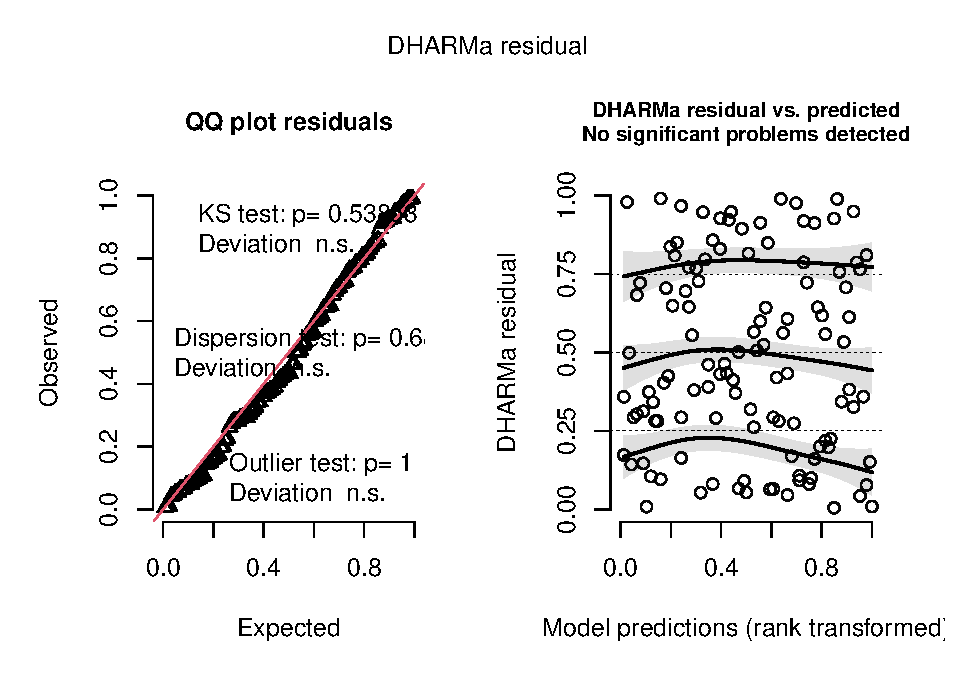
\includegraphics[keepaspectratio]{ch1_glm_clean_files/figure-latex/unnamed-chunk-21-1.pdf}}

\begin{enumerate}
\def\labelenumi{\arabic{enumi}.}
\setcounter{enumi}{2}
\tightlist
\item
  Look at results
\end{enumerate}

\begin{Shaded}
\begin{Highlighting}[]
\FunctionTok{summary}\NormalTok{(NSQ\_noRE)}
\end{Highlighting}
\end{Shaded}

\begin{verbatim}
##  Family: poisson  ( log )
## Formula:          
## nest_searching_queens ~ cover_type + bombus_floral_abun_scaled +  
##     num_burrows_scaled + prop_inactive_scaled + bee_season_type
## Zero inflation:                         
## ~cover_type + bombus_floral_abun_scaled + num_burrows_scaled + 
##     prop_inactive_scaled + bee_season_type
## Data: field_data
## 
##       AIC       BIC    logLik -2*log(L)  df.resid 
##     122.4     155.4     -49.2      98.4       104 
## 
## 
## Conditional model:
##                           Estimate Std. Error z value Pr(>|z|)   
## (Intercept)                -0.5946     0.4351  -1.367   0.1717   
## cover_typegrass             0.7957     0.4964   1.603   0.1090   
## bombus_floral_abun_scaled  -0.1537     0.2124  -0.724   0.4691   
## num_burrows_scaled          0.6810     0.3346   2.036   0.0418 * 
## prop_inactive_scaled       -0.4053     0.2592  -1.564   0.1179   
## bee_season_typeworker      -2.3731     0.7604  -3.121   0.0018 **
## ---
## Signif. codes:  0 '***' 0.001 '**' 0.01 '*' 0.05 '.' 0.1 ' ' 1
## 
## Zero-inflation model:
##                           Estimate Std. Error z value Pr(>|z|)
## (Intercept)                 -7.340      6.223  -1.180    0.238
## cover_typegrass            -22.434     17.284  -1.298    0.194
## bombus_floral_abun_scaled   -8.652      6.776  -1.277    0.202
## num_burrows_scaled          25.258     18.300   1.380    0.168
## prop_inactive_scaled       -38.354     28.059  -1.367    0.172
## bee_season_typeworker        1.863      3.655   0.510    0.610
\end{verbatim}

\subsection{Plots}\label{plots-3}

Number of nest-searching queens vs grass/forb

Conditional model:

\begin{Shaded}
\begin{Highlighting}[]
\CommentTok{\#create new data grid}
\NormalTok{nsq\_data\_cover}\OtherTok{\textless{}{-}} \FunctionTok{expand.grid}\NormalTok{(}
  \AttributeTok{cover\_type =} \FunctionTok{unique}\NormalTok{(field\_data}\SpecialCharTok{$}\NormalTok{cover\_type),}
  \AttributeTok{bombus\_floral\_abun\_scaled =} \FunctionTok{mean}\NormalTok{(field\_data}\SpecialCharTok{$}\NormalTok{bombus\_floral\_abun\_scaled, }\AttributeTok{na.rm =} \ConstantTok{TRUE}\NormalTok{),}
  \AttributeTok{num\_burrows\_scaled =} \FunctionTok{mean}\NormalTok{(field\_data}\SpecialCharTok{$}\NormalTok{num\_burrows\_scaled, }\AttributeTok{na.rm =} \ConstantTok{TRUE}\NormalTok{),}
  \AttributeTok{bee\_season\_type =} \StringTok{"nestsearching"}\NormalTok{,}
  \AttributeTok{prop\_inactive\_scaled =} \FunctionTok{mean}\NormalTok{(field\_data}\SpecialCharTok{$}\NormalTok{prop\_inactive\_scaled, }\AttributeTok{na.rm =} \ConstantTok{TRUE}\NormalTok{)}
\NormalTok{)}

\CommentTok{\# Predictions for conditional model (count)}
\NormalTok{pred\_nsq\_cover\_cond }\OtherTok{\textless{}{-}} \FunctionTok{predict}\NormalTok{(NSQ\_noRE,}
                            \AttributeTok{newdata =}\NormalTok{ nsq\_data\_cover,}
                            \AttributeTok{type =} \StringTok{"link"}\NormalTok{,}
                            \AttributeTok{se.fit =} \ConstantTok{TRUE}\NormalTok{)}

\CommentTok{\# Combine predictions with data frame}
\NormalTok{pred\_nsq\_cover\_df }\OtherTok{\textless{}{-}} \FunctionTok{cbind}\NormalTok{(nsq\_data\_cover,}
                 \AttributeTok{cond\_fit\_log =}\NormalTok{ pred\_nsq\_cover\_cond}\SpecialCharTok{$}\NormalTok{fit,}
                 \AttributeTok{cond\_se\_log =}\NormalTok{ pred\_nsq\_cover\_cond}\SpecialCharTok{$}\NormalTok{se.fit)}

\CommentTok{\#calculate predictions and confidence intervals on response scale (not log scale)}
\NormalTok{pred\_nsq\_cover\_df }\OtherTok{\textless{}{-}}\NormalTok{ pred\_nsq\_cover\_df }\SpecialCharTok{\%\textgreater{}\%}
  \FunctionTok{mutate}\NormalTok{(}
    \AttributeTok{cond\_fit =} \FunctionTok{exp}\NormalTok{(cond\_fit\_log),}
    \AttributeTok{cond\_lower =} \FunctionTok{exp}\NormalTok{(cond\_fit\_log }\SpecialCharTok{{-}} \FloatTok{1.96} \SpecialCharTok{*}\NormalTok{ cond\_se\_log),}
    \AttributeTok{cond\_upper =} \FunctionTok{exp}\NormalTok{(cond\_fit\_log }\SpecialCharTok{+} \FloatTok{1.96} \SpecialCharTok{*}\NormalTok{ cond\_se\_log)}
\NormalTok{  )}

\CommentTok{\#plot}
\FunctionTok{ggplot}\NormalTok{(pred\_nsq\_cover\_df, }\FunctionTok{aes}\NormalTok{(}\AttributeTok{x =}\NormalTok{ cover\_type, }\AttributeTok{y =}\NormalTok{ cond\_fit)) }\SpecialCharTok{+}
  \FunctionTok{geom\_point}\NormalTok{(}\AttributeTok{size =} \DecValTok{8}\NormalTok{) }\SpecialCharTok{+}
  \FunctionTok{geom\_errorbar}\NormalTok{(}\FunctionTok{aes}\NormalTok{(}\AttributeTok{ymin =}\NormalTok{ cond\_lower, }\AttributeTok{ymax =}\NormalTok{ cond\_upper), }\AttributeTok{width =} \FloatTok{0.2}\NormalTok{, }\AttributeTok{position =} \FunctionTok{position\_dodge}\NormalTok{(}\FloatTok{0.6}\NormalTok{), }\AttributeTok{linewidth =} \FloatTok{1.5}\NormalTok{) }\SpecialCharTok{+}
  \FunctionTok{labs}\NormalTok{(}
       \AttributeTok{x =} \StringTok{"Cover type"}\NormalTok{,}
       \AttributeTok{y =} \StringTok{"Predicted mean NSQ}\SpecialCharTok{\textbackslash{}n}\StringTok{count (per plot)"}\NormalTok{) }\SpecialCharTok{+}
  \FunctionTok{theme\_classic}\NormalTok{(}\AttributeTok{base\_size =} \DecValTok{23}\NormalTok{)}
\end{Highlighting}
\end{Shaded}

\pandocbounded{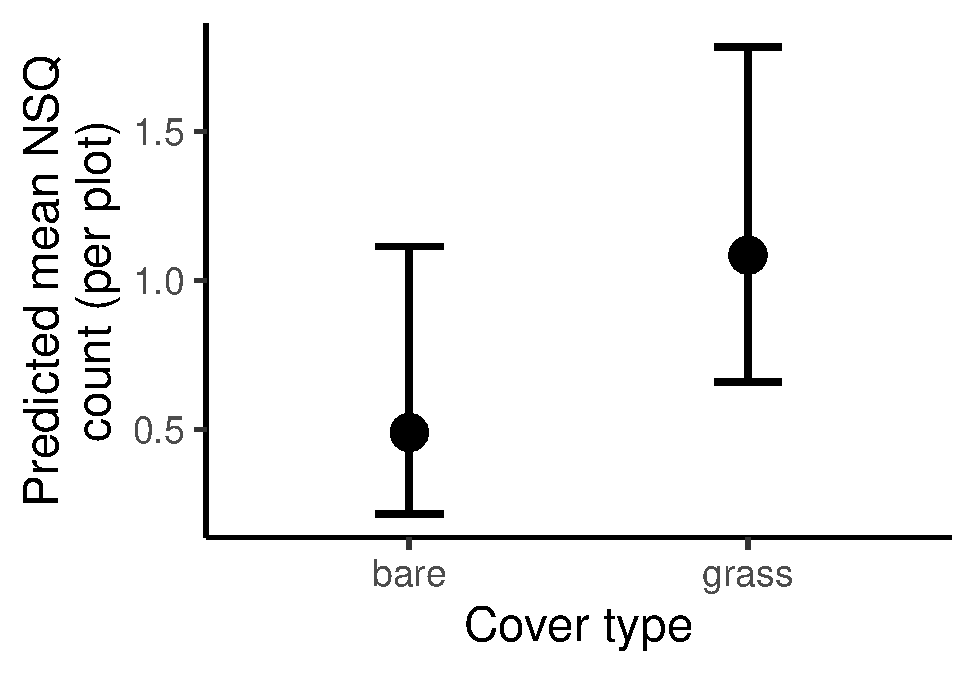
\includegraphics[keepaspectratio]{ch1_glm_clean_files/figure-latex/unnamed-chunk-23-1.pdf}}

Zero-inflated model:

\begin{Shaded}
\begin{Highlighting}[]
\CommentTok{\# Predictions for ZI model }
\NormalTok{pred\_nsq\_cover\_zi }\OtherTok{\textless{}{-}} \FunctionTok{predict}\NormalTok{(NSQ\_noRE, }
                                \AttributeTok{newdata =}\NormalTok{ nsq\_data\_cover, }
                                \AttributeTok{type =} \StringTok{"zlink"}\NormalTok{,}
                              \AttributeTok{se.fit =} \ConstantTok{TRUE}\NormalTok{)}

\CommentTok{\# Combine predictions and transform to response scale (by applying the inverse logit (plogit))}
\NormalTok{pred\_nsq\_cover\_df }\OtherTok{\textless{}{-}} \FunctionTok{cbind}\NormalTok{(}
\NormalTok{  nsq\_data\_cover,}
  \AttributeTok{zi\_fit =} \FunctionTok{plogis}\NormalTok{(pred\_nsq\_cover\_zi}\SpecialCharTok{$}\NormalTok{fit),}
  \AttributeTok{zi\_lower =} \FunctionTok{plogis}\NormalTok{(pred\_nsq\_cover\_zi}\SpecialCharTok{$}\NormalTok{fit }\SpecialCharTok{{-}} \FloatTok{1.96} \SpecialCharTok{*}\NormalTok{ pred\_nsq\_cover\_zi}\SpecialCharTok{$}\NormalTok{se.fit),}
  \AttributeTok{zi\_upper =} \FunctionTok{plogis}\NormalTok{(pred\_nsq\_cover\_zi}\SpecialCharTok{$}\NormalTok{fit }\SpecialCharTok{+} \FloatTok{1.96} \SpecialCharTok{*}\NormalTok{ pred\_nsq\_cover\_zi}\SpecialCharTok{$}\NormalTok{se.fit)}
\NormalTok{)}

\CommentTok{\# Plot zi predictions}
\FunctionTok{ggplot}\NormalTok{(pred\_nsq\_cover\_df, }\FunctionTok{aes}\NormalTok{(}\AttributeTok{x =}\NormalTok{ cover\_type, }\AttributeTok{y =}\NormalTok{ zi\_fit)) }\SpecialCharTok{+}
  \FunctionTok{geom\_point}\NormalTok{(}\AttributeTok{size =} \DecValTok{8}\NormalTok{) }\SpecialCharTok{+}
  \FunctionTok{geom\_errorbar}\NormalTok{(}\FunctionTok{aes}\NormalTok{(}\AttributeTok{ymin =}\NormalTok{ zi\_lower, }\AttributeTok{ymax =}\NormalTok{ zi\_upper), }\AttributeTok{width =} \FloatTok{0.2}\NormalTok{, }\AttributeTok{position =} \FunctionTok{position\_dodge}\NormalTok{(}\FloatTok{0.6}\NormalTok{), }\AttributeTok{linewidth =} \FloatTok{1.5}\NormalTok{) }\SpecialCharTok{+}
  \FunctionTok{labs}\NormalTok{( }\AttributeTok{x =} \StringTok{"Cover type"}\NormalTok{, }\AttributeTok{y =} \StringTok{"Predicted probability}\SpecialCharTok{\textbackslash{}n}\StringTok{of structural zeros"}\NormalTok{) }\SpecialCharTok{+}
  \FunctionTok{theme\_classic}\NormalTok{(}\AttributeTok{base\_size =} \DecValTok{23}\NormalTok{) }
\end{Highlighting}
\end{Shaded}

\pandocbounded{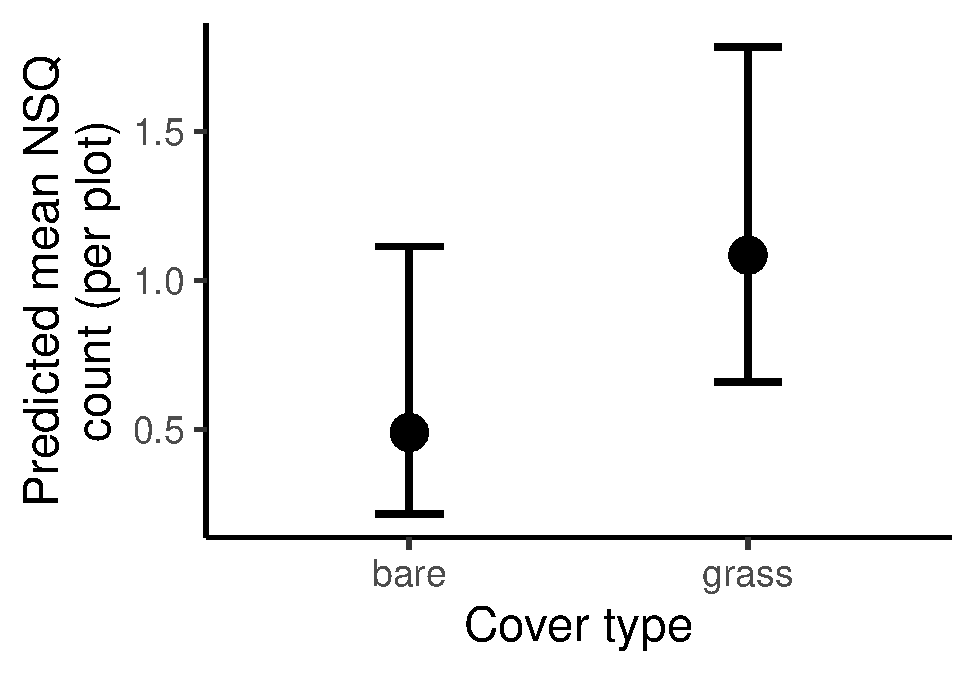
\includegraphics[keepaspectratio]{ch1_glm_clean_files/figure-latex/unnamed-chunk-24-1.pdf}}

Number of nest-searching queens vs floral abundance

Conditional model:

\begin{Shaded}
\begin{Highlighting}[]
\CommentTok{\# Define a sequence of values for bombus\_floral\_abun\_scaled across its observed range}
\NormalTok{floral\_seq }\OtherTok{\textless{}{-}} \FunctionTok{seq}\NormalTok{(}
  \AttributeTok{from =} \FunctionTok{min}\NormalTok{(field\_data}\SpecialCharTok{$}\NormalTok{bombus\_floral\_abun\_scaled, }\AttributeTok{na.rm =} \ConstantTok{TRUE}\NormalTok{),}
  \AttributeTok{to =} \FunctionTok{max}\NormalTok{(field\_data}\SpecialCharTok{$}\NormalTok{bombus\_floral\_abun\_scaled, }\AttributeTok{na.rm =} \ConstantTok{TRUE}\NormalTok{),}
  \AttributeTok{length.out =} \DecValTok{50}
\NormalTok{)}

\CommentTok{\# Create data grid over bombus\_floral\_abun\_scaled}
\NormalTok{nsq\_data\_floral }\OtherTok{\textless{}{-}} \FunctionTok{data.frame}\NormalTok{(}
  \AttributeTok{bombus\_floral\_abun\_scaled =}\NormalTok{ floral\_seq,}
  \AttributeTok{cover\_type =} \StringTok{"grass"}\NormalTok{,}
  \AttributeTok{num\_burrows\_scaled =} \FunctionTok{mean}\NormalTok{(field\_data}\SpecialCharTok{$}\NormalTok{num\_burrows\_scaled, }\AttributeTok{na.rm =} \ConstantTok{TRUE}\NormalTok{),}
  \AttributeTok{prop\_inactive\_scaled =} \FunctionTok{mean}\NormalTok{(field\_data}\SpecialCharTok{$}\NormalTok{prop\_inactive\_scaled, }\AttributeTok{na.rm =} \ConstantTok{TRUE}\NormalTok{),}
  \AttributeTok{bee\_season\_type =} \StringTok{"nestsearching"}  
\NormalTok{)}

\CommentTok{\# Predictions for conditional model (count)}
\NormalTok{pred\_nsq\_floral\_cond }\OtherTok{\textless{}{-}} \FunctionTok{predict}\NormalTok{(NSQ\_noRE, }
                                \AttributeTok{newdata =}\NormalTok{ nsq\_data\_floral, }
                                \AttributeTok{type =} \StringTok{"link"}\NormalTok{, }
                                \AttributeTok{se.fit =} \ConstantTok{TRUE}\NormalTok{)}

\CommentTok{\# Combine predictions with newdata}
\NormalTok{pred\_nsq\_floral\_df }\OtherTok{\textless{}{-}} \FunctionTok{cbind}\NormalTok{(nsq\_data\_floral,}
                 \AttributeTok{cond\_fit\_log =}\NormalTok{ pred\_nsq\_floral\_cond}\SpecialCharTok{$}\NormalTok{fit,}
                 \AttributeTok{cond\_se\_log =}\NormalTok{ pred\_nsq\_floral\_cond}\SpecialCharTok{$}\NormalTok{se.fit)}

\CommentTok{\#calculate predictions and confidence intervals on response scale (not log scale)}
\NormalTok{pred\_nsq\_floral\_df }\OtherTok{\textless{}{-}}\NormalTok{ pred\_nsq\_floral\_df }\SpecialCharTok{\%\textgreater{}\%}
  \FunctionTok{mutate}\NormalTok{(}
    \AttributeTok{cond\_fit =} \FunctionTok{exp}\NormalTok{(cond\_fit\_log),}
    \AttributeTok{cond\_lower =} \FunctionTok{exp}\NormalTok{(cond\_fit\_log }\SpecialCharTok{{-}} \FloatTok{1.96} \SpecialCharTok{*}\NormalTok{ cond\_se\_log),}
    \AttributeTok{cond\_upper =} \FunctionTok{exp}\NormalTok{(cond\_fit\_log }\SpecialCharTok{+} \FloatTok{1.96} \SpecialCharTok{*}\NormalTok{ cond\_se\_log)}
\NormalTok{  )}

\CommentTok{\# Plot conditional predictions}
\FunctionTok{ggplot}\NormalTok{(pred\_nsq\_floral\_df, }\FunctionTok{aes}\NormalTok{(}\AttributeTok{x =}\NormalTok{ bombus\_floral\_abun\_scaled, }\AttributeTok{y =}\NormalTok{ cond\_fit)) }\SpecialCharTok{+}
  \FunctionTok{geom\_line}\NormalTok{(}\AttributeTok{linewidth =} \DecValTok{3}\NormalTok{) }\SpecialCharTok{+}
  \FunctionTok{geom\_ribbon}\NormalTok{(}\FunctionTok{aes}\NormalTok{(}\AttributeTok{ymin =}\NormalTok{ cond\_lower, }\AttributeTok{ymax =}\NormalTok{ cond\_upper), }\AttributeTok{alpha =} \FloatTok{0.2}\NormalTok{) }\SpecialCharTok{+}
  \FunctionTok{labs}\NormalTok{( }\AttributeTok{x =} \StringTok{"Floral abundance (scaled)"}\NormalTok{ , }\AttributeTok{y =} \StringTok{"Predicted mean NSQ}\SpecialCharTok{\textbackslash{}n}\StringTok{count (per plot)"}\NormalTok{) }\SpecialCharTok{+}
  \FunctionTok{theme\_classic}\NormalTok{(}\AttributeTok{base\_size =} \DecValTok{23}\NormalTok{)}
\end{Highlighting}
\end{Shaded}

\pandocbounded{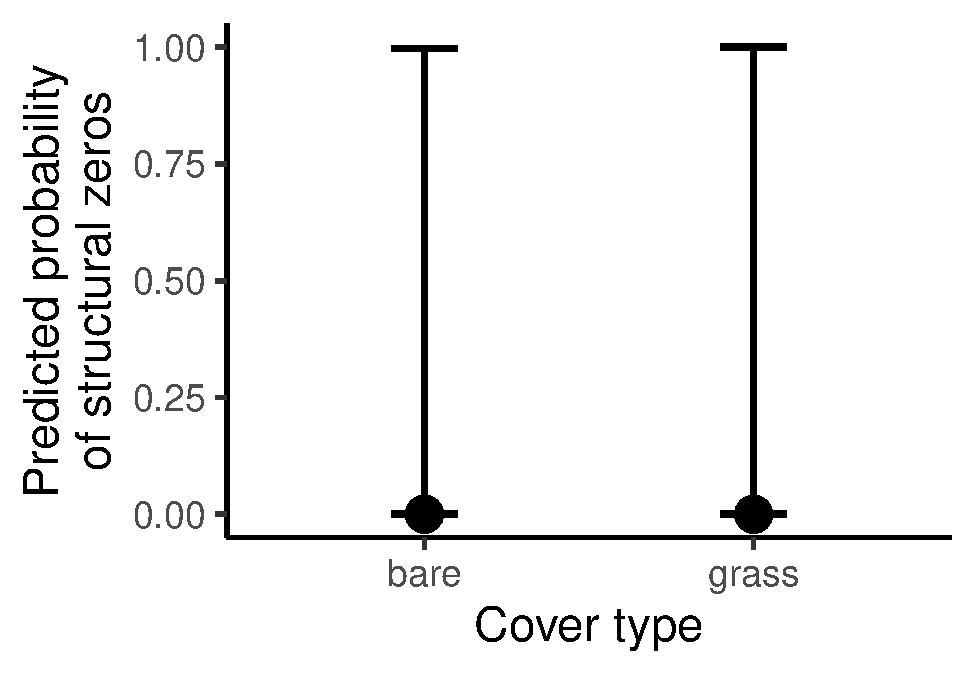
\includegraphics[keepaspectratio]{ch1_glm_clean_files/figure-latex/unnamed-chunk-25-1.pdf}}

Zero-inflated model:

\begin{Shaded}
\begin{Highlighting}[]
\CommentTok{\# Predictions for ZI model }
\NormalTok{pred\_nsq\_floral\_zi }\OtherTok{\textless{}{-}} \FunctionTok{predict}\NormalTok{(NSQ\_noRE, }
                                \AttributeTok{newdata =}\NormalTok{ nsq\_data\_floral, }
                                \AttributeTok{type =} \StringTok{"zlink"}\NormalTok{,}
                              \AttributeTok{se.fit =} \ConstantTok{TRUE}\NormalTok{)}

\CommentTok{\# Combine predictions and transform to response scale (by applying the inverse logit (plogit))}
\NormalTok{pred\_nsq\_floral\_df }\OtherTok{\textless{}{-}} \FunctionTok{cbind}\NormalTok{(}
\NormalTok{  nsq\_data\_floral,}
  \AttributeTok{zi\_fit =} \FunctionTok{plogis}\NormalTok{(pred\_nsq\_floral\_zi}\SpecialCharTok{$}\NormalTok{fit),}
  \AttributeTok{zi\_lower =} \FunctionTok{plogis}\NormalTok{(pred\_nsq\_floral\_zi}\SpecialCharTok{$}\NormalTok{fit }\SpecialCharTok{{-}} \FloatTok{1.96} \SpecialCharTok{*}\NormalTok{ pred\_nsq\_floral\_zi}\SpecialCharTok{$}\NormalTok{se.fit),}
  \AttributeTok{zi\_upper =} \FunctionTok{plogis}\NormalTok{(pred\_nsq\_floral\_zi}\SpecialCharTok{$}\NormalTok{fit }\SpecialCharTok{+} \FloatTok{1.96} \SpecialCharTok{*}\NormalTok{ pred\_nsq\_floral\_zi}\SpecialCharTok{$}\NormalTok{se.fit)}
\NormalTok{)}

\CommentTok{\# Plot zi predictions}
\FunctionTok{ggplot}\NormalTok{(pred\_nsq\_floral\_df, }\FunctionTok{aes}\NormalTok{(}\AttributeTok{x =}\NormalTok{ bombus\_floral\_abun\_scaled, }\AttributeTok{y =}\NormalTok{ zi\_fit)) }\SpecialCharTok{+}
  \FunctionTok{geom\_line}\NormalTok{(}\AttributeTok{linewidth =} \DecValTok{3}\NormalTok{) }\SpecialCharTok{+}
  \FunctionTok{geom\_ribbon}\NormalTok{(}\FunctionTok{aes}\NormalTok{(}\AttributeTok{ymin =}\NormalTok{ zi\_lower, }\AttributeTok{ymax =}\NormalTok{ zi\_upper), }\AttributeTok{alpha =} \FloatTok{0.2}\NormalTok{) }\SpecialCharTok{+}
  \FunctionTok{labs}\NormalTok{(}\AttributeTok{x =} \StringTok{"Floral abundance (scaled)"}\NormalTok{, }\AttributeTok{y =} \StringTok{"Predicted probability}\SpecialCharTok{\textbackslash{}n}\StringTok{of structural zeros"}\NormalTok{) }\SpecialCharTok{+}
  \FunctionTok{theme\_classic}\NormalTok{(}\AttributeTok{base\_size =} \DecValTok{23}\NormalTok{)}
\end{Highlighting}
\end{Shaded}

\pandocbounded{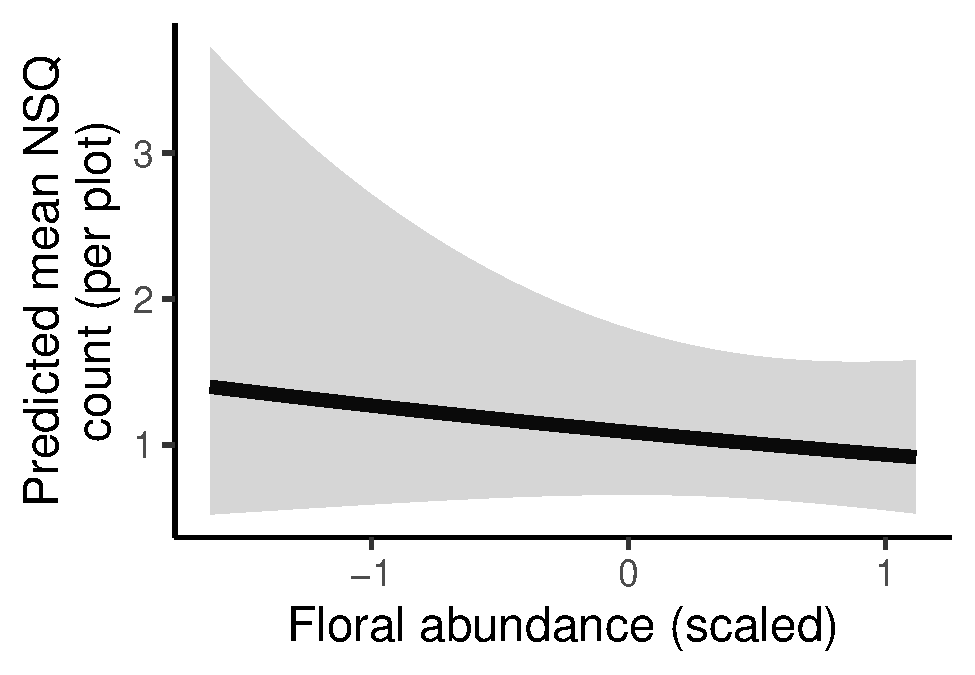
\includegraphics[keepaspectratio]{ch1_glm_clean_files/figure-latex/unnamed-chunk-26-1.pdf}}

Number of nest-searching queens vs burrow vacancy proportion

Conditional model:

\begin{Shaded}
\begin{Highlighting}[]
\CommentTok{\#create new data grid}
\NormalTok{nsq\_data\_vacancy}\OtherTok{\textless{}{-}} \FunctionTok{expand.grid}\NormalTok{(}
  \AttributeTok{cover\_type =} \StringTok{"grass"}\NormalTok{,}
  \AttributeTok{bombus\_floral\_abun\_scaled =} \FunctionTok{mean}\NormalTok{(field\_data}\SpecialCharTok{$}\NormalTok{bombus\_floral\_abun\_scaled, }\AttributeTok{na.rm =} \ConstantTok{TRUE}\NormalTok{),}
  \AttributeTok{num\_burrows\_scaled =} \FunctionTok{mean}\NormalTok{(field\_data}\SpecialCharTok{$}\NormalTok{num\_burrows\_scaled, }\AttributeTok{na.rm =} \ConstantTok{TRUE}\NormalTok{),}
  \AttributeTok{bee\_season\_type =} \StringTok{"nestsearching"}\NormalTok{,}
  \AttributeTok{prop\_inactive\_scaled =} \FunctionTok{seq}\NormalTok{(}\FunctionTok{min}\NormalTok{(field\_data}\SpecialCharTok{$}\NormalTok{prop\_inactive\_scaled, }\AttributeTok{na.rm =} \ConstantTok{TRUE}\NormalTok{), }
                             \FunctionTok{max}\NormalTok{(field\_data}\SpecialCharTok{$}\NormalTok{prop\_inactive\_scaled, }\AttributeTok{na.rm =} \ConstantTok{TRUE}\NormalTok{), }
                             \AttributeTok{length.out =} \DecValTok{50}\NormalTok{)}
\NormalTok{)}

\CommentTok{\# Predictions for conditional model (count)}
\NormalTok{pred\_nsq\_vacancy\_cond }\OtherTok{\textless{}{-}} \FunctionTok{predict}\NormalTok{(NSQ\_noRE,}
                            \AttributeTok{newdata =}\NormalTok{ nsq\_data\_vacancy,}
                            \AttributeTok{type =} \StringTok{"link"}\NormalTok{,}
                            \AttributeTok{se.fit =} \ConstantTok{TRUE}\NormalTok{)}

\CommentTok{\# Combine predictions with data frame}
\NormalTok{pred\_nsq\_vacancy\_df }\OtherTok{\textless{}{-}} \FunctionTok{cbind}\NormalTok{(nsq\_data\_vacancy,}
                 \AttributeTok{cond\_fit\_log =}\NormalTok{ pred\_nsq\_vacancy\_cond}\SpecialCharTok{$}\NormalTok{fit,}
                 \AttributeTok{cond\_se\_log =}\NormalTok{ pred\_nsq\_vacancy\_cond}\SpecialCharTok{$}\NormalTok{se.fit)}

\CommentTok{\#calculate predictions and confidence intervals on response scale (not log scale)}
\NormalTok{pred\_nsq\_vacancy\_df }\OtherTok{\textless{}{-}}\NormalTok{ pred\_nsq\_vacancy\_df }\SpecialCharTok{\%\textgreater{}\%}
  \FunctionTok{mutate}\NormalTok{(}
    \AttributeTok{cond\_fit =} \FunctionTok{exp}\NormalTok{(cond\_fit\_log),}
    \AttributeTok{cond\_lower =} \FunctionTok{exp}\NormalTok{(cond\_fit\_log }\SpecialCharTok{{-}} \FloatTok{1.96} \SpecialCharTok{*}\NormalTok{ cond\_se\_log),}
    \AttributeTok{cond\_upper =} \FunctionTok{exp}\NormalTok{(cond\_fit\_log }\SpecialCharTok{+} \FloatTok{1.96} \SpecialCharTok{*}\NormalTok{ cond\_se\_log)}
\NormalTok{  )}

\CommentTok{\#plot}
\FunctionTok{ggplot}\NormalTok{(pred\_nsq\_vacancy\_df, }\FunctionTok{aes}\NormalTok{(}\AttributeTok{x =}\NormalTok{ prop\_inactive\_scaled, }\AttributeTok{y =}\NormalTok{ cond\_fit)) }\SpecialCharTok{+}
  \FunctionTok{geom\_line}\NormalTok{(}\AttributeTok{linewidth =} \DecValTok{3}\NormalTok{) }\SpecialCharTok{+}
  \FunctionTok{geom\_ribbon}\NormalTok{(}\FunctionTok{aes}\NormalTok{(}\AttributeTok{ymin =}\NormalTok{ cond\_lower, }\AttributeTok{ymax =}\NormalTok{ cond\_upper), }\AttributeTok{alpha =} \FloatTok{0.2}\NormalTok{) }\SpecialCharTok{+}
  \FunctionTok{labs}\NormalTok{(}
       \AttributeTok{x =} \StringTok{"Proportion of vacant burrows (scaled)"}\NormalTok{,}
       \AttributeTok{y =} \StringTok{"Predicted mean NSQ}\SpecialCharTok{\textbackslash{}n}\StringTok{count (per plot)"}\NormalTok{) }\SpecialCharTok{+}
  \FunctionTok{theme\_classic}\NormalTok{(}\AttributeTok{base\_size =} \DecValTok{23}\NormalTok{)}
\end{Highlighting}
\end{Shaded}

\pandocbounded{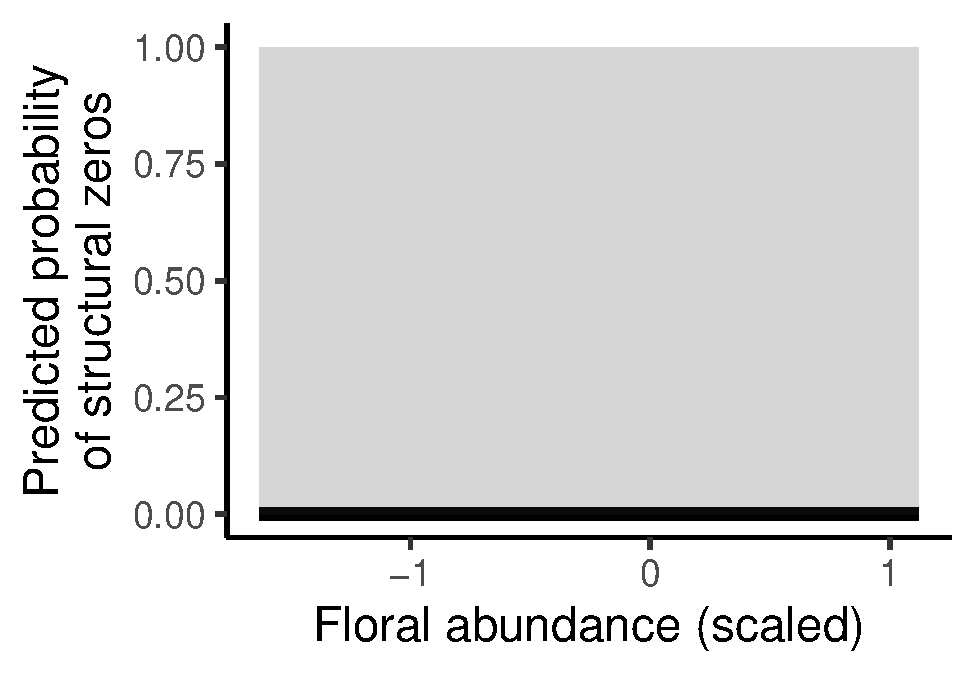
\includegraphics[keepaspectratio]{ch1_glm_clean_files/figure-latex/unnamed-chunk-27-1.pdf}}

Zero-inflated model:

\begin{Shaded}
\begin{Highlighting}[]
\CommentTok{\# Predictions for ZI model }
\NormalTok{pred\_nsq\_vacancy\_zi }\OtherTok{\textless{}{-}} \FunctionTok{predict}\NormalTok{(NSQ\_noRE, }
                                \AttributeTok{newdata =}\NormalTok{ nsq\_data\_vacancy, }
                                \AttributeTok{type =} \StringTok{"zlink"}\NormalTok{,}
                              \AttributeTok{se.fit =} \ConstantTok{TRUE}\NormalTok{)}

\CommentTok{\# Combine predictions and transform to response scale (by applying the inverse logit (plogit))}
\NormalTok{pred\_nsq\_vacancy\_df }\OtherTok{\textless{}{-}} \FunctionTok{cbind}\NormalTok{(}
\NormalTok{  nsq\_data\_vacancy,}
  \AttributeTok{zi\_fit =} \FunctionTok{plogis}\NormalTok{(pred\_nsq\_vacancy\_zi}\SpecialCharTok{$}\NormalTok{fit),}
  \AttributeTok{zi\_lower =} \FunctionTok{plogis}\NormalTok{(pred\_nsq\_vacancy\_zi}\SpecialCharTok{$}\NormalTok{fit }\SpecialCharTok{{-}} \FloatTok{1.96} \SpecialCharTok{*}\NormalTok{ pred\_nsq\_vacancy\_zi}\SpecialCharTok{$}\NormalTok{se.fit),}
  \AttributeTok{zi\_upper =} \FunctionTok{plogis}\NormalTok{(pred\_nsq\_vacancy\_zi}\SpecialCharTok{$}\NormalTok{fit }\SpecialCharTok{+} \FloatTok{1.96} \SpecialCharTok{*}\NormalTok{ pred\_nsq\_vacancy\_zi}\SpecialCharTok{$}\NormalTok{se.fit)}
\NormalTok{)}

\CommentTok{\# Plot zi predictions}
\FunctionTok{ggplot}\NormalTok{(pred\_nsq\_vacancy\_df, }\FunctionTok{aes}\NormalTok{(}\AttributeTok{x =}\NormalTok{ prop\_inactive\_scaled, }\AttributeTok{y =}\NormalTok{ zi\_fit)) }\SpecialCharTok{+}
  \FunctionTok{geom\_line}\NormalTok{(}\AttributeTok{linewidth =} \DecValTok{3}\NormalTok{) }\SpecialCharTok{+}
  \FunctionTok{geom\_ribbon}\NormalTok{(}\FunctionTok{aes}\NormalTok{(}\AttributeTok{ymin =}\NormalTok{ zi\_lower, }\AttributeTok{ymax =}\NormalTok{ zi\_upper), }\AttributeTok{alpha =} \FloatTok{0.2}\NormalTok{) }\SpecialCharTok{+}
  \FunctionTok{labs}\NormalTok{( }\AttributeTok{x =} \StringTok{"Proportion of vacant burrows (scaled)"}\NormalTok{, }\AttributeTok{y =} \StringTok{"Predicted probability}\SpecialCharTok{\textbackslash{}n}\StringTok{of structural zeros"}\NormalTok{) }\SpecialCharTok{+}
  \FunctionTok{theme\_classic}\NormalTok{(}\AttributeTok{base\_size =} \DecValTok{23}\NormalTok{) }
\end{Highlighting}
\end{Shaded}

\pandocbounded{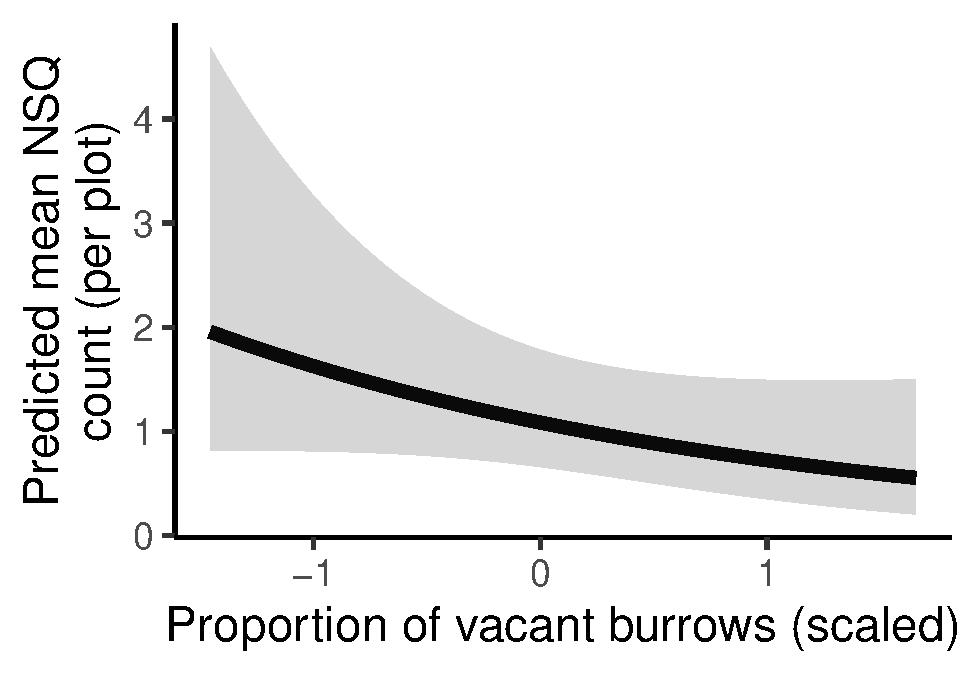
\includegraphics[keepaspectratio]{ch1_glm_clean_files/figure-latex/unnamed-chunk-28-1.pdf}}

Number of nest-searching queens vs number of rodent burrows

Conditional model:

\begin{Shaded}
\begin{Highlighting}[]
\CommentTok{\# Create data grid over rodent\_burrows\_scaled}
\NormalTok{nsq\_data\_rodent }\OtherTok{\textless{}{-}} \FunctionTok{data.frame}\NormalTok{(}
  \AttributeTok{num\_burrows\_scaled =} \FunctionTok{seq}\NormalTok{(}\FunctionTok{min}\NormalTok{(field\_data}\SpecialCharTok{$}\NormalTok{num\_burrows\_scaled), }\FunctionTok{max}\NormalTok{(field\_data}\SpecialCharTok{$}\NormalTok{num\_burrows\_scaled), }\AttributeTok{length.out =} \DecValTok{50}\NormalTok{),}
  \AttributeTok{prop\_inactive\_scaled =} \FunctionTok{mean}\NormalTok{(field\_data}\SpecialCharTok{$}\NormalTok{prop\_inactive\_scaled, }\AttributeTok{na.rm =} \ConstantTok{TRUE}\NormalTok{),}
  \AttributeTok{cover\_type =} \StringTok{"grass"}\NormalTok{,}
  \AttributeTok{bombus\_floral\_abun\_scaled =} \FunctionTok{mean}\NormalTok{(field\_data}\SpecialCharTok{$}\NormalTok{bombus\_floral\_abun\_scaled, }\AttributeTok{na.rm =} \ConstantTok{TRUE}\NormalTok{),}
  \AttributeTok{bee\_season\_type =} \StringTok{"nestsearching"}  
\NormalTok{)}

\CommentTok{\# Predictions for conditional model (count)}
\NormalTok{pred\_nsq\_rodent\_cond }\OtherTok{\textless{}{-}} \FunctionTok{predict}\NormalTok{(}
\NormalTok{  NSQ\_noRE, }
  \AttributeTok{newdata =}\NormalTok{ nsq\_data\_rodent, }
  \AttributeTok{type =} \StringTok{"link"}\NormalTok{, }\DocumentationTok{\#\#log{-}scale}
  \AttributeTok{se.fit =} \ConstantTok{TRUE}\NormalTok{)}

\CommentTok{\# Combine predictions with newdata}
\NormalTok{pred\_nsq\_rodent\_df }\OtherTok{\textless{}{-}} \FunctionTok{cbind}\NormalTok{(nsq\_data\_rodent,}
                 \AttributeTok{cond\_fit\_log =}\NormalTok{ pred\_nsq\_rodent\_cond}\SpecialCharTok{$}\NormalTok{fit,}
                 \AttributeTok{cond\_se\_log =}\NormalTok{ pred\_nsq\_rodent\_cond}\SpecialCharTok{$}\NormalTok{se.fit)}

\CommentTok{\#calculate predictions and confidence intervals on response scale (not log scale)}
\NormalTok{pred\_nsq\_rodent\_df }\OtherTok{\textless{}{-}}\NormalTok{ pred\_nsq\_rodent\_df }\SpecialCharTok{\%\textgreater{}\%}
  \FunctionTok{mutate}\NormalTok{(}
    \AttributeTok{cond\_fit =} \FunctionTok{exp}\NormalTok{(cond\_fit\_log),}
    \AttributeTok{cond\_lower =} \FunctionTok{exp}\NormalTok{(cond\_fit\_log }\SpecialCharTok{{-}} \FloatTok{1.96} \SpecialCharTok{*}\NormalTok{ cond\_se\_log),}
    \AttributeTok{cond\_upper =} \FunctionTok{exp}\NormalTok{(cond\_fit\_log }\SpecialCharTok{+} \FloatTok{1.96} \SpecialCharTok{*}\NormalTok{ cond\_se\_log)}
\NormalTok{  )}

\FunctionTok{ggplot}\NormalTok{(pred\_nsq\_rodent\_df, }\FunctionTok{aes}\NormalTok{(}\AttributeTok{x =}\NormalTok{ num\_burrows\_scaled, }\AttributeTok{y =}\NormalTok{ cond\_fit)) }\SpecialCharTok{+}
  \FunctionTok{geom\_line}\NormalTok{(}\AttributeTok{size =} \DecValTok{3}\NormalTok{) }\SpecialCharTok{+}
  \FunctionTok{geom\_ribbon}\NormalTok{(}\FunctionTok{aes}\NormalTok{(}\AttributeTok{ymin =}\NormalTok{ cond\_lower, }\AttributeTok{ymax =}\NormalTok{ cond\_upper), }\AttributeTok{alpha =} \FloatTok{0.2}\NormalTok{) }\SpecialCharTok{+}
  \FunctionTok{labs}\NormalTok{(}
    \AttributeTok{x =} \StringTok{"Burrow abundance (scaled)"}\NormalTok{,}
    \AttributeTok{y =} \StringTok{"Predicted mean NSQ}\SpecialCharTok{\textbackslash{}n}\StringTok{count (per plot)"}
\NormalTok{  ) }\SpecialCharTok{+}
  \FunctionTok{theme\_classic}\NormalTok{(}\AttributeTok{base\_size =} \DecValTok{23}\NormalTok{)}
\end{Highlighting}
\end{Shaded}

\begin{verbatim}
## Warning: Using `size` aesthetic for lines was deprecated in ggplot2 3.4.0.
## i Please use `linewidth` instead.
## This warning is displayed once every 8 hours.
## Call `lifecycle::last_lifecycle_warnings()` to see where this warning was
## generated.
\end{verbatim}

\pandocbounded{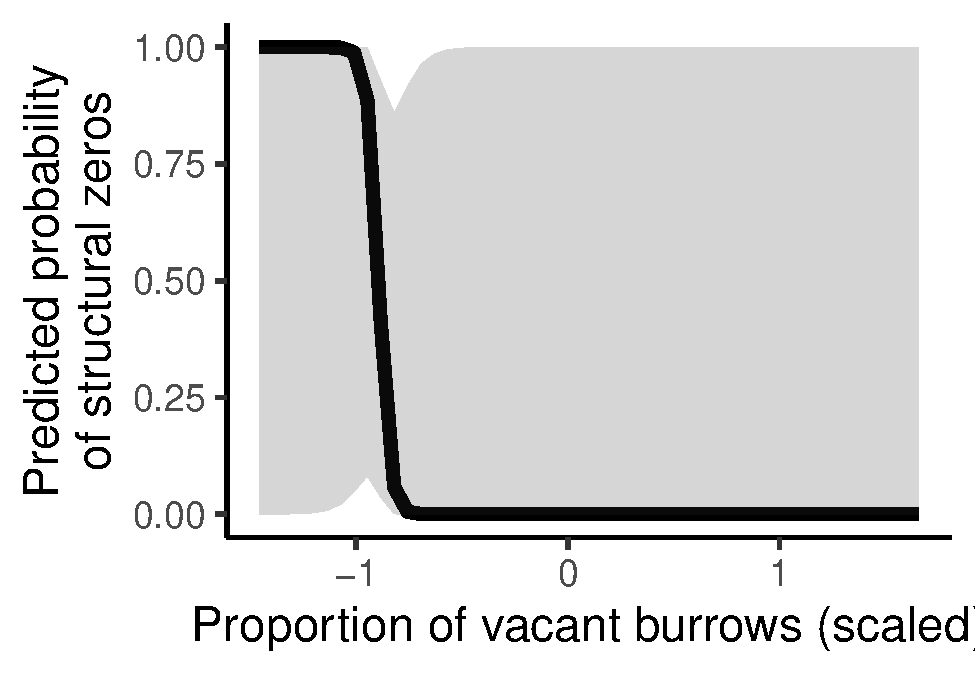
\includegraphics[keepaspectratio]{ch1_glm_clean_files/figure-latex/unnamed-chunk-29-1.pdf}}

Zero-inflated model:

\begin{Shaded}
\begin{Highlighting}[]
\CommentTok{\# Predictions for ZI model }
\NormalTok{pred\_nsq\_rodent\_zi }\OtherTok{\textless{}{-}} \FunctionTok{predict}\NormalTok{(NSQ\_noRE, }
                                \AttributeTok{newdata =}\NormalTok{ nsq\_data\_rodent, }
                                \AttributeTok{type =} \StringTok{"zlink"}\NormalTok{,}
                              \AttributeTok{se.fit =} \ConstantTok{TRUE}\NormalTok{)}

\CommentTok{\# Combine predictions and transform to response scale (by applying the inverse logit (plogit))}
\NormalTok{pred\_nsq\_rodent\_df }\OtherTok{\textless{}{-}} \FunctionTok{cbind}\NormalTok{(}
\NormalTok{  nsq\_data\_rodent,}
  \AttributeTok{zi\_fit =} \FunctionTok{plogis}\NormalTok{(pred\_nsq\_rodent\_zi}\SpecialCharTok{$}\NormalTok{fit),}
  \AttributeTok{zi\_lower =} \FunctionTok{plogis}\NormalTok{(pred\_nsq\_rodent\_zi}\SpecialCharTok{$}\NormalTok{fit }\SpecialCharTok{{-}} \FloatTok{1.96} \SpecialCharTok{*}\NormalTok{ pred\_nsq\_rodent\_zi}\SpecialCharTok{$}\NormalTok{se.fit),}
  \AttributeTok{zi\_upper =} \FunctionTok{plogis}\NormalTok{(pred\_nsq\_rodent\_zi}\SpecialCharTok{$}\NormalTok{fit }\SpecialCharTok{+} \FloatTok{1.96} \SpecialCharTok{*}\NormalTok{ pred\_nsq\_rodent\_zi}\SpecialCharTok{$}\NormalTok{se.fit)}
\NormalTok{)}

\FunctionTok{ggplot}\NormalTok{(pred\_nsq\_rodent\_df, }\FunctionTok{aes}\NormalTok{(}\AttributeTok{x =}\NormalTok{ num\_burrows\_scaled, }\AttributeTok{y =}\NormalTok{ zi\_fit)) }\SpecialCharTok{+}
  \FunctionTok{geom\_line}\NormalTok{(}\AttributeTok{size =} \DecValTok{3}\NormalTok{) }\SpecialCharTok{+}
  \FunctionTok{geom\_ribbon}\NormalTok{(}\FunctionTok{aes}\NormalTok{(}\AttributeTok{ymin =}\NormalTok{ zi\_lower, }\AttributeTok{ymax =}\NormalTok{ zi\_upper), }\AttributeTok{alpha =} \FloatTok{0.2}\NormalTok{) }\SpecialCharTok{+}
  \FunctionTok{labs}\NormalTok{(}\AttributeTok{x =} \StringTok{"Burrow abundance (scaled)"}\NormalTok{, }\AttributeTok{y =} \StringTok{"Predicted probability}\SpecialCharTok{\textbackslash{}n}\StringTok{of structural zeros"}\NormalTok{) }\SpecialCharTok{+}
  \FunctionTok{theme\_classic}\NormalTok{(}\AttributeTok{base\_size =} \DecValTok{23}\NormalTok{)}
\end{Highlighting}
\end{Shaded}

\pandocbounded{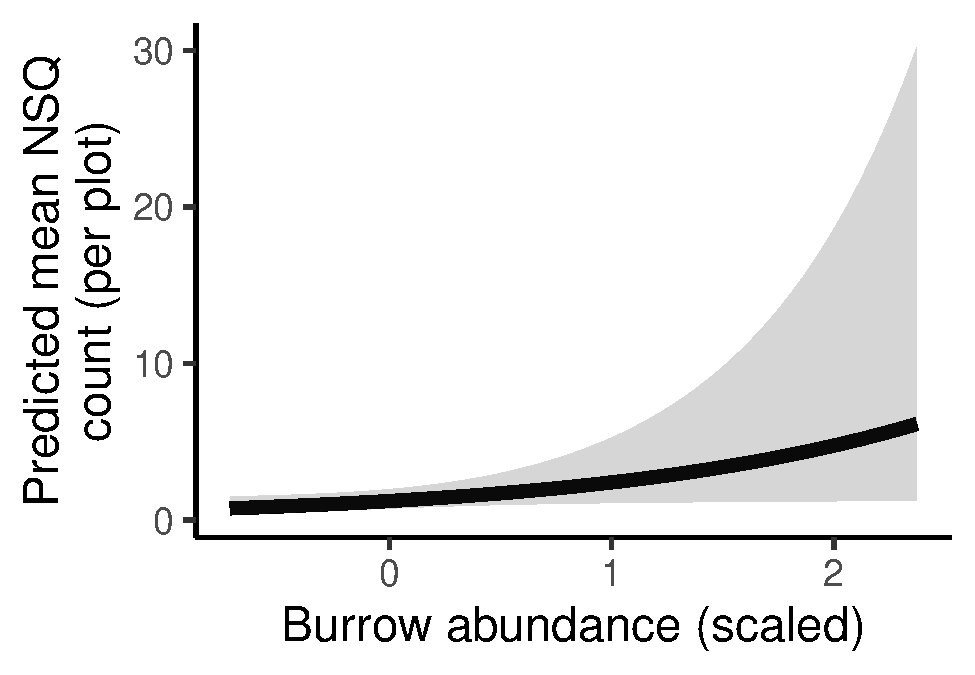
\includegraphics[keepaspectratio]{ch1_glm_clean_files/figure-latex/unnamed-chunk-30-1.pdf}}

Number of nest-searching queens vs season type

Conditional model:

\begin{Shaded}
\begin{Highlighting}[]
\CommentTok{\# Create newdata with discrete factor levels for bee\_season\_type}
\NormalTok{nsq\_data\_season }\OtherTok{\textless{}{-}} \FunctionTok{data.frame}\NormalTok{(}
  \AttributeTok{cover\_type =} \StringTok{"grass"}\NormalTok{,}
  \AttributeTok{bombus\_floral\_abun\_scaled =} \FunctionTok{mean}\NormalTok{(field\_data}\SpecialCharTok{$}\NormalTok{bombus\_floral\_abun\_scaled),}
  \AttributeTok{num\_burrows\_scaled =} \FunctionTok{mean}\NormalTok{(field\_data}\SpecialCharTok{$}\NormalTok{num\_burrows\_scaled, }\AttributeTok{na.rm =} \ConstantTok{TRUE}\NormalTok{),}
  \AttributeTok{prop\_inactive\_scaled =} \FunctionTok{mean}\NormalTok{(field\_data}\SpecialCharTok{$}\NormalTok{prop\_inactive\_scaled, }\AttributeTok{na.rm =} \ConstantTok{TRUE}\NormalTok{),}
  \AttributeTok{bee\_season\_type =} \FunctionTok{factor}\NormalTok{(}\FunctionTok{c}\NormalTok{(}\StringTok{"nestsearching"}\NormalTok{, }\StringTok{"worker"}\NormalTok{), }\AttributeTok{levels =} \FunctionTok{levels}\NormalTok{(field\_data}\SpecialCharTok{$}\NormalTok{bee\_season\_type))}
\NormalTok{)}

\CommentTok{\# Predictions for conditional model (count)}
\NormalTok{pred\_nsq\_season\_cond }\OtherTok{\textless{}{-}} \FunctionTok{predict}\NormalTok{(}
\NormalTok{  NSQ\_noRE, }
  \AttributeTok{newdata =}\NormalTok{ nsq\_data\_season, }
  \AttributeTok{type =} \StringTok{"link"}\NormalTok{, }\DocumentationTok{\#\#log{-}scale}
  \AttributeTok{se.fit =} \ConstantTok{TRUE}\NormalTok{)}

\CommentTok{\# Combine predictions with newdata}
\NormalTok{pred\_nsq\_season\_df }\OtherTok{\textless{}{-}} \FunctionTok{cbind}\NormalTok{(nsq\_data\_season,}
                 \AttributeTok{cond\_fit\_log =}\NormalTok{ pred\_nsq\_season\_cond}\SpecialCharTok{$}\NormalTok{fit,}
                 \AttributeTok{cond\_se\_log =}\NormalTok{ pred\_nsq\_season\_cond}\SpecialCharTok{$}\NormalTok{se.fit)}

\CommentTok{\#calculate predictions and confidence intervals on response scale (not log scale)}
\NormalTok{pred\_nsq\_season\_df }\OtherTok{\textless{}{-}}\NormalTok{ pred\_nsq\_season\_df }\SpecialCharTok{\%\textgreater{}\%}
  \FunctionTok{mutate}\NormalTok{(}
    \AttributeTok{cond\_fit =} \FunctionTok{exp}\NormalTok{(cond\_fit\_log),}
    \AttributeTok{cond\_lower =} \FunctionTok{exp}\NormalTok{(cond\_fit\_log }\SpecialCharTok{{-}} \FloatTok{1.96} \SpecialCharTok{*}\NormalTok{ cond\_se\_log),}
    \AttributeTok{cond\_upper =} \FunctionTok{exp}\NormalTok{(cond\_fit\_log }\SpecialCharTok{+} \FloatTok{1.96} \SpecialCharTok{*}\NormalTok{ cond\_se\_log)}
\NormalTok{  )}

\CommentTok{\# Plot conditional predictions}
\FunctionTok{ggplot}\NormalTok{(pred\_nsq\_season\_df, }\FunctionTok{aes}\NormalTok{(}\AttributeTok{x =}\NormalTok{ bee\_season\_type, }\AttributeTok{y =}\NormalTok{ cond\_fit)) }\SpecialCharTok{+}
  \FunctionTok{geom\_point}\NormalTok{(}\AttributeTok{size=}\DecValTok{8}\NormalTok{) }\SpecialCharTok{+}
  \FunctionTok{geom\_errorbar}\NormalTok{(}\FunctionTok{aes}\NormalTok{(}\AttributeTok{ymin =}\NormalTok{ cond\_lower, }\AttributeTok{ymax =}\NormalTok{ cond\_upper), }\AttributeTok{width =} \FloatTok{0.2}\NormalTok{, }\AttributeTok{position =} \FunctionTok{position\_dodge}\NormalTok{(}\FloatTok{0.6}\NormalTok{), }\AttributeTok{linewidth =} \FloatTok{1.5}\NormalTok{)}\SpecialCharTok{+}
  \FunctionTok{labs}\NormalTok{(}\AttributeTok{x =} \StringTok{"Bee season"}\NormalTok{, }\AttributeTok{y =} \StringTok{"Predicted mean NSQ}\SpecialCharTok{\textbackslash{}n}\StringTok{count (per plot)"}\NormalTok{) }\SpecialCharTok{+}
  \FunctionTok{theme\_classic}\NormalTok{(}\AttributeTok{base\_size =} \DecValTok{23}\NormalTok{)}
\end{Highlighting}
\end{Shaded}

\pandocbounded{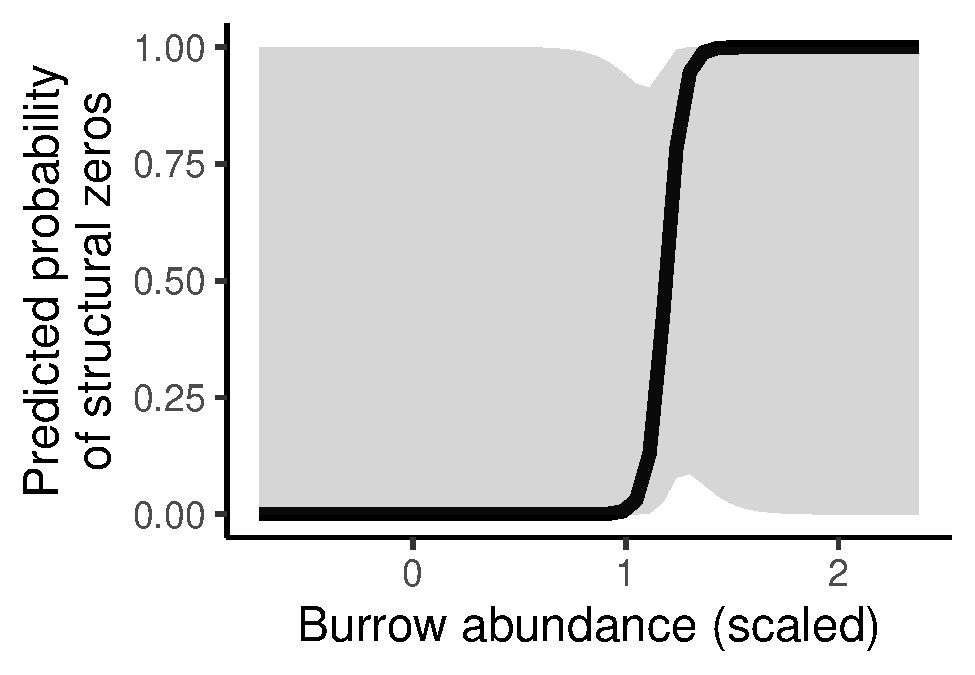
\includegraphics[keepaspectratio]{ch1_glm_clean_files/figure-latex/unnamed-chunk-31-1.pdf}}

Zero-inflated model:

\begin{Shaded}
\begin{Highlighting}[]
\CommentTok{\# Predictions for ZI model }
\NormalTok{pred\_nsq\_season\_zi }\OtherTok{\textless{}{-}} \FunctionTok{predict}\NormalTok{(NSQ\_noRE, }
                                \AttributeTok{newdata =}\NormalTok{ nsq\_data\_season, }
                                \AttributeTok{type =} \StringTok{"zlink"}\NormalTok{,}
                              \AttributeTok{se.fit =} \ConstantTok{TRUE}\NormalTok{)}

\CommentTok{\# Combine predictions and transform to response scale (by applying the inverse logit (plogit))}
\NormalTok{pred\_nsq\_season\_df }\OtherTok{\textless{}{-}} \FunctionTok{cbind}\NormalTok{(}
\NormalTok{  nsq\_data\_season,}
  \AttributeTok{zi\_fit =} \FunctionTok{plogis}\NormalTok{(pred\_nsq\_season\_zi}\SpecialCharTok{$}\NormalTok{fit),}
  \AttributeTok{zi\_lower =} \FunctionTok{plogis}\NormalTok{(pred\_nsq\_season\_zi}\SpecialCharTok{$}\NormalTok{fit }\SpecialCharTok{{-}} \FloatTok{1.96} \SpecialCharTok{*}\NormalTok{ pred\_nsq\_season\_zi}\SpecialCharTok{$}\NormalTok{se.fit),}
  \AttributeTok{zi\_upper =} \FunctionTok{plogis}\NormalTok{(pred\_nsq\_season\_zi}\SpecialCharTok{$}\NormalTok{fit }\SpecialCharTok{+} \FloatTok{1.96} \SpecialCharTok{*}\NormalTok{ pred\_nsq\_season\_zi}\SpecialCharTok{$}\NormalTok{se.fit)}
\NormalTok{)}

\FunctionTok{ggplot}\NormalTok{(pred\_nsq\_season\_df, }\FunctionTok{aes}\NormalTok{(}\AttributeTok{x =}\NormalTok{ bee\_season\_type, }\AttributeTok{y =}\NormalTok{ zi\_fit)) }\SpecialCharTok{+}
  \FunctionTok{geom\_point}\NormalTok{(}\AttributeTok{size=}\DecValTok{8}\NormalTok{) }\SpecialCharTok{+}
  \FunctionTok{geom\_errorbar}\NormalTok{(}\FunctionTok{aes}\NormalTok{(}\AttributeTok{ymin =}\NormalTok{ zi\_lower, }\AttributeTok{ymax =}\NormalTok{ zi\_upper), }\AttributeTok{width =} \FloatTok{0.2}\NormalTok{, }\AttributeTok{position =} \FunctionTok{position\_dodge}\NormalTok{(}\FloatTok{0.6}\NormalTok{), }\AttributeTok{linewidth =} \FloatTok{1.5}\NormalTok{)}\SpecialCharTok{+}
  \FunctionTok{labs}\NormalTok{(}\AttributeTok{x =} \StringTok{"Bee season"}\NormalTok{, }\AttributeTok{y =} \StringTok{"Predicted probability}\SpecialCharTok{\textbackslash{}n}\StringTok{of structural zeros"}\NormalTok{) }\SpecialCharTok{+}
  \FunctionTok{theme\_classic}\NormalTok{(}\AttributeTok{base\_size =} \DecValTok{23}\NormalTok{)}
\end{Highlighting}
\end{Shaded}

\pandocbounded{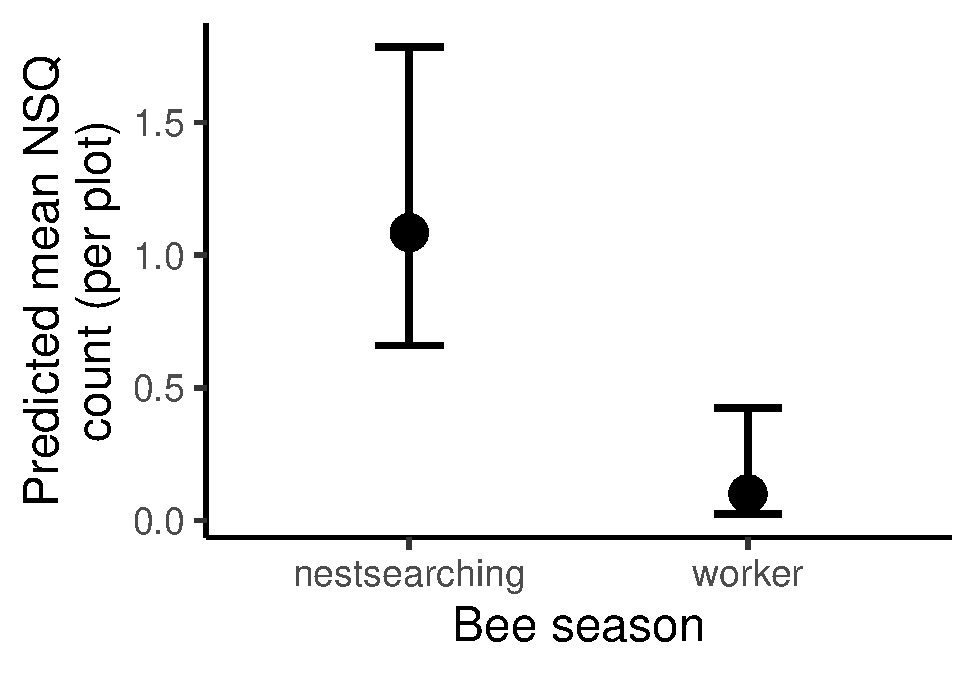
\includegraphics[keepaspectratio]{ch1_glm_clean_files/figure-latex/unnamed-chunk-32-1.pdf}}

\subsection{Findings}\label{findings-3}

In conditional model (modelling abundance of nest-searching queens):

\begin{itemize}
\item
  no significant effect of grass+forb\%, floral abundance, bee season
\item
  significant positive effect of number of burrows
\end{itemize}

In zero-inflation model (modelling presence/absence of nest-searching
queens):

\begin{itemize}
\item
  no significant effect of floral abundance
\item
  Significant effect of grass+forb\% (less likely to be absent with more
  grass/forb), number of burrows (more likely to be absent with more
  burrows), bee season (more likely to be absent during worker season
  than nest-searching season).
\end{itemize}

Interestingly, the number of rodent burrows is associated with more
bombus nest-searching in the conditional model, but the number of rodent
burrows is associated with more structural zeros in the zero-inflation
model. This means that if a site is suitable for nesting, more rodent
burrows is associated with more bombus nest-searching. However, in some
cases, rodent burrows may signal inhospitable habitat conditions for
bumble bees.

\section{Number of workers vs nest-searching queens, floral abundance,
rodent
burrows.}\label{number-of-workers-vs-nest-searching-queens-floral-abundance-rodent-burrows.}

Go through similar model selection steps as for the rodent burrow model.

\subsection{Steps}\label{steps-4}

\begin{enumerate}
\def\labelenumi{\arabic{enumi})}
\tightlist
\item
  Check different random effects structures
\end{enumerate}

\begin{itemize}
\tightlist
\item
  best fit = 1\textbar site\_id/plot\_id --\textgreater{} \textbf{area
  not included}
\end{itemize}

\begin{Shaded}
\begin{Highlighting}[]
\NormalTok{workers\_full }\OtherTok{\textless{}{-}} \FunctionTok{glmmTMB}\NormalTok{(workers }\SpecialCharTok{\textasciitilde{}}\NormalTok{ nest\_searching\_queens\_scaled }\SpecialCharTok{+}
\NormalTok{                       bombus\_floral\_abun\_scaled }\SpecialCharTok{+} 
\NormalTok{                       num\_burrows\_scaled }\SpecialCharTok{+} 
\NormalTok{                         prop\_inactive\_scaled }\SpecialCharTok{+}
\NormalTok{                       bee\_season\_type }\SpecialCharTok{+}
\NormalTok{                         (}\DecValTok{1}\SpecialCharTok{|}\NormalTok{area}\SpecialCharTok{/}\NormalTok{site\_id}\SpecialCharTok{/}\NormalTok{plot\_id), }
                     \AttributeTok{family =}\NormalTok{ poisson,}
                     \AttributeTok{data =}\NormalTok{ field\_data}
\NormalTok{                       )}


\NormalTok{workers\_noArea }\OtherTok{\textless{}{-}} \FunctionTok{glmmTMB}\NormalTok{(workers }\SpecialCharTok{\textasciitilde{}}\NormalTok{ nest\_searching\_queens\_scaled }\SpecialCharTok{+}
\NormalTok{                       bombus\_floral\_abun\_scaled }\SpecialCharTok{+} 
\NormalTok{                       num\_burrows\_scaled }\SpecialCharTok{+} 
\NormalTok{                         prop\_inactive\_scaled }\SpecialCharTok{+}
\NormalTok{                       bee\_season\_type}\SpecialCharTok{+}
\NormalTok{                         (}\DecValTok{1}\SpecialCharTok{|}\NormalTok{site\_id}\SpecialCharTok{/}\NormalTok{plot\_id), }
                     \AttributeTok{family =}\NormalTok{ poisson,}
                     \AttributeTok{data =}\NormalTok{ field\_data}
\NormalTok{                       )}

\NormalTok{workers\_plotOnly }\OtherTok{\textless{}{-}}  \FunctionTok{glmmTMB}\NormalTok{(workers }\SpecialCharTok{\textasciitilde{}}\NormalTok{ nest\_searching\_queens\_scaled }\SpecialCharTok{+}
\NormalTok{                       bombus\_floral\_abun\_scaled }\SpecialCharTok{+} 
\NormalTok{                       num\_burrows\_scaled }\SpecialCharTok{+} 
\NormalTok{                         prop\_inactive\_scaled }\SpecialCharTok{+}
\NormalTok{                       bee\_season\_type}\SpecialCharTok{+}
\NormalTok{                         (}\DecValTok{1}\SpecialCharTok{|}\NormalTok{plot\_id), }
                     \AttributeTok{family =}\NormalTok{ poisson,}
                     \AttributeTok{data =}\NormalTok{ field\_data}
\NormalTok{                       )}

\NormalTok{workers\_siteOnly }\OtherTok{\textless{}{-}} \FunctionTok{glmmTMB}\NormalTok{(workers }\SpecialCharTok{\textasciitilde{}}\NormalTok{ nest\_searching\_queens\_scaled }\SpecialCharTok{+}
\NormalTok{                       bombus\_floral\_abun\_scaled }\SpecialCharTok{+} 
\NormalTok{                       num\_burrows\_scaled }\SpecialCharTok{+} 
\NormalTok{                         prop\_inactive\_scaled }\SpecialCharTok{+}
\NormalTok{                       bee\_season\_type}\SpecialCharTok{+}
\NormalTok{                         (}\DecValTok{1}\SpecialCharTok{|}\NormalTok{site\_id), }
                     \AttributeTok{family =}\NormalTok{ poisson,}
                     \AttributeTok{data =}\NormalTok{ field\_data}
\NormalTok{                       )}

\NormalTok{workers\_AreaPlot }\OtherTok{\textless{}{-}}  \FunctionTok{glmmTMB}\NormalTok{(workers }\SpecialCharTok{\textasciitilde{}}\NormalTok{ nest\_searching\_queens\_scaled }\SpecialCharTok{+}
\NormalTok{                       bombus\_floral\_abun\_scaled }\SpecialCharTok{+} 
\NormalTok{                       num\_burrows\_scaled }\SpecialCharTok{+} 
\NormalTok{                         prop\_inactive\_scaled }\SpecialCharTok{+}
\NormalTok{                       bee\_season\_type}\SpecialCharTok{+}
\NormalTok{                         (}\DecValTok{1}\SpecialCharTok{|}\NormalTok{area}\SpecialCharTok{/}\NormalTok{plot\_id), }
                     \AttributeTok{family =}\NormalTok{ poisson,}
                     \AttributeTok{data =}\NormalTok{ field\_data}
\NormalTok{                       )}

\NormalTok{workers\_noRE }\OtherTok{\textless{}{-}} \FunctionTok{glmmTMB}\NormalTok{(workers }\SpecialCharTok{\textasciitilde{}}\NormalTok{ nest\_searching\_queens\_scaled }\SpecialCharTok{+}
\NormalTok{                       bombus\_floral\_abun\_scaled }\SpecialCharTok{+} 
\NormalTok{                       num\_burrows\_scaled }\SpecialCharTok{+} 
\NormalTok{                         prop\_inactive\_scaled }\SpecialCharTok{+}
\NormalTok{                       bee\_season\_type, }
                     \AttributeTok{family =}\NormalTok{ poisson,}
                     \AttributeTok{data =}\NormalTok{ field\_data}
\NormalTok{                       )}

\CommentTok{\#compare models using maximum likelihood test}
\FunctionTok{anova}\NormalTok{(workers\_full, workers\_noArea, workers\_plotOnly, workers\_siteOnly, workers\_AreaPlot, workers\_noRE)}
\end{Highlighting}
\end{Shaded}

\begin{verbatim}
## Data: field_data
## Models:
## workers_noRE: workers ~ nest_searching_queens_scaled + bombus_floral_abun_scaled + , zi=~0, disp=~1
## workers_noRE:     num_burrows_scaled + prop_inactive_scaled + bee_season_type, zi=~0, disp=~1
## workers_plotOnly: workers ~ nest_searching_queens_scaled + bombus_floral_abun_scaled + , zi=~0, disp=~1
## workers_plotOnly:     num_burrows_scaled + prop_inactive_scaled + bee_season_type + , zi=~0, disp=~1
## workers_plotOnly:     (1 | plot_id), zi=~0, disp=~1
## workers_siteOnly: workers ~ nest_searching_queens_scaled + bombus_floral_abun_scaled + , zi=~0, disp=~1
## workers_siteOnly:     num_burrows_scaled + prop_inactive_scaled + bee_season_type + , zi=~0, disp=~1
## workers_siteOnly:     (1 | site_id), zi=~0, disp=~1
## workers_noArea: workers ~ nest_searching_queens_scaled + bombus_floral_abun_scaled + , zi=~0, disp=~1
## workers_noArea:     num_burrows_scaled + prop_inactive_scaled + bee_season_type + , zi=~0, disp=~1
## workers_noArea:     (1 | site_id/plot_id), zi=~0, disp=~1
## workers_AreaPlot: workers ~ nest_searching_queens_scaled + bombus_floral_abun_scaled + , zi=~0, disp=~1
## workers_AreaPlot:     num_burrows_scaled + prop_inactive_scaled + bee_season_type + , zi=~0, disp=~1
## workers_AreaPlot:     (1 | area/plot_id), zi=~0, disp=~1
## workers_full: workers ~ nest_searching_queens_scaled + bombus_floral_abun_scaled + , zi=~0, disp=~1
## workers_full:     num_burrows_scaled + prop_inactive_scaled + bee_season_type + , zi=~0, disp=~1
## workers_full:     (1 | area/site_id/plot_id), zi=~0, disp=~1
##                  Df    AIC    BIC  logLik deviance  Chisq Chi Df Pr(>Chisq)    
## workers_noRE      6 175.50 192.02 -81.748   163.50                             
## workers_plotOnly  7 173.90 193.18 -79.952   159.90 3.5910      1    0.05809 .  
## workers_siteOnly  7 165.67 184.95 -75.836   151.67 8.2316      0    < 2e-16 ***
## workers_noArea    8 164.91 186.94 -74.455   148.91 2.7629      1    0.09647 .  
## workers_AreaPlot  8 168.75 190.78 -76.374   152.75 0.0000      0    1.00000    
## workers_full      9 166.91 191.69 -74.455   148.91 3.8374      1    0.05012 .  
## ---
## Signif. codes:  0 '***' 0.001 '**' 0.01 '*' 0.05 '.' 0.1 ' ' 1
\end{verbatim}

\begin{Shaded}
\begin{Highlighting}[]
\DocumentationTok{\#\#results tells us the model with no area is best (lowest AIC). }
\end{Highlighting}
\end{Shaded}

\begin{enumerate}
\def\labelenumi{\arabic{enumi}.}
\setcounter{enumi}{1}
\tightlist
\item
  Check diagnostics of best model.
\end{enumerate}

\begin{itemize}
\tightlist
\item
  No significant diagnostic tests. Good to go.
\end{itemize}

\begin{Shaded}
\begin{Highlighting}[]
\CommentTok{\#simulate residuals}
\NormalTok{residuals\_workers\_noArea }\OtherTok{\textless{}{-}} \FunctionTok{simulateResiduals}\NormalTok{(}\AttributeTok{fittedModel =}\NormalTok{ workers\_noArea, }\AttributeTok{plot =} \ConstantTok{TRUE}\NormalTok{)}
\end{Highlighting}
\end{Shaded}

\pandocbounded{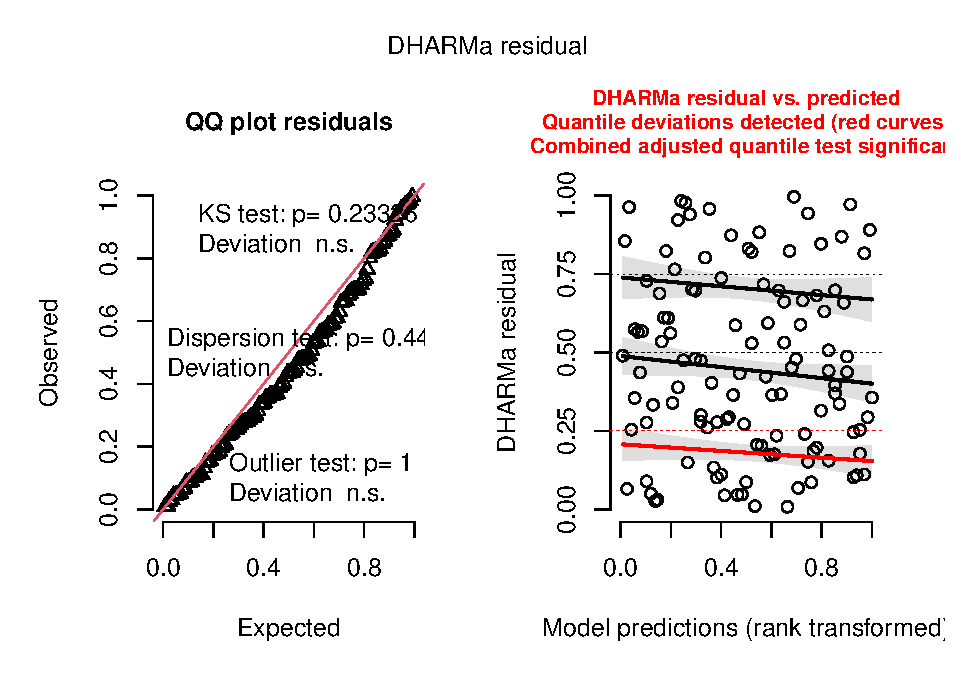
\includegraphics[keepaspectratio]{ch1_glm_clean_files/figure-latex/unnamed-chunk-34-1.pdf}}

\begin{enumerate}
\def\labelenumi{\arabic{enumi}.}
\setcounter{enumi}{2}
\tightlist
\item
  Check results of final model
\end{enumerate}

\begin{Shaded}
\begin{Highlighting}[]
\FunctionTok{summary}\NormalTok{(workers\_noArea)}
\end{Highlighting}
\end{Shaded}

\begin{verbatim}
##  Family: poisson  ( log )
## Formula:          
## workers ~ nest_searching_queens_scaled + bombus_floral_abun_scaled +  
##     num_burrows_scaled + prop_inactive_scaled + bee_season_type +  
##     (1 | site_id/plot_id)
## Data: field_data
## 
##       AIC       BIC    logLik -2*log(L)  df.resid 
##     164.9     186.9     -74.5     148.9       108 
## 
## Random effects:
## 
## Conditional model:
##  Groups          Name        Variance Std.Dev.
##  plot_id:site_id (Intercept) 0.7704   0.8777  
##  site_id         (Intercept) 0.2976   0.5455  
## Number of obs: 116, groups:  plot_id:site_id, 20; site_id, 11
## 
## Conditional model:
##                              Estimate Std. Error z value Pr(>|z|)    
## (Intercept)                  -3.56408    0.65332  -5.455 4.89e-08 ***
## nest_searching_queens_scaled  0.01148    0.55155   0.021 0.983388    
## bombus_floral_abun_scaled     0.71632    0.22172   3.231 0.001235 ** 
## num_burrows_scaled            0.31621    0.37307   0.848 0.396675    
## prop_inactive_scaled         -0.18788    0.35360  -0.531 0.595182    
## bee_season_typeworker         2.33515    0.61408   3.803 0.000143 ***
## ---
## Signif. codes:  0 '***' 0.001 '**' 0.01 '*' 0.05 '.' 0.1 ' ' 1
\end{verbatim}

\subsection{Plots}\label{plots-4}

Number of workers vs number of nest-searching queens

\begin{Shaded}
\begin{Highlighting}[]
\CommentTok{\# Define a sequence of values for nsq across its observed range}
\NormalTok{queen\_seq }\OtherTok{\textless{}{-}} \FunctionTok{seq}\NormalTok{(}
  \AttributeTok{from =} \FunctionTok{min}\NormalTok{(field\_data}\SpecialCharTok{$}\NormalTok{nest\_searching\_queens\_scaled, }\AttributeTok{na.rm =} \ConstantTok{TRUE}\NormalTok{),}
  \AttributeTok{to =} \FunctionTok{max}\NormalTok{(field\_data}\SpecialCharTok{$}\NormalTok{nest\_searching\_queens\_scaled, }\AttributeTok{na.rm =} \ConstantTok{TRUE}\NormalTok{),}
  \AttributeTok{length.out =} \DecValTok{50}
\NormalTok{)}

\CommentTok{\#create new data grid}
\NormalTok{worker\_data\_nsq}\OtherTok{\textless{}{-}} \FunctionTok{expand.grid}\NormalTok{(}
  \AttributeTok{nest\_searching\_queens\_scaled =}\NormalTok{ queen\_seq,}
  \AttributeTok{bombus\_floral\_abun\_scaled =} \FunctionTok{mean}\NormalTok{(field\_data}\SpecialCharTok{$}\NormalTok{bombus\_floral\_abun\_scaled, }\AttributeTok{na.rm =} \ConstantTok{TRUE}\NormalTok{),}
  \AttributeTok{num\_burrows\_scaled =} \FunctionTok{mean}\NormalTok{(field\_data}\SpecialCharTok{$}\NormalTok{num\_burrows\_scaled, }\AttributeTok{na.rm =} \ConstantTok{TRUE}\NormalTok{),}
  \AttributeTok{prop\_inactive\_scaled =} \FunctionTok{mean}\NormalTok{(field\_data}\SpecialCharTok{$}\NormalTok{prop\_inactive\_scaled, }\AttributeTok{na.rm =} \ConstantTok{TRUE}\NormalTok{),}
  \AttributeTok{bee\_season\_type =} \StringTok{"worker"}
\NormalTok{)}

\CommentTok{\# Get predicted probabilities and standard errors}
\NormalTok{pred\_worker\_nsq }\OtherTok{\textless{}{-}} \FunctionTok{predict}\NormalTok{(workers\_noArea,}
                            \AttributeTok{newdata =}\NormalTok{ worker\_data\_nsq,}
                           \AttributeTok{type =} \StringTok{"link"}\NormalTok{,}
                            \AttributeTok{se.fit =} \ConstantTok{TRUE}\NormalTok{,}
                            \AttributeTok{re.form =} \ConstantTok{NA}\NormalTok{)}

\CommentTok{\# Combine predictions with data frame}
\NormalTok{pred\_worker\_nsq\_df }\OtherTok{\textless{}{-}} \FunctionTok{cbind}\NormalTok{(worker\_data\_nsq,}
                 \AttributeTok{fit\_log =}\NormalTok{ pred\_worker\_nsq}\SpecialCharTok{$}\NormalTok{fit,}
                 \AttributeTok{se\_log =}\NormalTok{ pred\_worker\_nsq}\SpecialCharTok{$}\NormalTok{se.fit)}

\CommentTok{\#calculate predictions and confidence intervals on response scale (not log scale)}
\NormalTok{pred\_worker\_nsq\_df }\OtherTok{\textless{}{-}}\NormalTok{ pred\_worker\_nsq\_df }\SpecialCharTok{\%\textgreater{}\%}
  \FunctionTok{mutate}\NormalTok{(}
    \AttributeTok{fit =} \FunctionTok{exp}\NormalTok{(fit\_log),}
    \AttributeTok{lower =} \FunctionTok{exp}\NormalTok{(fit\_log }\SpecialCharTok{{-}} \FloatTok{1.96} \SpecialCharTok{*}\NormalTok{ se\_log),}
    \AttributeTok{upper =} \FunctionTok{exp}\NormalTok{(fit\_log }\SpecialCharTok{+} \FloatTok{1.96} \SpecialCharTok{*}\NormalTok{ se\_log)}
\NormalTok{  )}

\FunctionTok{ggplot}\NormalTok{(pred\_worker\_nsq\_df, }\FunctionTok{aes}\NormalTok{(}\AttributeTok{x =}\NormalTok{ nest\_searching\_queens\_scaled, }\AttributeTok{y =}\NormalTok{ fit)) }\SpecialCharTok{+}
  \FunctionTok{geom\_line}\NormalTok{(}\AttributeTok{size =} \DecValTok{3}\NormalTok{) }\SpecialCharTok{+}
  \FunctionTok{geom\_ribbon}\NormalTok{(}\FunctionTok{aes}\NormalTok{(}\AttributeTok{ymin =}\NormalTok{ lower, }\AttributeTok{ymax =}\NormalTok{ upper), }\AttributeTok{alpha =} \FloatTok{0.2}\NormalTok{) }\SpecialCharTok{+}
  \FunctionTok{labs}\NormalTok{(}
       \AttributeTok{x =} \StringTok{"NSQ abundance (scaled)"}\NormalTok{,}
       \AttributeTok{y =} \StringTok{"Predicted mean worker}\SpecialCharTok{\textbackslash{}n}\StringTok{count (per plot)"}\NormalTok{) }\SpecialCharTok{+}
  \FunctionTok{theme\_classic}\NormalTok{(}\AttributeTok{base\_size =} \DecValTok{23}\NormalTok{)}
\end{Highlighting}
\end{Shaded}

\pandocbounded{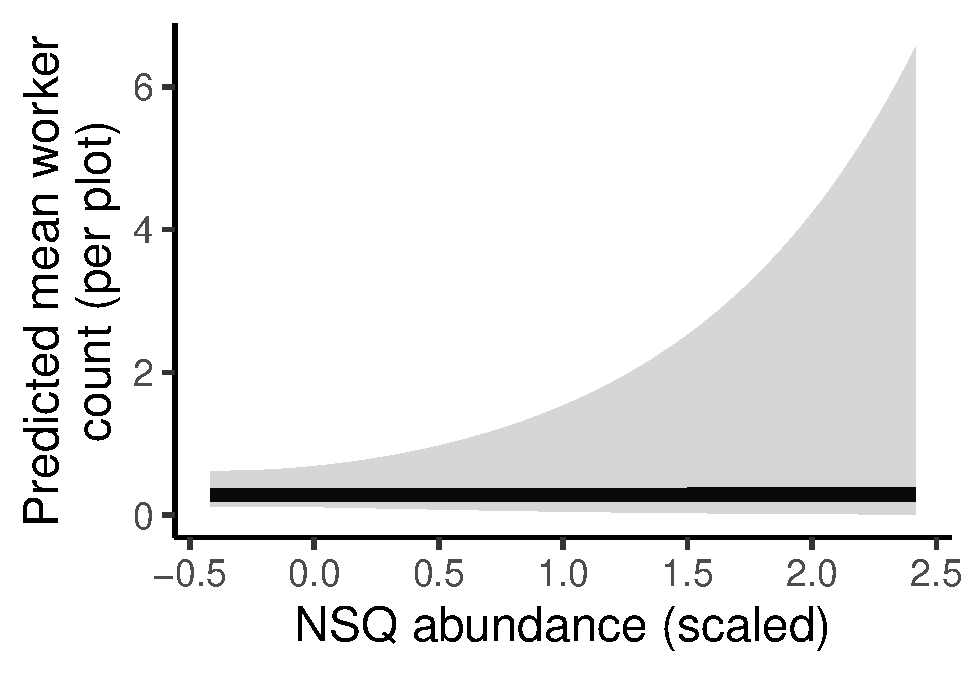
\includegraphics[keepaspectratio]{ch1_glm_clean_files/figure-latex/unnamed-chunk-36-1.pdf}}

Number of workers vs floral abundance

\begin{Shaded}
\begin{Highlighting}[]
\CommentTok{\#create new data grid}
\NormalTok{worker\_data\_floral}\OtherTok{\textless{}{-}} \FunctionTok{expand.grid}\NormalTok{(}
  \AttributeTok{nest\_searching\_queens\_scaled =} \FunctionTok{mean}\NormalTok{(field\_data}\SpecialCharTok{$}\NormalTok{nest\_searching\_queens\_scaled, }\AttributeTok{na.rm =} \ConstantTok{TRUE}\NormalTok{),}
  \AttributeTok{bombus\_floral\_abun\_scaled =}\NormalTok{ floral\_seq,}
  \AttributeTok{num\_burrows\_scaled =} \FunctionTok{mean}\NormalTok{(field\_data}\SpecialCharTok{$}\NormalTok{num\_burrows\_scaled, }\AttributeTok{na.rm =} \ConstantTok{TRUE}\NormalTok{),}
  \AttributeTok{prop\_inactive\_scaled =} \FunctionTok{mean}\NormalTok{(field\_data}\SpecialCharTok{$}\NormalTok{prop\_inactive\_scaled, }\AttributeTok{na.rm =} \ConstantTok{TRUE}\NormalTok{),}
  \AttributeTok{bee\_season\_type =} \StringTok{"worker"}
\NormalTok{)}

\CommentTok{\# Get predicted probabilities and standard errors}
\NormalTok{pred\_worker\_floral }\OtherTok{\textless{}{-}} \FunctionTok{predict}\NormalTok{(workers\_noArea,}
                            \AttributeTok{newdata =}\NormalTok{ worker\_data\_floral,}
                            \AttributeTok{type =} \StringTok{"link"}\NormalTok{,}
                            \AttributeTok{se.fit =} \ConstantTok{TRUE}\NormalTok{,}
                            \AttributeTok{re.form =} \ConstantTok{NA}\NormalTok{)}

\CommentTok{\# Combine predictions with data frame}
\NormalTok{pred\_worker\_floral\_df }\OtherTok{\textless{}{-}} \FunctionTok{cbind}\NormalTok{(worker\_data\_floral,}
                 \AttributeTok{fit\_log =}\NormalTok{ pred\_worker\_floral}\SpecialCharTok{$}\NormalTok{fit,}
                 \AttributeTok{se\_log =}\NormalTok{ pred\_worker\_floral}\SpecialCharTok{$}\NormalTok{se.fit)}

\CommentTok{\#calculate predictions and confidence intervals on response scale (not log scale)}
\NormalTok{pred\_worker\_floral\_df }\OtherTok{\textless{}{-}}\NormalTok{ pred\_worker\_floral\_df }\SpecialCharTok{\%\textgreater{}\%}
  \FunctionTok{mutate}\NormalTok{(}
    \AttributeTok{fit =} \FunctionTok{exp}\NormalTok{(fit\_log),}
    \AttributeTok{lower =} \FunctionTok{exp}\NormalTok{(fit\_log }\SpecialCharTok{{-}} \FloatTok{1.96} \SpecialCharTok{*}\NormalTok{ se\_log),}
    \AttributeTok{upper =} \FunctionTok{exp}\NormalTok{(fit\_log }\SpecialCharTok{+} \FloatTok{1.96} \SpecialCharTok{*}\NormalTok{ se\_log)}
\NormalTok{  )}

\FunctionTok{ggplot}\NormalTok{(pred\_worker\_floral\_df, }\FunctionTok{aes}\NormalTok{(}\AttributeTok{x =}\NormalTok{ bombus\_floral\_abun\_scaled, }\AttributeTok{y =}\NormalTok{ fit)) }\SpecialCharTok{+}
  \FunctionTok{geom\_line}\NormalTok{(}\AttributeTok{size =} \DecValTok{3}\NormalTok{) }\SpecialCharTok{+}
  \FunctionTok{geom\_ribbon}\NormalTok{(}\FunctionTok{aes}\NormalTok{(}\AttributeTok{ymin =}\NormalTok{ lower, }\AttributeTok{ymax =}\NormalTok{ upper), }\AttributeTok{alpha =} \FloatTok{0.2}\NormalTok{) }\SpecialCharTok{+}
  \FunctionTok{labs}\NormalTok{(}
       \AttributeTok{x =} \StringTok{"Floral abundance (scaled)"}\NormalTok{,}
       \AttributeTok{y =} \StringTok{"Predicted mean worker}\SpecialCharTok{\textbackslash{}n}\StringTok{count (per plot)"}\NormalTok{) }\SpecialCharTok{+}
  \FunctionTok{theme\_classic}\NormalTok{(}\AttributeTok{base\_size =} \DecValTok{23}\NormalTok{)}
\end{Highlighting}
\end{Shaded}

\pandocbounded{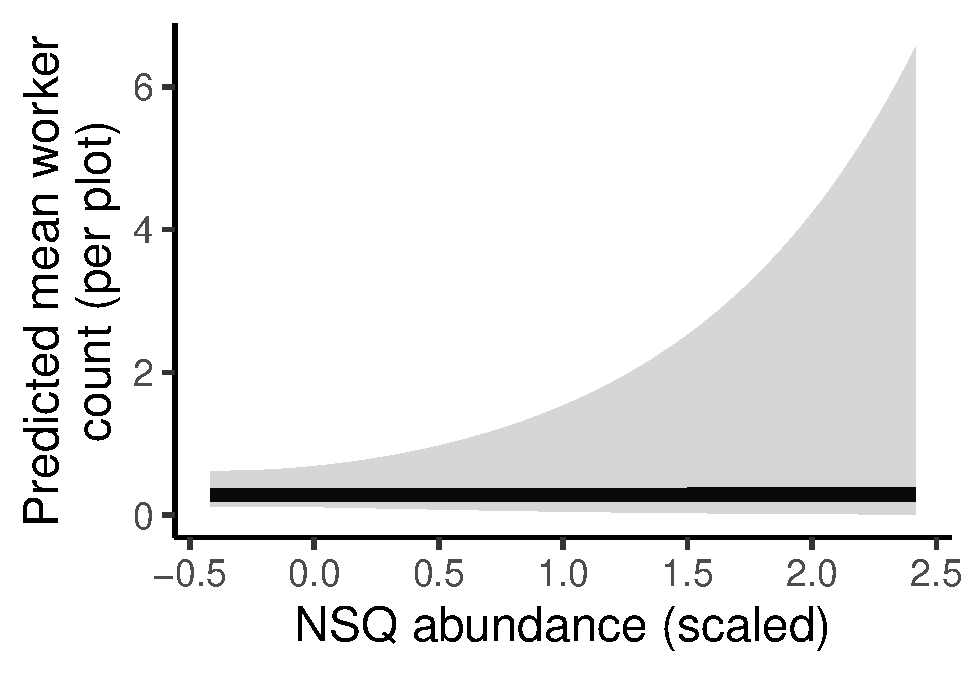
\includegraphics[keepaspectratio]{ch1_glm_clean_files/figure-latex/unnamed-chunk-37-1.pdf}}

Number of workers vs number of rodent burrows

\begin{Shaded}
\begin{Highlighting}[]
\CommentTok{\# Define a sequence of values for rodent burrows across its observed range}
\NormalTok{rodent\_seq }\OtherTok{\textless{}{-}} \FunctionTok{seq}\NormalTok{(}
  \AttributeTok{from =} \FunctionTok{min}\NormalTok{(field\_data}\SpecialCharTok{$}\NormalTok{num\_burrows\_scaled, }\AttributeTok{na.rm =} \ConstantTok{TRUE}\NormalTok{),}
  \AttributeTok{to =} \FunctionTok{max}\NormalTok{(field\_data}\SpecialCharTok{$}\NormalTok{num\_burrows\_scaled, }\AttributeTok{na.rm =} \ConstantTok{TRUE}\NormalTok{),}
  \AttributeTok{length.out =} \DecValTok{50}\NormalTok{)}

\CommentTok{\#create new data grid}
\NormalTok{worker\_data\_rodent}\OtherTok{\textless{}{-}} \FunctionTok{expand.grid}\NormalTok{(}
  \AttributeTok{nest\_searching\_queens\_scaled =} \FunctionTok{mean}\NormalTok{(field\_data}\SpecialCharTok{$}\NormalTok{nest\_searching\_queens\_scaled, }\AttributeTok{na.rm =} \ConstantTok{TRUE}\NormalTok{),}
  \AttributeTok{bombus\_floral\_abun\_scaled =} \FunctionTok{mean}\NormalTok{(field\_data}\SpecialCharTok{$}\NormalTok{bombus\_floral\_abun\_scaled, }\AttributeTok{na.rm =} \ConstantTok{TRUE}\NormalTok{),}
  \AttributeTok{num\_burrows\_scaled =}\NormalTok{rodent\_seq,}
  \AttributeTok{prop\_inactive\_scaled =} \FunctionTok{mean}\NormalTok{(field\_data}\SpecialCharTok{$}\NormalTok{prop\_inactive\_scaled, }\AttributeTok{na.rm =} \ConstantTok{TRUE}\NormalTok{),}
  \AttributeTok{bee\_season\_type =} \StringTok{"worker"}
\NormalTok{)}

\CommentTok{\# Get predicted probabilities and standard errors}
\NormalTok{pred\_worker\_rodent }\OtherTok{\textless{}{-}} \FunctionTok{predict}\NormalTok{(workers\_noArea,}
                            \AttributeTok{newdata =}\NormalTok{ worker\_data\_rodent,}
                            \AttributeTok{type =} \StringTok{"link"}\NormalTok{,}
                            \AttributeTok{se.fit =} \ConstantTok{TRUE}\NormalTok{,}
                            \AttributeTok{re.form =} \ConstantTok{NA}\NormalTok{)}

\CommentTok{\# Combine predictions with data frame}
\NormalTok{pred\_worker\_rodent\_df }\OtherTok{\textless{}{-}} \FunctionTok{cbind}\NormalTok{(worker\_data\_rodent,}
                 \AttributeTok{fit\_log =}\NormalTok{ pred\_worker\_rodent}\SpecialCharTok{$}\NormalTok{fit,}
                 \AttributeTok{se\_log =}\NormalTok{ pred\_worker\_rodent}\SpecialCharTok{$}\NormalTok{se.fit)}

\CommentTok{\#calculate predictions and confidence intervals on response scale (not log scale)}
\NormalTok{pred\_worker\_rodent\_df }\OtherTok{\textless{}{-}}\NormalTok{ pred\_worker\_rodent\_df }\SpecialCharTok{\%\textgreater{}\%}
  \FunctionTok{mutate}\NormalTok{(}
    \AttributeTok{fit =} \FunctionTok{exp}\NormalTok{(fit\_log),}
    \AttributeTok{lower =} \FunctionTok{exp}\NormalTok{(fit\_log }\SpecialCharTok{{-}} \FloatTok{1.96} \SpecialCharTok{*}\NormalTok{ se\_log),}
    \AttributeTok{upper =} \FunctionTok{exp}\NormalTok{(fit\_log }\SpecialCharTok{+} \FloatTok{1.96} \SpecialCharTok{*}\NormalTok{ se\_log)}
\NormalTok{  )}

\FunctionTok{ggplot}\NormalTok{(pred\_worker\_rodent\_df, }\FunctionTok{aes}\NormalTok{(}\AttributeTok{x =}\NormalTok{ num\_burrows\_scaled, }\AttributeTok{y =}\NormalTok{ fit)) }\SpecialCharTok{+}
  \FunctionTok{geom\_line}\NormalTok{(}\AttributeTok{size =} \DecValTok{3}\NormalTok{) }\SpecialCharTok{+}
  \FunctionTok{geom\_ribbon}\NormalTok{(}\FunctionTok{aes}\NormalTok{(}\AttributeTok{ymin =}\NormalTok{ lower, }\AttributeTok{ymax =}\NormalTok{ upper), }\AttributeTok{alpha =} \FloatTok{0.2}\NormalTok{) }\SpecialCharTok{+}
  \FunctionTok{labs}\NormalTok{(}
       \AttributeTok{x =} \StringTok{"Burrow abundance (scaled)"}\NormalTok{,}
       \AttributeTok{y =} \StringTok{"Predicted mean worker}\SpecialCharTok{\textbackslash{}n}\StringTok{count (per plot)"}\NormalTok{) }\SpecialCharTok{+}
  \FunctionTok{theme\_classic}\NormalTok{(}\AttributeTok{base\_size =} \DecValTok{23}\NormalTok{)}
\end{Highlighting}
\end{Shaded}

\pandocbounded{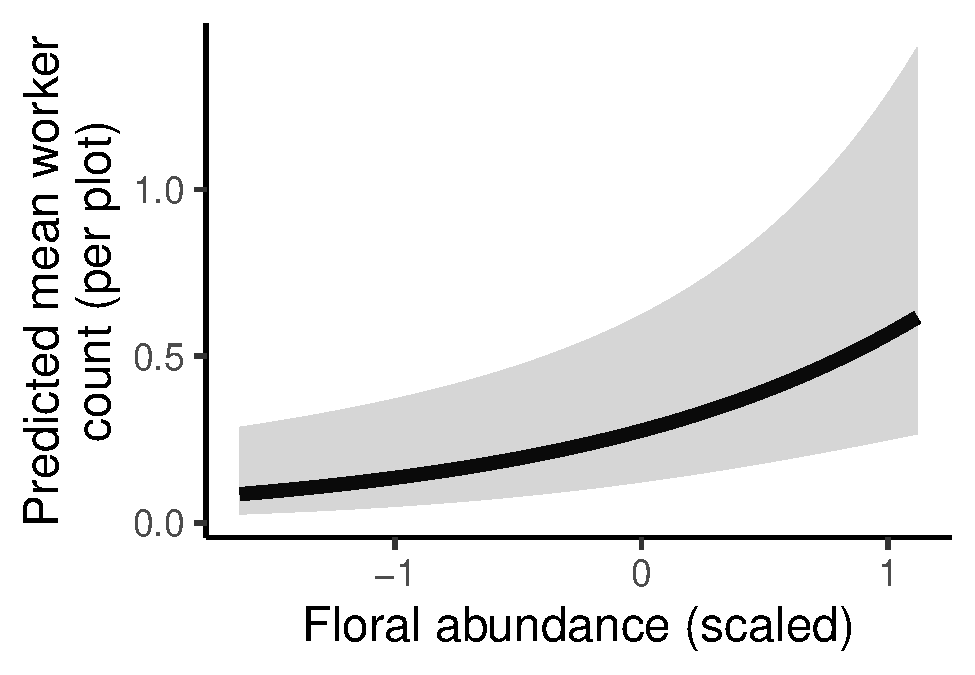
\includegraphics[keepaspectratio]{ch1_glm_clean_files/figure-latex/unnamed-chunk-38-1.pdf}}

Number of workers vs burrow vacancy proportion

\begin{Shaded}
\begin{Highlighting}[]
\CommentTok{\#create new data grid}
\NormalTok{worker\_data\_vacancy }\OtherTok{\textless{}{-}} \FunctionTok{expand.grid}\NormalTok{(}
  \AttributeTok{nest\_searching\_queens\_scaled =} \FunctionTok{mean}\NormalTok{(field\_data}\SpecialCharTok{$}\NormalTok{nest\_searching\_queens\_scaled, }\AttributeTok{na.rm =} \ConstantTok{TRUE}\NormalTok{),}
  \AttributeTok{bombus\_floral\_abun\_scaled =} \FunctionTok{mean}\NormalTok{(field\_data}\SpecialCharTok{$}\NormalTok{bombus\_floral\_abun\_scaled, }\AttributeTok{na.rm =} \ConstantTok{TRUE}\NormalTok{),}
  \AttributeTok{num\_burrows\_scaled =}\FunctionTok{mean}\NormalTok{(field\_data}\SpecialCharTok{$}\NormalTok{num\_burrows\_scaled, }\AttributeTok{na.rm =} \ConstantTok{TRUE}\NormalTok{),}
  \AttributeTok{bee\_season\_type =} \StringTok{"worker"}\NormalTok{,}
  \AttributeTok{prop\_inactive\_scaled =} \FunctionTok{seq}\NormalTok{(}\FunctionTok{min}\NormalTok{(field\_data}\SpecialCharTok{$}\NormalTok{prop\_inactive\_scaled, }\AttributeTok{na.rm =} \ConstantTok{TRUE}\NormalTok{), }
                             \FunctionTok{max}\NormalTok{(field\_data}\SpecialCharTok{$}\NormalTok{prop\_inactive\_scaled, }\AttributeTok{na.rm =} \ConstantTok{TRUE}\NormalTok{), }
                             \AttributeTok{length.out =} \DecValTok{50}\NormalTok{)}
\NormalTok{)}

\CommentTok{\# Predictions }
\NormalTok{pred\_worker\_vacancy }\OtherTok{\textless{}{-}} \FunctionTok{predict}\NormalTok{(workers\_noArea,}
                            \AttributeTok{newdata =}\NormalTok{ worker\_data\_vacancy,}
                            \AttributeTok{type =} \StringTok{"link"}\NormalTok{,}
                            \AttributeTok{se.fit =} \ConstantTok{TRUE}\NormalTok{,}
                            \AttributeTok{re.form =} \ConstantTok{NA}
\NormalTok{                            )}

\CommentTok{\# Combine predictions with data frame}
\NormalTok{pred\_worker\_vacancy\_df }\OtherTok{\textless{}{-}} \FunctionTok{cbind}\NormalTok{(worker\_data\_vacancy,}
                 \AttributeTok{fit\_log =}\NormalTok{ pred\_worker\_vacancy}\SpecialCharTok{$}\NormalTok{fit,}
                 \AttributeTok{se\_log =}\NormalTok{ pred\_worker\_vacancy}\SpecialCharTok{$}\NormalTok{se.fit)}

\CommentTok{\#calculate predictions and confidence intervals on response scale (not log scale)}
\NormalTok{pred\_worker\_vacancy\_df }\OtherTok{\textless{}{-}}\NormalTok{ pred\_worker\_vacancy\_df }\SpecialCharTok{\%\textgreater{}\%}
  \FunctionTok{mutate}\NormalTok{(}
    \AttributeTok{fit =} \FunctionTok{exp}\NormalTok{(fit\_log),}
    \AttributeTok{lower =} \FunctionTok{exp}\NormalTok{(fit\_log }\SpecialCharTok{{-}} \FloatTok{1.96} \SpecialCharTok{*}\NormalTok{ se\_log),}
    \AttributeTok{upper =} \FunctionTok{exp}\NormalTok{(fit\_log }\SpecialCharTok{+} \FloatTok{1.96} \SpecialCharTok{*}\NormalTok{ se\_log)}
\NormalTok{  )}

\CommentTok{\#plot}
\FunctionTok{ggplot}\NormalTok{(pred\_worker\_vacancy\_df, }\FunctionTok{aes}\NormalTok{(}\AttributeTok{x =}\NormalTok{ prop\_inactive\_scaled, }\AttributeTok{y =}\NormalTok{ fit)) }\SpecialCharTok{+}
  \FunctionTok{geom\_line}\NormalTok{(}\AttributeTok{linewidth =} \DecValTok{3}\NormalTok{) }\SpecialCharTok{+}
  \FunctionTok{geom\_ribbon}\NormalTok{(}\FunctionTok{aes}\NormalTok{(}\AttributeTok{ymin =}\NormalTok{ lower, }\AttributeTok{ymax =}\NormalTok{ upper), }\AttributeTok{alpha =} \FloatTok{0.2}\NormalTok{) }\SpecialCharTok{+}
  \FunctionTok{labs}\NormalTok{(}
       \AttributeTok{x =} \StringTok{"Proportion of vacant burrows (scaled)"}\NormalTok{,}
       \AttributeTok{y =} \StringTok{"Predicted mean worker}\SpecialCharTok{\textbackslash{}n}\StringTok{count (per plot)"}\NormalTok{) }\SpecialCharTok{+}
  \FunctionTok{theme\_classic}\NormalTok{(}\AttributeTok{base\_size =} \DecValTok{23}\NormalTok{)}
\end{Highlighting}
\end{Shaded}

\pandocbounded{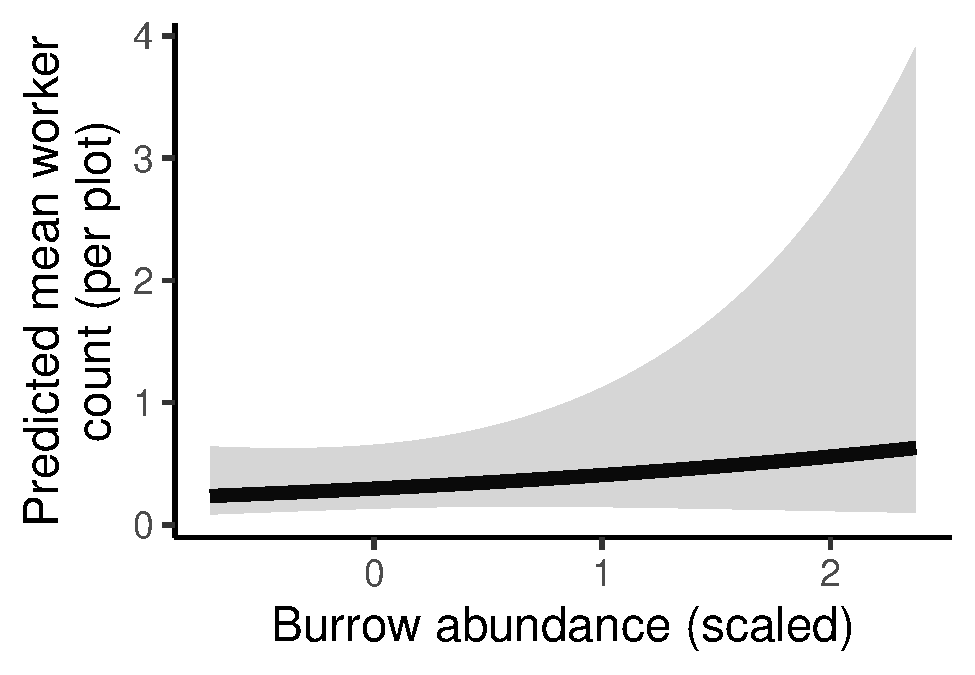
\includegraphics[keepaspectratio]{ch1_glm_clean_files/figure-latex/unnamed-chunk-39-1.pdf}}

Number of workers vs season

\begin{Shaded}
\begin{Highlighting}[]
\CommentTok{\#create new data grid}
\NormalTok{worker\_data\_season}\OtherTok{\textless{}{-}} \FunctionTok{expand.grid}\NormalTok{(}
  \AttributeTok{nest\_searching\_queens\_scaled =} \FunctionTok{mean}\NormalTok{(field\_data}\SpecialCharTok{$}\NormalTok{nest\_searching\_queens\_scaled, }\AttributeTok{na.rm =} \ConstantTok{TRUE}\NormalTok{),}
  \AttributeTok{bombus\_floral\_abun\_scaled =} \FunctionTok{mean}\NormalTok{(field\_data}\SpecialCharTok{$}\NormalTok{bombus\_floral\_abun\_scaled, }\AttributeTok{na.rm =} \ConstantTok{TRUE}\NormalTok{),}
  \AttributeTok{num\_burrows\_scaled =} \FunctionTok{mean}\NormalTok{(field\_data}\SpecialCharTok{$}\NormalTok{num\_burrows\_scaled, }\AttributeTok{na.rm =} \ConstantTok{TRUE}\NormalTok{),}
  \AttributeTok{prop\_inactive\_scaled =} \FunctionTok{mean}\NormalTok{(field\_data}\SpecialCharTok{$}\NormalTok{prop\_inactive\_scaled, }\AttributeTok{na.rm =} \ConstantTok{TRUE}\NormalTok{),}
  \AttributeTok{bee\_season\_type =} \FunctionTok{unique}\NormalTok{(field\_data}\SpecialCharTok{$}\NormalTok{bee\_season\_type)}
\NormalTok{)}

\CommentTok{\# Get predicted probabilities and standard errors}
\NormalTok{pred\_worker\_season }\OtherTok{\textless{}{-}} \FunctionTok{predict}\NormalTok{(workers\_noArea,}
                            \AttributeTok{newdata =}\NormalTok{ worker\_data\_season,}
                            \AttributeTok{type =} \StringTok{"link"}\NormalTok{,}
                            \AttributeTok{se.fit =} \ConstantTok{TRUE}\NormalTok{,}
                            \AttributeTok{re.form =} \ConstantTok{NA}\NormalTok{)}

\CommentTok{\# Combine predictions with data frame}
\NormalTok{pred\_worker\_season\_df }\OtherTok{\textless{}{-}} \FunctionTok{cbind}\NormalTok{(worker\_data\_season,}
                 \AttributeTok{fit\_log =}\NormalTok{ pred\_worker\_season}\SpecialCharTok{$}\NormalTok{fit,}
                 \AttributeTok{se\_log =}\NormalTok{ pred\_worker\_season}\SpecialCharTok{$}\NormalTok{se.fit)}

\CommentTok{\#calculate predictions and confidence intervals on response scale (not log scale)}
\NormalTok{pred\_worker\_season\_df }\OtherTok{\textless{}{-}}\NormalTok{ pred\_worker\_season\_df }\SpecialCharTok{\%\textgreater{}\%}
  \FunctionTok{mutate}\NormalTok{(}
    \AttributeTok{fit =} \FunctionTok{exp}\NormalTok{(fit\_log),}
    \AttributeTok{lower =} \FunctionTok{exp}\NormalTok{(fit\_log }\SpecialCharTok{{-}} \FloatTok{1.96} \SpecialCharTok{*}\NormalTok{ se\_log),}
    \AttributeTok{upper =} \FunctionTok{exp}\NormalTok{(fit\_log }\SpecialCharTok{+} \FloatTok{1.96} \SpecialCharTok{*}\NormalTok{ se\_log)}
\NormalTok{  )}

\FunctionTok{ggplot}\NormalTok{(pred\_worker\_season\_df, }\FunctionTok{aes}\NormalTok{(}\AttributeTok{x =}\NormalTok{ bee\_season\_type, }\AttributeTok{y =}\NormalTok{ fit)) }\SpecialCharTok{+}
  \FunctionTok{geom\_point}\NormalTok{(}\AttributeTok{size =} \DecValTok{8}\NormalTok{) }\SpecialCharTok{+}
  \FunctionTok{geom\_errorbar}\NormalTok{(}\FunctionTok{aes}\NormalTok{(}\AttributeTok{ymin =}\NormalTok{ lower, }\AttributeTok{ymax =}\NormalTok{ upper), }
                \AttributeTok{width =} \FloatTok{0.2}\NormalTok{, }\AttributeTok{position =} \FunctionTok{position\_dodge}\NormalTok{(}\FloatTok{0.6}\NormalTok{), }\AttributeTok{linewidth =} \FloatTok{1.5}\NormalTok{) }\SpecialCharTok{+}
  \FunctionTok{labs}\NormalTok{(}
       \AttributeTok{x =} \StringTok{"Bee season"}\NormalTok{,}
       \AttributeTok{y =} \StringTok{"Predicted mean worker}\SpecialCharTok{\textbackslash{}n}\StringTok{count (per plot)"}\NormalTok{) }\SpecialCharTok{+}
  \FunctionTok{theme\_classic}\NormalTok{(}\AttributeTok{base\_size =} \DecValTok{23}\NormalTok{)}
\end{Highlighting}
\end{Shaded}

\pandocbounded{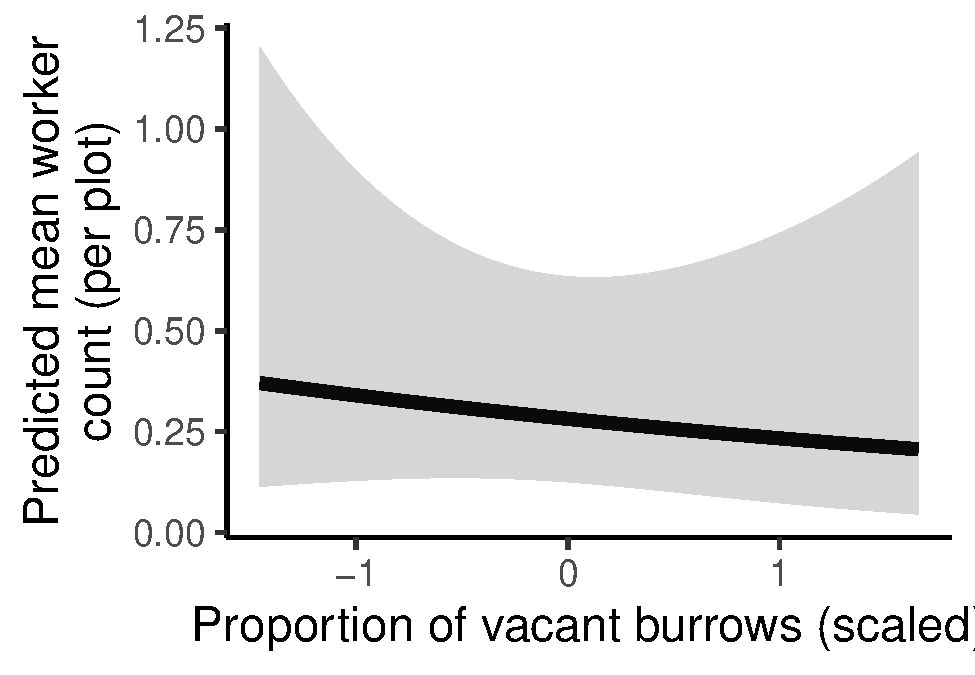
\includegraphics[keepaspectratio]{ch1_glm_clean_files/figure-latex/unnamed-chunk-40-1.pdf}}

\subsection{Findings}\label{findings-4}

Number of nest-searching queens, number of rodent burrows and the
proportion of burrow vacancy does not significantly predict number of
workers. Significantly more workers during worker season than during
nest-searching season. Significant positive effect of bombus-relevant
floral abundance on worker abundance (p=0.0012).

\section{Final Path Diagram}\label{final-path-diagram}

\pandocbounded{
\includegraphics[keepaspectratio]{images/pathDiagramFinal.jpg}}

\end{document}
